\documentclass[../thesis.tex]{subfiles}

\usepackage{wrapfig}
\usepackage{cite}
% \usepackage{natbib}
% \usepackage[round]{natbib}

\usepackage{amsfonts}       % blackboard math symbols
\usepackage{nicefrac}       % compact symbols for 1/2, etc.
\usepackage{microtype}      % microtypography
\usepackage{amsmath}
\usepackage{tikz}
\usepackage{amsthm}
\usepackage{amssymb}
\usetikzlibrary{positioning}
\usepackage{mathtools}

\newtheorem{theorem}{Theorem}[section]
\newtheorem{assumption}{Assumption}[section]
\newtheorem{proposition}{Proposition}[section]
\newtheorem{definition}{Definition}[section]
\newtheorem{corollary}{Corollary}[theorem]
\newtheorem{lemma}{Lemma}[theorem]
% \newtheorem{corollary}{Corollary}[proposition]
\newtheorem{definition1}{Definition}[section]



% %% editing comment
\newcommand{\cmt}[1]{{\footnotesize\textcolor{red}{#1}}}
\newcommand{\cmto}[1]{{\footnotesize\textcolor{orange}{#1}}}
\newcommand{\note}[1]{\cmt{Note: #1}}
\newcommand{\todo}[1]{\cmt{TO-DO: #1}}
\newcommand{\question}[1]{\cmto{Question: #1}}
\newcommand{\sergey}[1]{{\footnotesize\textcolor{blue}{Sergey: #1}}}
\newcommand{\ak}[1]{{\textcolor{red}{#1}}}
\newcommand{\edits}[1]{\textcolor{red}{#1}}

%% abbreviations
\newcommand{\x}{\mathbf{x}}
\newcommand{\z}{\mathbf{z}}
\newcommand{\y}{\mathbf{y}}
\newcommand{\w}{\mathbf{w}}
\newcommand{\data}{\mathcal{D}}

\newcommand{\etal}{{et~al.}\ }
\newcommand{\eg}{e.g.\ }
\newcommand{\ie}{i.e.\ }
\newcommand{\nth}{\text{th}}
\newcommand{\pr}{^\prime}
\newcommand{\tr}{^\mathrm{T}}
\newcommand{\inv}{^{-1}}
\newcommand{\pinv}{^{\dagger}}
\newcommand{\real}{\mathbb{R}}
\newcommand{\gauss}{\mathcal{N}}
\newcommand{\norm}[1]{\left|#1\right|}
\newcommand{\trace}{\text{tr}}

%% specifics for the paper
\newcommand{\reward}{r}
\newcommand{\policy}{\pi}
\newcommand{\mdp}{\mathcal{M}}
\newcommand{\states}{\mathcal{S}}
\newcommand{\actions}{\mathcal{A}}
\newcommand{\observations}{\mathcal{O}}
\newcommand{\transitions}{T}
\newcommand{\initstate}{d_0}
\newcommand{\freq}{d}
\newcommand{\obsfunc}{E}
\newcommand{\initial}{\mathcal{I}}
\newcommand{\horizon}{H}
\newcommand{\rewardevent}{R}
\newcommand{\probr}{p_\rewardevent}
\newcommand{\metareward}{\bar{\reward}}
\newcommand{\discount}{\gamma}
\newcommand{\behavior}{{\pi_\beta}}
\newcommand{\bellman}{\mathcal{B}}
\newcommand{\qparams}{\phi}
\newcommand{\qparamset}{\Phi}
\newcommand{\qset}{\mathcal{Q}}
\newcommand{\batch}{B}
\newcommand{\qfeat}{\mathbf{f}}
\newcommand{\Qfeat}{\mathbf{F}}
\newcommand{\hatbehavior}{\hat{\pi}_\beta}

\newcommand{\traj}{\tau}

\newcommand{\pihi}{\pi^{\text{hi}}}
\newcommand{\pilo}{\pi^{\text{lo}}}
\newcommand{\ah}{\mathbf{w}}

\newcommand{\proj}{\Pi}

\newcommand{\loss}{\mathcal{L}}
\newcommand{\eye}{\mathbf{I}}

\newcommand{\model}{\hat{p}}

\newcommand{\pimix}{\pi_{\text{mix}}}

\newcommand{\pib}{\bar{\pi}}
\newcommand{\epspi}{\epsilon_{\pi}}
\newcommand{\epsmodel}{\epsilon_{m}}

\newcommand{\return}{\mathcal{R}}

%% math
\newcommand{\cY}{\mathcal{Y}}
\newcommand{\cX}{\mathcal{X}}
\newcommand{\en}{\mathcal{E}}
\newcommand{\be}{\mathbf{e}}
\newcommand{\by}{\mathbf{y}}
\newcommand{\bx}{\mathbf{x}}
\newcommand{\bz}{\mathbf{z}}
\newcommand{\bo}{\mathbf{o}}
\newcommand{\bs}{\mathbf{s}}
\newcommand{\ba}{\mathbf{a}}
\newcommand{\bM}{\mathbf{M}}
\newcommand{\ot}{\bo_t}
\newcommand{\st}{\bs_t}
\newcommand{\at}{\ba_t}
\newcommand{\op}{\mathcal{O}}
\newcommand{\opt}{\op_t}
\newcommand{\kl}{D_\text{KL}}
\newcommand{\tv}{D_\text{TV}}
\newcommand{\ent}{\mathcal{H}}

\newcommand{\bzhi}{\bz^\text{hi}}

\newcommand{\E}{\mathbb{E}}

\newenvironment{repeatedthm}[1]{\@begintheorem{#1}{\unskip}}{\@endtheorem}

% \DeclareMathOperator\supp{supp}



\begin{document}


% \blfootnote{This chapter is based on \cite{kumar2020conservative}, published at NeurIPS 2020, which is joint work with Aurick Zhou, George Tucker, and Sergey Levine.}

\vspace{-0.4cm}
\begin{AIbox}{\large{\textbf{Abstract}}}
\vspace{4mm}
In Chapters~\ref{chapter:diagnosing} and \ref{chapter:bear}, we discussed how standard off-policy RL methods can fail in offline RL and how policy constraints can provide for a first approach to tackle distributional shift in offline RL: by simply restricting the support of the learned policy within the support of the behavioral policy, which collected the data. While this approach does lead to promising performance, these methods tend to be restrictive: policy constraints still restrict the learned policy to the behavioral policy even when the Q-function on out-of-distribution actions are not erroneously optimistic to inhibit effective policy learning.                 
% Effectively leveraging large, previously collected datasets in reinforcement learning (RL) is a key challenge for large-scale real-world applications. Offline RL algorithms promise to learn effective policies from previously-collected, static datasets without further interaction. However, in practice, offline RL presents a major challenge, and standard off-policy RL methods can fail due to overestimation of values induced by the distributional shift between the dataset and the learned policy, especially when training on complex and multi-modal data distributions. 
In this chapter, we present a paradigm called \emph{conservative value function estimation}, which aims to address these limitations by learning a value-function such that the expected value of a policy under this value-function lower-bounds its true value. We discuss two concrete variants of this paradigm: a model-free variant, called conservative Q-learning (CQL)~\citep{kumar2020conservative}, and a model-based variant, called conservative offline model-based policy optimization (COMBO)~\citep{yu2021conservative}. Both of these variants can be implemented by augmenting the standard temporal-difference error objective with a Q-value regularizer, on top of model-based and model-free Q-learning and actor-critic algorithms. We will also theoretically show that this paradigm produces conservative value functions, that lower bound the ground-truth value of the current policy, and policies, that enjoy robust policy improvement.
\vspace{2mm}
% CQL produces a lower bound on the value of the current policy and that it can be incorporated into a policy learning procedure with safe improvement guarantees. In practice, CQL augments the standard Bellman error objective with a simple Q-value regularizer which is straightforward to implement on top of standard Q-learning and actor-critic implementations. 
% On both discrete and continuous control domains, we show that CQL substantially outperforms existing offline RL methods, often learning policies that attain 2-5 times higher final return, especially when learning from complex and multi-modal data distributions.
\end{AIbox}

% \blfootnote{Our follow-up on CQL for vision-based robotic manipulation can be found here: \url{https://arxiv.org/abs/2010.14500}.}

\vspace{-0.2cm}
\section{Model-Free Conservative Value Function Estimation}
\label{sec:cql_section}
\vspace{-0.2cm}

\vspace{-0.25cm}
\section{Introduction}
\vspace{-0.25cm}
% motivation: generic RL, and offline RL
Recent advances in reinforcement learning (RL), especially when combined with expressive deep network function approximators, have produced promising results in domains ranging from robotics~\citep{kalashnikov2018qtopt} to strategy games~\citep{alphastar} and recommendation systems~\citep{li2010contextual}. However, applying RL to real-world problems consistently poses practical challenges: in contrast to the kinds of data-driven methods that have been successful in supervised learning~\citep{resnet,bert}, RL is classically regarded as an active learning process, where each training run requires active interaction with the environment. Interaction with the real world can be costly and dangerous, and the quantities of data that can be gathered online are substantially lower than the offline datasets that are used in supervised learning~\citep{imagenet}, which only need to be collected once. Offline RL, also known as batch RL, offers an appealing alternative~\citep{ernst2005tree,fujimoto2018off,kumar2019stabilizing,agarwal2019optimistic,jaques2019way,siegel2020keep,levine2020offline}. Offline RL algorithms learn from large, previously collected datasets, without interaction. This in principle can make it possible to leverage large datasets, but in practice fully offline RL methods pose major technical difficulties, stemming from the distributional shift between the policy that collected the data and the learned policy. This has made current results fall short of the full promise of such methods.

Directly utilizing existing value-based off-policy RL algorithms in an offline setting generally results in poor performance, due to issues with bootstrapping from out-of-distribution actions~\citep{kumar2019stabilizing,fujimoto2018off} and overfitting~\citep{fu2019diagnosing,kumar2019stabilizing,agarwal2019optimistic}. This typically manifests as erroneously optimistic value function estimates.
% motivating the technical approach
If we can instead learn a \emph{conservative} estimate of the value function, which provides a lower bound on the true values, this overestimation problem could be addressed. In fact, because policy evaluation and improvement typically only use the value of the policy, we can learn a less conservative lower bound Q-function, such that only the expected value of Q-function under the policy is lower-bounded, as opposed to a point-wise lower bound.
We propose a novel method for learning such conservative Q-functions via a simple modification to standard value-based RL algorithms. The key idea behind our method is to minimize values under an appropriately chosen distribution over state-action tuples, and then further tighten this bound by also incorporating a \emph{maximization} term over the data distribution.
%%SL.5.2: See the language I used in the abstract to explain this lower bound stuff. I think we could describe the nuance (that we lower bound the expected return of a policy, vs lower bounding the whole Q-function) quite concisely here using similar language.
%% added that

% last para, contributions
Our primary contribution is an algorithmic framework, which we call conservative Q-learning (CQL), for learning conservative, lower-bound estimates of the value function, by regularizing the Q-values during training.
%%SL.5.2: I don't think it's accurate to characterize the method as "simply penalizing" -- but maybe see the language I used in the abstract for inspiration?
Our theoretical analysis of CQL shows that \textit{only} the expected value of this Q-function under the policy lower-bounds the true policy value, preventing extra under-estimation that can arise with point-wise lower-bounded Q-functions, that have typically been explored in the opposite context in exploration literature~\citep{osband2017posterior,jaksch2010near}.
%%SL.5.17: The above sentence is a bit problematic, because I think most readers won't understand its significance. Perhaps we can instead say something like: We present a simplified version of our method that can learn point-wise lower bounds, and then extend this approach to provide a tighter bound that only lower-bounds the expected value under the policy, which also provides improved empirical performance.
%%AK.5.22: I would not prefer calling that a simplified version of our method since that seems like a detail. ALso I wanted to refer more generally to exploration methods that learn point-wise lower bounds, rather than just referring to CQL without the data term. I edited it a bit, but if it does not seem fine to you I can also remove this line.
We also empirically demonstrate the robustness of our approach to Q-function estimation error.
%%SL.5.17: I think we could probably remove this entire sentence.
Our practical algorithm uses these conservative estimates for policy evaluation and offline RL. CQL can be implemented with less than \textbf{20} lines of code on top of a number of standard, online RL algorithms~\citep{haarnoja,dabney2018distributional}, simply by adding the CQL regularization terms to the Q-function update. In our experiments, we demonstrate the efficacy of CQL for offline RL, in domains with complex dataset compositions, where prior methods are typically known to perform poorly~\citep{d4rl} and domains with high-dimensional visual inputs~\citep{bellemare2013arcade,agarwal2019optimistic}. CQL outperforms prior methods by as much as \textbf{2-5x} on many benchmark tasks, and is the only method that can outperform simple behavioral cloning on a number of realistic datasets collected from human interaction.

% \section{Preliminaries}
\label{sec:background}
\vspace{-8pt}
The goal in reinforcement learning is to learn a policy that maximizes the expected cumulative discounted reward in a Markov decision process (MDP), which is defined by a tuple $(\mathcal{S}, \mathcal{A}, \transitions, r, \gamma)$.
$\mathcal{S}, \mathcal{A}$ represent state and action spaces, $\transitions(\bs' | \bs, \mathbf{a})$ and $r(\bs,\mathbf{a})$ represent the dynamics and reward function, and $\gamma \in (0,1)$ represents the discount factor. $\behavior(\mathbf{a}|\bs)$ represents the behavior policy, $\mathcal{D} = \{(\bs, \mathbf{a}, r, \bs')\}$ is the dataset of tuples from trajectories collected under a behavior policy $\behavior$, and $d^\behavior(\bs)$ is the discounted marginal state-distribution of $\behavior(\mathbf{a}|\bs)$. The dataset $\mathcal{D}$ is sampled from $d^\behavior(\bs) \behavior(\mathbf{a}|\bs)$. {On all states $\bs \in \mathcal{D}$, let $\hatbehavior(\mathbf{a}|\bs) := \frac{\sum_{\bs,\mathbf{a} \in \mathcal{D}} \mathbf{1} [\bs = \bs , \mathbf{a} = \mathbf{a}]}{\sum_{\bs \in \mathcal{D}} \mathbf{1}[\bs = \bs]}$ denote the empirical behavior policy, at that state.} We assume that the rewards $r$ satisfy: $|r(\bs, \mathbf{a})| \leq R_{\max}$.

% off-policy RL
Off-policy RL algorithms based on dynamic programming maintain a parametric Q-function $Q_\theta(s, a)$ and, optionally, a parametric policy, $\pi_\phi(a|s)$. 
Q-learning methods train the Q-function by iteratively applying the Bellman optimality operator $\mathcal{B}^*Q(\bs, \mathbf{a}) = r(\bs, \mathbf{a}) + \gamma \E_{\bs' \sim P(\bs'|\bs, \mathbf{a})}[\max_{\mathbf{a}'} Q(\bs', \mathbf{a}')]$, and use exact or an approximate maximization scheme, such as CEM~\citep{kalashnikov2018qtopt} to recover the greedy policy. In an actor-critic algorithm, a separate policy is trained to maximize the Q-value.
Actor-critic methods alternate between computing $Q^\policy$ via (partial) policy evaluation,
by iterating the Bellman operator, $\mathcal{B}^\pi Q= r + \gamma P^\pi Q$, where $P^\pi$ is the transition matrix coupled with the policy: $P^\pi Q(\bs, \mathbf{a}) = \E_{\bs' \sim \transitions(\bs' | \bs, \mathbf{a}), \mathbf{a}' \sim \pi(\mathbf{a}'|\bs')} \left[ Q(\bs', \mathbf{a}') \right],$
and improving the policy
$\policy(\mathbf{a}|\bs)$ by updating it towards actions that maximize the expected Q-value. Since $\mathcal{D}$ typically does not contain all possible transitions $(\bs, \mathbf{a}, \bs')$, the policy evaluation step actually uses an empirical Bellman operator that only backs up a single sample. We denote this operator $\hat{\bellman}^\policy$. Given the dataset $\mathcal{D} = \{(\bs, \mathbf{a}, r, \bs')\}$ of tuples from trajectories collected under a behavior policy $\behavior$:
\begin{small}

\begin{align*}
    \hat{Q}^{k+1} \leftarrow& \arg\min_{Q} \E_{\bs, \mathbf{a}, \bs' \sim \mathcal{D}}\left[ \left((r(\bs, \mathbf{a}) + \gamma \E_{\mathbf{a}' \sim \hat{\policy}^k(\mathbf{a}'|\bs')}[\hat{Q}^{k}(\bs', \mathbf{a}')]) - Q(\bs, \mathbf{a})\right)^2 \right]~\text{(policy evaluation)}\\ 
    \hat{\policy}^{k+1} \leftarrow& \arg\max_{\policy} \E_{\bs \sim \mathcal{D}, \mathbf{a} \sim \policy^k(\mathbf{a}|\bs)}\left[\hat{Q}^{k+1}(\bs, \mathbf{a})\right]~~~ \text{(policy improvement)} 
\end{align*}
\end{small}
% \ak{If $\mathcal{D}$ does not cover all possible transitions $(\bs, \ba, \bs')$ in the MDP, then, the policy evaluation step as described above effectively uses an ``empirical'' Bellman operator, denoted by $\hat{\bellman}^\policy$, that uses the reward $r$ and the next state $\bs'$ samples observed.} 
%%SL.5.30: replace with: 
%%SL.5.30: However, this is somewhat awkward here -- the equation is not expressed in terms of a Bellman operator, and therefore putting this comment here is quite confusing. Maybe it's better to instead put this right after the sentence in the previous paragraph that introduces the Bellman operator?
% Offline RL algorithms typically modify the policy improvement step with an additional divergence regularizer. We refer the reader to \citet{levine2020offline} for details.
%%SL.5.2: I think it would be helpful in the preliminaries section to briefly review why using these methods for offline RL is actually hard (i.e., why we get OOD actions). Thsi will serve to motivate the discussion that comes next.
% done, next.
% OOD actions and offline RL preliminaries
Offline RL algorithms based on this basic recipe suffer from action distribution shift~\citep{kumar2019stabilizing,wu2019behavior,jaques2019way,levine2020offline} during training, because the target values for Bellman backups in policy evaluation use actions sampled from the learned policy, $\policy^k$, but the Q-function is trained only on actions sampled from the behavior policy that produced the dataset $\mathcal{D}$, $\behavior$. Since $\policy$ is trained to maximize Q-values, it may be biased towards out-of-distribution (OOD) actions with erroneously high Q-values. In standard RL, such errors can be corrected by attempting an action in the environment and observing its actual value. However, the inability to interact with the environment makes it challenging to deal with Q-values for OOD actions in offline RL. Typical offline RL methods~\citep{kumar2019stabilizing,jaques2019way,wu2019behavior,siegel2020keep} mitigate this problem by constraining the learned policy~\citep{levine2020offline} away from OOD actions. {Note that Q-function training in offline RL does not suffer from state distribution shift, as the Bellman backup never queries the Q-function on out-of-distribution states. However, the policy may suffer from state distribution shift at test time.}

\vspace{-0.2cm}
\subsection{The Conservative Value-Estimation Paradigm}
\vspace{-0.2cm}

In this section, we develop a conservative value-estimation paradigm, such that the expected value of a policy under the learned Q-function lower-bounds its true value. Lower-bounded Q-values prevent the over-estimation that is common in offline RL settings due to OOD actions and approximation error~\citep{kumar2019stabilizing}. We start with developing this paradigm in the context of model-free policy evaluation, which can be used by itself as an off-policy evaluation procedure, or integrated into a complete model-free offline RL algorithm, that we call conservative Q-learning (CQL), as we will discuss in Section~\ref{sec:framework}. Finally, we will extend this algorithm to the model-based setting in Section~\ref{sec:combo_section}.

\vspace{-0.2cm}
\subsection{Conservative Off-Policy Evaluation}
\label{sec:policy_eval}
\vspace{-0.2cm}

We aim to estimate the value $V^\policy(\bs)$ of a target policy $\policy$ given access to a dataset, $\mathcal{D}$, generated by following a behavior policy ${\behavior}(\mathbf{a} | \bs)$. Because we are interested in preventing overestimation of the policy value, we learn a \textit{conservative}, lower-bound Q-function by additionally minimizing Q-values alongside a standard Bellman error objective. Our choice of penalty is to minimize the expected Q-value under a particular distribution of state-action pairs, $\mu(\bs, \mathbf{a})$. Since standard Q-function training does not query the Q-function value at unobserved states, but queries the Q-function at unseen actions, we restrict $\mu$ to match the state-marginal in the dataset, such that $\mu(\bs, \mathbf{a}) = d^\behavior(\bs) \mu(\mathbf{a}|\bs)$. This gives rise to the iterative update for training the Q-function:

\begin{equation}
    \small{\hat{Q}^{k+1} \leftarrow \arg\min_{Q}~ \alpha~ \E_{\bs \sim \mathcal{D}, \mathbf{a} \sim \mu(\mathbf{a}|\bs)}\left[Q(\bs, \mathbf{a})\right] + \frac{1}{2}~ \E_{\bs, \mathbf{a} \sim \mathcal{D}}\left[\left(Q(\bs, \mathbf{a}) - \hat{\bellman}^\policy \hat{Q}^{k} (\bs, \mathbf{a}) \right)^2 \right],} 
    \label{eqn:objective_1}
\end{equation}
In Theorem~\ref{thm:min_q_underestimates}, we show that the resulting Q-function, $\hat{Q}^\policy \coloneqq \lim_{k \rightarrow \infty} \hat{Q}^k$, lower-bounds $Q^\policy$ at all $\bs \in \mathcal{D}, \mathbf{a} \in \mathcal{A}$. 
However, we can substantially tighten this bound if we are \textit{only} interested in estimating  $V^\policy(\bs)$. If we only require that the expected value of the $\hat{Q}^\pi$ under $\policy(\mathbf{a}|\bs)$ lower-bound $V^\pi$, we can improve this by introducing an additional Q-value \textit{maximization} term on the data, $\behavior(\mathbf{a}|\bs)$, resulting in (changes from Eq.~\ref{eqn:objective_1} in red):
\begin{multline}
    \small{\hat{Q}^{k+1} \leftarrow \arg\min_{Q}~~ \alpha \cdot \left(\E_{\bs \sim \mathcal{D}, \mathbf{a} \sim \mu(\mathbf{a}|\bs)}\left[Q(\bs, \mathbf{a})\right] - \textcolor{red}{\E_{\bs \sim \mathcal{D}, \mathbf{a} \sim \hatbehavior(\mathbf{a}|\bs)}\left[Q(\bs, \mathbf{a})\right]} \right)} \\
    \small{+ \frac{1}{2}~ \E_{\bs, \mathbf{a}, \bs' \sim \mathcal{D}}\left[\left(Q(\bs, \mathbf{a}) - \hat{\bellman}^\policy \hat{Q}^{k} (\bs, \mathbf{a}) \right)^2 \right]}.
    \label{eqn:modified_policy_eval}
\end{multline}
% The resulting Q-iterate is given by: $\hat{Q}^{k+1}(\bs, \mathbf{a}) = \bellman^\pi \hat{Q}^k(\bs, \mathbf{a}) - \alpha \frac{\mu(\mathbf{a}|\bs) - \behavior(\mathbf{a}|\bs)}{\behavior(\bs|\bs)}$.
%%SL.5.17: Again, we don't actually update it this way -- can we save the resulting iterate equation for the theorem (i.e., move the above sentence, and start with In Theorem...)?
% done
In Theorem~\ref{thm:cql_underestimates}, we show that, while the resulting Q-value $\hat{Q}^{\policy}$ may not be a point-wise lower-bound, we have $\E_{\policy(\mathbf{a}|\bs)}[\hat{Q}^\pi(\bs, \mathbf{a})] \leq V^\pi(\bs)$
 when $\mu(\mathbf{a}|\bs) = \policy(\mathbf{a}|\bs)$. 
%%AK.5.30: deleted the word "always" from here, since sampling error is going to hurt.
% \ak{Similarly to Proposition~\ref{thm:min_q_underestimates}, this result can also be generalized to include sampling error by choosing $\alpha$ to compensate for any potential overestimation.}
%%SL.5.30: Same as before, I would recommend cutting this sentence here and instead putting it next to the corresponding proposition. The reason is that so far, you haven't actually said anything about sampling error, and the reader has no reason to believe this \emph{doesn't} handle sampling error (after all, your equation is written in terms of samples!)
% yeah, done. My reason for putting it here was because, I wanted to remove the claim "for any alpha > 0", but till say something that shows that we are doing offline RL.
Intuitively, since Equation~\ref{eqn:modified_policy_eval} maximizes Q-values under the behavior policy $\hatbehavior$, Q-values for actions that are likely under $\hatbehavior$ might be overestimated, and hence $\hat{Q}^\policy$ may not lower-bound $Q^\policy$ pointwise. 
% and thus the resulting value estimate is \textit{strictly} less conservative as compared to the point-wise lower bound estimate obtained via Equation~\ref{eqn:objective_1}.
While in principle the maximization term can utilize other distributions besides $\hatbehavior(\mathbf{a}|\bs)$, we prove in Appendix~\ref{app:maximizing_distributions} that the resulting value is not guaranteed to be a lower bound for other distribution besides $\hatbehavior(\mathbf{a}|\bs)$, though other distributions besides $\hatbehavior(\mathbf{a}|\bs)$ can still yield a lower bound if the Bellman error is also re-weighted to come from the distribution chosen to maximize the expected Q-value.
%%SL.5.17: I think you added this last sentence because you were concerned about justifying why the new turn should be an expectation under $\behavior$, but this is not obvious to the reader. Maybe add something like: In principle, the maximization term can utilize other distributions besides $\behavior(\mathbf{a}|bs)$. However, we will show in ....
% changed

%%SL.5.17: A major problem with the two equations above is that it is not made explicit how they can actually be estimated. Part of the confusion will stem from the fact that the Bellman error is in expectation under D, but the states and actions for the min/max terms are under d^\beta, and some readers will miss that these are the same! Maybe consider changing one or the other, or making it more explicit in the text how this is estimated?
% Adding in preliminaries is one option, and I did that

\niparagraph{\large{\textbf{Theoretical Analysis}}}

We first note that Equations~\ref{eqn:objective_1} and \ref{eqn:modified_policy_eval} use the empirical Bellman operator, $\hat{\bellman}^\policy$, instead of the actual Bellman operator, $\bellman^\policy$.  Following~\citep{osband2016deep,jaksch2010near,o2018variational}, we use concentration properties of $\hat{\bellman}^\policy$ to control this error. Formally,
for all $\bs, \mathbf{a} \in \mathcal{D}$, with  probability $\geq 1 - \delta$, $|\hat{\bellman}^\policy - \bellman^\policy|(\bs, \mathbf{a}) \leq \frac{C_{r,T, \delta}}{\sqrt{|\mathcal{D}(\bs, \mathbf{a})|}}$, where $C_{r, T, \delta}$ is a constant dependent on the concentration properties (variance) of $r(\bs, \mathbf{a})$ and $\transitions(\bs'|\bs, \mathbf{a})$, and $\delta\in (0, 1)$.
{For simplicity, we assume that $\hatbehavior(\mathbf{a}|\bs) > 0, \forall \mathbf{a} \in \mathcal{A}~, \forall \bs \in \mathcal{D}$. Let $\frac{1}{\sqrt{|\mathcal{D}|}}$ denote a vector of size $|\mathcal{S}| |\mathcal{A}|$ containing square root inverse counts for each state-action pair, except when $\mathcal{D}(\bs, \mathbf{a}) = 0$, in which case the corresponding entry is a very large but finite value $\delta \geq \frac{2 R_{\max}}{1 - \gamma}$.}
% Now, we show that the conservative Q-function learned by iterating Equation~\ref{eqn:objective_1} lower-bounds the true Q-function. Proofs can be found in Appendix~\ref{app:missing_proofs}.

\begin{tcolorbox}[colback=blue!6!white,colframe=black,boxsep=0pt,top=3pt,bottom=5pt]
\begin{theorem} %[Equation~\ref{eqn:objective_1} results in a lower bound]
\label{thm:min_q_underestimates}
For any $\mu(\mathbf{a}|\bs)$ with $\supp \mu \subset \supp \hatbehavior$, with probability $\geq 1 - \delta$, $\hat{Q}^\pi$ (the Q-function obtained by iterating Equation~\ref{eqn:objective_1}) satisifies, $\forall \bs \in \mathcal{D}, \mathbf{a}$:
% That is, $\hat{Q}^k(\bs, \mathbf{a}) \leq Q^k(\bs, \mathbf{a}), \forall \bs, \mathbf{a}$. 
% The resulting asymptotic ($k \rightarrow \infty$) estimate of the policy value satisfies: 
\begin{equation*}
\small{\hat{Q}^\policy(s, a) \leq Q^\policy(\bs, \mathbf{a}) - \alpha \left[\left(I - \gamma P^\pi \right)^{-1} \frac{\mu}{\hatbehavior} \right](\bs, \mathbf{a}) + \left[ (I - \gamma P^\pi)^{-1}\frac{C_{r, T, \delta} R_{\max}}{(1- \gamma) \sqrt{|\mathcal{D}|}} \right](\bs, \mathbf{a}).}    
\end{equation*}
%%AK.08.16: Do we need to exactly write the expression here -- I think the expresison is not so simplifiable and may only seem to confuse people -- but maybe we want to be very explicit? 
Thus, if {$\alpha$ is sufficiently large},
% $\alpha > \frac{C_{r, T} R_{\max}}{1 - \gamma} \cdot \max_{\bs, \mathbf{a} \in \mathcal{D}} \frac{\hatbehavior(\mathbf{a}|\bs)}{\mu(\mathbf{a}|\bs)}$,
then $\hat{Q}^\policy(\bs, \mathbf{a})  \leq Q^\policy(\bs, \mathbf{a}), \forall \bs \in \mathcal{D}, \mathbf{a}$. When $\hat{\bellman}^\policy = \bellman^\policy$, any $\alpha > 0$ guarantees $\hat{Q}^\policy(\bs, \mathbf{a})  \leq Q^\policy(\bs, \mathbf{a}), \forall \bs \in \mathcal{D}, \mathbf{a} \in \mathcal{A}$.
\end{theorem}
\end{tcolorbox}
%%SL.5.30: Why did you choose to make this a proposition rather than a theorem? Maybe theorem makes more sense, so that they are all cleanly numbered, otherwise having two "3.1" might be confusing to readers.
% yeah, earlier it seemed like a trivial result, you are subtracting a positive quantity, obviouslyu it will be lower, but I guess now we can have this be a theorem
Next, we show that Equation~\ref{eqn:modified_policy_eval} lower-bounds the expected value under the policy $\policy$, when $\mu = \policy$. We also show that Equation~\ref{eqn:modified_policy_eval} does not lower-bound the Q-value estimates pointwise. {For this result, we abuse notation and assume that $\frac{1}{\sqrt{|\mathcal{D}|}}$ refers to a vector of inverse square root of only state counts, with a similar correction as before used to handle the entries of this vector at states with zero counts.}

\begin{tcolorbox}[colback=blue!6!white,colframe=black,boxsep=0pt,top=3pt,bottom=5pt]
\begin{theorem}[Equation~\ref{eqn:modified_policy_eval} results in a tighter lower bound]
\label{thm:cql_underestimates}
The value of the policy under the Q-function from Equation~\ref{eqn:modified_policy_eval}, $\hat{V}^\policy(\bs) = \E_{\policy(\mathbf{a}|\bs)}[\hat{Q}^\policy(\bs, \mathbf{a})]$, lower-bounds the true value of the policy obtained via exact policy evaluation, $V^\policy(\bs) = \E_{\policy(\mathbf{a}|\bs)}[Q^\policy(\bs, \mathbf{a})]$, when $\mu = \policy$, according to:
\begin{equation*}
\small{\!\!\hat{V}^\policy(\bs) \leq V^\policy(\bs) - \alpha \left[\left(I - \gamma P^\pi \right)^{-1} \E_{\policy}\left[\frac{\policy}{\hatbehavior} - 1 \right] \right](\bs) + \left[ (I - \gamma P^\pi)^{-1} \frac{C_{r, T, \delta} R_{\max}}{(1- \gamma) \sqrt{|\mathcal{D}|}}\right](\bs).}
\end{equation*}
$\forall \bs \in \mathcal{D}$. Thus, if $\alpha > \frac{C_{r, T} R_{\max}}{1 - \gamma} \cdot \max_{\bs \in \mathcal{D}} \frac{1}{|\sqrt{|\mathcal{D}(\bs)|}} \cdot \left[\sum_{\mathbf{a}} \policy(\mathbf{a}|\bs) (\frac{\policy(\mathbf{a}|\bs)}{\hatbehavior(\mathbf{a}|\bs))} - 1)\right]^{-1}$
,~ $\forall \bs \in \mathcal{D},~\hat{V}^\policy(\bs) \leq {V}^\policy(\bs)$, with probability $\geq 1 - \delta$. When $\hat{\bellman}^\policy = {\bellman}^\policy$, then any $\alpha > 0$ guarantees $\hat{V}^\policy(\bs) \leq V^\policy(\bs), \forall \bs \in \mathcal{D}$.
%%SL.5.30: is it a typo that alpha doesn't appear here?
% I hadn't edited this theorem, only the other one, so as to give a visual comparison of with and without sampling error, but now it does appear
\end{theorem}
\end{tcolorbox}

% Now generalize to function approximation
The analysis presented above assumes that no function approximation is used in the Q-function, meaning that each iterate can be represented exactly.
%%SL.5.17: It's especially critical to explain what you mean by "tabular" above in the statement of the theorems, else readers might misunderstand and think the result is in fact very trivial (i.e., bounding one tabular thing by another)!
% done
We can further generalize the result in Theorem~\ref{thm:cql_underestimates} to the case of both linear function approximators and non-linear neural network function approximators, where the latter builds on the neural tangent kernel (NTK) framework~\citep{ntk}. We present these results in Theorem~\ref{thm:policy_eval_func_approx} and Theorem~\ref{corr:nonlinear_ntk} in Appendix~\ref{app:cql_linear_non_linear}. 
%%SL.5.30: Maybe rewrite as something like this: In Theorem~\ref{thm:policy_eval_func_approx}, we generalize this analysis to linear function approximation. This theorem can be generalized to also include sampling error, and can be extended to arbitrary neural network function approximators by building on the NTK framework~\citep{stuff}. Due to space constraints, we present the more general theorem in Appendix ??, while here we show the result for linear function approximation.
%%SL.5.30: Another possibility is to move all of function approximation analysis to an appendix entirely. I think this would be preferable, because we are short on space, and showing just the linear result without the nonlinear result might lead people to misunderstand think that our thing only works in the linear case. In this case, I would write something like this:
% We can further generalize the result in Theorem~\ref{thm:cql_underestimates} to the case of both linear function approximators and non-linear function approximators, where the latter result builds on the NTK framework~\citep{stuff}. Due to space constraints and the need for additional background, we present the more general theorem in Appendix ??.

\textbf{In summary}, we showed that the basic CQL evaluation in Equation~\ref{eqn:objective_1} learns a Q-function that lower-bounds the true Q-function $Q^\pi$, and the evaluation in Equation~\ref{eqn:modified_policy_eval} provides a \emph{tighter} lower bound on the expected Q-value of the policy $\pi$. For suitable $\alpha$, both bounds hold under sampling error and function approximation. {We also note that as more data becomes available and $|\mathcal{D}(\bs, \mathbf{a})|$ increases, the theoretical value of $\alpha$ that is needed to guarantee a lower bound decreases, which indicates that in the limit of infinite data, a lower bound can be obtained by using extremely small values of $\alpha$.} Next, we will extend on this result into a complete RL algorithm.

%%SL.5.30: If we are out of space, I think we could move this to the appendix.
% \textbf{A note on the value of $\alpha_k$.} 
% In the presence of sampling error or function approximation, standard Bellman backups may overestimate Q-values. 

% We leave analysis of the case of non-linear function approximation for future work. This analysis is complicated by the fact that even convergence of Q-learning methods under non-linear function approximation is not guaranteed, making it difficult to prove convergence to lower bounds. However, we will show empirically in Section~\ref{sec:experiments} that CQL can learn effective conservative Q-functions with multilayer neural networks.
% Our practical algorithm, presented in Section~\ref{sec:practical_alg}, utilizes deep neural networks function approximators. It is challenging to extend this analysis to the deep net setting, since even convergence guarantees for ADP under general function approximation do not hold, but we find empirically that this method performs well in that setting, and consistently learns lower bounds on true values empirically.
%%SL.5.17: Could also phrase it something like this: We leave analysis of the case of non-linear function approximation for future work. This analysis is complicated by the fact that even convergence of Q-learning methods under non-linear function approximation is not guaranteed, making it difficult to prove convergence to lower bounds. However, we will show empirically in Section ?? that CQL can learn effective conservative Q-functions with multilayer neural networks.
%%SL.5.17: Can we show some experiments demonstrating that we are in fact learning a bound? That would also settle some concerns about non-linear function approximation


\subsection{Conservative Q-Learning for Offline Policy Optimization}
\label{sec:framework}
% Define the optimiziation problem
We now present a general approach for offline policy learning, which we refer to as conservative Q-learning (CQL). 
As discussed in Section~\ref{sec:policy_eval}, we can obtain Q-values that lower-bound the value of a policy $\policy$
%%SL.5.17: but we don't use the "every state" version?
% it is the same version actually, but I removed the term "every state" from the above sentence
by solving Equation~\ref{eqn:modified_policy_eval} with $\mu = \policy$. How should we utilize this for policy optimization? We could alternate between performing full off-policy evaluation for each policy iterate, $\hat{\policy}^k$, and one step of policy improvement. However, this can be computationally expensive. Alternatively, since the policy $\hat{\policy}^k$ is typically derived from the Q-function, we could instead choose $\mu(\mathbf{a}|\bs)$ to approximate the policy that would maximize the current Q-function iterate, 
% \ak{alternating partial policy evaluation and improvement},
%%SL.5.30: I don't think the bit in red is necessary -- what is that supposed to fix?
thus giving rise to an online algorithm.
%%SL.5.17: I think the above intuition is not entirely clear. Perhaps we can phrase it more along these lines: we could instead choose $\mu(\mathbf{a}|\bs)$ to approximate the policy that would maximize the current Q-values, giving rise to an online algorithm.
% done

% Stating the final optimization framework
We can formally capture such online algorithms by defining a family of optimization problems over $\mu(\mathbf{a}|\bs)$, presented below, with modifications from Equation~\ref{eqn:modified_policy_eval} marked in red. An instance of this family is denoted by CQL($\mathcal{R}$) and is characterized by a particular choice of regularizer $\mathcal{R}(\mu)$:
\begin{multline}
    \label{eqn:cql_framework}
    \small{\min_{Q} \textcolor{red}{\max_{\mu}}~~ \alpha \left(\E_{\bs \sim \mathcal{D}, \mathbf{a} \sim \textcolor{red}{\mu(\mathbf{a}|\bs)}}\left[Q(\bs, \mathbf{a})\right] - \E_{\bs \sim \mathcal{D}, \mathbf{a} \sim \hatbehavior(\mathbf{a}|\bs)}\left[Q(\bs, \mathbf{a})\right] \right)}\\
    \small{+ \frac{1}{2}~ \E_{\bs, \mathbf{a}, \bs' \sim \mathcal{D}}\left[\left(Q(\bs, \mathbf{a}) - \hat{\bellman}^{\policy_k} \hat{Q}^{k} (\bs, \mathbf{a}) \right)^2 \right] + \textcolor{red}{\mathcal{R}(\mu)} ~~~ \left(\text{CQL}(\mathcal{R})\right).}
\end{multline}

% provide examples, to build intuition, and mention the one we use in practice
~

\niparagraph{\large{\textbf{Variants of CQL}}} 

\noindent To demonstrate the generality of the CQL family of objectives, we discuss two specific instances within this family that are of special interest, and we evaluate them empirically in Section~\ref{sec:experiments}. 
%%AK.5.29: commenitng out since we don't evaluate this in practice
% First, if we choose $\mathcal{R}(\mu) = 0$, we obtain \mbox{$\mu(\mathbf{a}|\bs) = \delta(\mathbf{a} = \arg\max_{a} {Q}(\bs, \mathbf{a}))$}, which is the ``greedy" distribution (analogous to a greedy policy) corresponding to $Q$. 
If we choose $\mathcal{R}(\mu)$ to be the KL-divergence against a prior distribution, $\rho(\mathbf{a}|\bs)$, i.e., $\mathcal{R}(\mu) = -D_{\mathrm{KL}}(\mu, \rho)$, then we get $\mu(\mathbf{a}|\bs) \propto \rho(\mathbf{a}|\bs) \cdot \exp (Q(\bs, \mathbf{a}))$ (for a derivation, see Appendix~\ref{app:cql_variants}). Frist, if $\rho = \text{Unif}(\mathbf{a})$,
then the first term in Equation~\ref{eqn:cql_framework} corresponds to a soft-maximum of the Q-values at any state $\bs$ and gives rise to the following variant of Equation~\ref{eqn:cql_framework}, called CQL($\mathcal{H}$):
\begin{equation}
    \small{\min_{Q}~ \alpha \E_{\bs \sim \mathcal{D}}\left[\log \sum_{\mathbf{a}} \exp(Q(\bs, \mathbf{a}))\!-\!\E_{\mathbf{a} \sim \hatbehavior(\mathbf{a}|\bs)}\left[Q(\bs, \mathbf{a})\right]\right]\!+\!\frac{1}{2} \E_{\bs, \mathbf{a}, \bs' \sim \mathcal{D}}\left[\left(Q - \hat{\bellman}^{\policy_k} \hat{Q}^{k} \right)^2 \right]\!.}
    \label{eqn:practical_objective}
\end{equation}
Second, if $\rho(\mathbf{a}|\bs)$ is chosen to be the previous policy $\hat{\policy}^{k-1}$, the first term in Equation~\ref{eqn:practical_objective} is replaced by an exponential weighted average of Q-values of actions from the chosen $\hat{\policy}^{k-1}(\mathbf{a}|\bs)$. Empirically, we find that this variant can be more stable with high-dimensional action spaces (e.g., Table~\ref{table:adroit_antmaze}) where it is challenging to estimate $\log \sum_{\mathbf{a}} \exp$ via sampling due to high variance. In Appendix~\ref{app:cql_variants}, we discuss an additional variant of CQL, drawing connections to distributionally robust optimization~\citep{namkoong2017variance}.  
We will discuss a practical instantiation of a CQL deep RL algorithm in Section~\ref{sec:practical_alg}. CQL can be instantiated as either a Q-learning algorithm (with $\bellman^*$ instead of $\bellman^{\policy}$ in Equations~\ref{eqn:cql_framework}, \ref{eqn:practical_objective}) or as an actor-critic algorithm. 

~

\niparagraph{\large{\textbf{Theoretical Analysis of CQL}}}

\noindent Next, we will theoretically analyze CQL to show that the policy updates derived in this way are indeed ``conservative'', in the sense that each successive policy iterate is optimized against a lower bound on its value. For clarity, we state the results in the absence of finite-sample error, in this section, but sampling error can be incorporated in the same way as Theorems~\ref{thm:min_q_underestimates} and \ref{thm:cql_underestimates}, and we discuss this in Appendix~\ref{app:missing_proofs}.   Theorem~\ref{thm:cql_underestimation} shows that CQL($\mathcal{H}$) learns Q-value estimates that lower-bound the actual Q-function under the action-distribution defined by the policy, $\policy^{k}$, under mild regularity conditions (slow updates on the policy).
%% TODO: mentioning we don't have sampling error here, but we can account for that in the appendix.
%%% TODO: add in the appendix
%%AK.5.29: perhaps we can remove this completely?
\begin{tcolorbox}[colback=blue!6!white,colframe=black,boxsep=0pt,top=3pt,bottom=5pt]
\begin{theorem}[CQL learns lower-bounded Q-values]
\label{thm:cql_underestimation}
Let $\policy_{\hat{Q}^k}(\mathbf{a} | \bs) \propto \exp(\hat{Q}^k(\bs, \mathbf{a}))$ and assume that $D_{\mathrm{TV}}(\hat{\policy}^{k+1}, \pi_{\hat{Q}^k}) \leq \varepsilon$ (i.e., $\hat{\policy}^{k+1}$ changes slowly w.r.t to $\hat{Q}^k$). Then, the policy value under $\hat{Q}^k$, lower-bounds the actual policy value, \mbox{$\hat{V}^{k+1}(\bs) \leq V^{k+1}(\bs)~ \forall \bs \in \mathcal{D}$} if
\begin{equation*}
\small{\E_{\pi_{\hat{Q}^k}(\mathbf{a} | \bs)} \left[ \frac{\pi_{\hat{Q}^k}(\mathbf{a} | \bs)}{\hatbehavior(\mathbf{a}|\bs)} -1 \right] \geq \max_{\mathbf{a} \text{~s.t.~} \hatbehavior(\mathbf{a}|\bs) > 0} \left(\frac{\pi_{\hat{Q}^k}(\mathbf{a} | \bs)}{\hatbehavior(\mathbf{a}|\bs)} \right) \cdot \varepsilon}. 
\end{equation*}
\end{theorem}
\end{tcolorbox}
The LHS of this inequality is equal to the amount of conservatism induced in the value, $\hat{V}^{k+1}$ in iteration $k+1$ of the CQL update,
%% TODO: conservatism caused in the particular $k$ of the backup...
if the learned policy were equal to soft-optimal policy for $\hat{Q}^k$, i.e., when $\hat{\policy}^{k+1} = \pi_{\hat{Q}^k}$. However, as the actual policy, $\hat{\policy}^{k+1}$, may be different, the RHS is the maximal amount of potential overestimation due to this difference. To get a lower bound, we require the amount of underestimation to be higher, which is obtained if $\varepsilon$ is small, i.e. the policy changes slowly.  
%%SL.5.27: This is pretty opaque. Is there any way to provide a bit more intuition for what this inequality actually means? Or some way to define this inequality in terms of some variables that we'll define, so that it's simpler? Right now I really can't tell whether it's reasonable to surmise that this inequality actually holds or not.
% done, although it is a bit verbose.

%%SL.5.30: In general, I'm getting concerned that the theory section is getting extremely long, to the point where it swallows the rest of the paper. This paragraph is hard to understand, and it's not entirely clear why this part is important. Maybe in the balance, it would take too much time to explain it fully, and perhaps including it here is not really effective. Maybe better to informally summarize the intuition, and refer to an appendix, instead freeing up more space for empirical results.
% changed, added more intuition.
% This was also when this para was too long and had some stuff that we didnt quite justify...
Our final result shows that CQL Q-function update is ``gap-expanding'', by which we mean that the difference in Q-values at in-distribution actions and over-optimistically erroneous out-of-distribution actions is higher than the corresponding difference under the actual Q-function. This implies that the policy $\policy^k(\mathbf{a}|\bs) \propto \exp(\hat{Q}^k(\bs, \mathbf{a}))$, is constrained to be closer to the dataset distribution, $\hatbehavior(\mathbf{a}|\bs)$, thus the CQL update implicitly prevents the detrimental effects of OOD action and distribution shift, which has been a major concern in offline RL settings~\citep{kumar2019stabilizing,levine2020offline,fujimoto2018off}.

\begin{tcolorbox}[colback=blue!6!white,colframe=black,boxsep=0pt,top=3pt,bottom=5pt]
\begin{theorem}[CQL is gap-expanding] 
\label{thm:gap_amplify}
At iteration $k$, CQL expands the gap in expected Q-values under the data $\behavior(\mathbf{a}|\bs)$ and $\mu_k$, such that for large enough values of $\alpha_k$, we have that \mbox{$\forall \bs \in \mathcal{D}, ~\E_{\behavior(\mathbf{a}|\bs)}[\hat{Q}^k(\bs, \mathbf{a})] - \E_{\mu_k(\mathbf{a}|\bs)}[\hat{Q}^k(\bs, \mathbf{a})] > \E_{\behavior(\mathbf{a}|\bs)}[{Q}^k(\bs, \mathbf{a})] - \E_{\mu_k(\mathbf{a}|\bs)}[{Q}^k(\bs, \mathbf{a})]$}.
\end{theorem}
\end{tcolorbox}
% We restate this theorem formally, along with an expression for $\alpha_k$, in Appendix~\ref{app:missing_proofs}. Theorem~\ref{thm:gap_amplify} shows that the suboptimality of the in-distribution actions ($\mathbf{a} \sim \behavior$) under the learned Q-values is reduced relative to actions from $\mu_k$.
%%SL.5.30: Reduced relative to what?
When function approximation or sampling error makes OOD actions have higher learned Q-values, CQL backups are expected to be more robust, in that the policy is updated using Q-values that prefer in-distribution actions. 
%%SL.5.17: Above sentence is very hard to parse because it has too many clauses, split it into two sentences.
As we will empirically show in Appendix~\ref{app:gap_amplify}, prior offline RL methods that do not explicitly constrain or regularize the Q-function may not enjoy such robustness properties.

\textbf{To summarize}, we showed that the CQL algorithm learns lower-bound Q-values with large enough $\alpha$, meaning that the final policy attains \emph{at least} the estimated value. We also showed that the Q-function is \emph{gap-expanding}, meaning that it should only ever \emph{over-estimate} the gap between in-distribution and out-of-distribution actions, preventing OOD actions.

\subsection{Robust / Safe Policy Improvement Guarantees}

In Section~\ref{sec:policy_eval} we proposed novel objectives for Q-function training such that the expected value of a policy under the resulting Q-function lower bounds the actual performance of the policy. In Section~\ref{sec:framework}, we used the learned conservative Q-function for policy improvement. In this section, we show that this procedure actually optimizes a well-defined objective and provide a safe policy improvement result for CQL, along the lines of Theorems 1 and 2 in \citet{laroche2017safe}.

To begin with, we define \emph{empirical return} of any policy $\policy$, ${J}(\policy, \hat{M})$, which is equal to the discounted return of a policy $\policy$ in the \emph{empirical} MDP, $\hat{M}$, that is induced by the transitions observed in the dataset $\mathcal{D}$, i.e. $\hat{M} = \{s, a, r, s' \in \mathcal{D}\}$. $J(\policy, M)$ refers to the expected discounted return attained by a policy $\policy$ in the actual underlying MDP, $M$. In Theorem~\ref{thm:well_defined_obj}, we first show that CQL (Equation~\ref{eqn:modified_policy_eval}) optimizes a well-defined penalized RL empirical objective. All proofs are found in Appendix~\ref{app:safe_pi}. 

\begin{tcolorbox}[colback=blue!6!white,colframe=black,boxsep=0pt,top=3pt,bottom=5pt]
\begin{theorem}
\label{thm:well_defined_obj}
Let $\hat{Q}^\pi$ be the fixed point of Equation~\ref{eqn:modified_policy_eval} in the tabular setting. Then the policy, $\policy^*$ obtained by maximizing the expected values under the CQL Q-function can be expressed as:
% \begin{equation}
% \label{eqn:policy_optimality_main}
$\small{\policy^*(\mathbf{a}|\bs) \leftarrow \arg \max_{\policy}~~ J(\pi, \hat{M}) - \alpha \frac{1}{1 - \gamma} \mathbb{E}_{\bs \sim d^\policy_{\hat{M}}(\bs)}\left[D_{\text{CQL}}(\policy, \hatbehavior)(\bs) \right]}$,
% \end{equation}
where $D_{\text{CQL}}(\policy, \behavior)(\bs) := \sum_{\mathbf{a}} \policy(\mathbf{a}|\bs) \cdot \left(\frac{\policy(\mathbf{a}|\bs)}{\behavior(\mathbf{a}|\bs)} - 1 \right)$.
\end{theorem}
\end{tcolorbox}

Intuitively, Theorem~\ref{thm:well_defined_obj} says that CQL optimizes the return of a policy in the empirical MDP, $\hat{M}$, while also ensuring that the learned policy $\policy$ is not too different from the behavior policy, $\hatbehavior$ via a penalty that depends on $D_{\text{CQL}}$. Note that this penalty is implicitly introduced by virtue by the gap-expanding (Theorem~\ref{thm:gap_amplify}) behavior of CQL. Next, building upon Theorem~\ref{thm:well_defined_obj} and the analysis of CPO~\citep{achiam2017constrained}, we show that CQL provides a $\zeta$-safe policy improvement over $\hatbehavior$.   

\begin{tcolorbox}[colback=blue!6!white,colframe=black,boxsep=0pt,top=3pt,bottom=5pt]
\begin{theorem}
\label{thm:zeta_safe}
Let $\policy^*(\mathbf{a}|\bs)$ be the policy obtained in Theorem~\ref{thm:well_defined_obj}. Then, the policy $\policy^*(\mathbf{a}|\bs)$ is a $\zeta$-safe policy improvement over $\hatbehavior$ in the actual MDP $M$, i.e., $J(\policy^*, M) \geq J(\hatbehavior, M) - \zeta$ with high probability $1 - \delta$, where $\zeta = $ 
% \sqrt{\log \left(\frac{1}{\delta}\right)}
\begin{multline*}
    \label{eqn:performance_relation}
    \small{\!\!\!\!\mathcal{O}\left({\frac{\gamma}{(1 - \gamma)^2}}  \right) \mathbb{E}_{\bs \sim d^{\policy^*}_{\hat{M}}(\bs)}\left[ \frac{\sqrt{|\mathcal{A}|}}{\sqrt{|\mathcal{D}(\bs)|}} \sqrt{ D_{\text{CQL}}(\policy^*, \hatbehavior)(\bs) + 1} \right]} - \small{\underbrace{\left( J(\policy^*, \hat{M}) - J(\hatbehavior, \hat{M})  \right)}_{\!\!\!\!\!\!\!\geq \frac{\alpha }{1 - \gamma} \mathbb{E}_{\bs \sim d^{\policy^*}_{\hat{M}}(\bs)}\left[D_{\text{CQL}}(\policy^*, \hatbehavior)(\bs) \right]}}
\end{multline*}
\end{theorem}
\end{tcolorbox}
The expression of $\zeta$ in Theorem~\ref{thm:zeta_safe} consists of two terms: the first term captures the decrease in policy performance in $M$, that occurs due to the mismatch between $\hat{M}$ and $M$, also referred to as \emph{sampling error}. The second term captures the increase in policy performance due to CQL in empirical MDP, $\hat{M}$. The policy $\policy^*$ obtained by optimizing $\policy$ against the CQL Q-function improves upon the behavior policy, $\hatbehavior$ for suitably chosen values of $\alpha$. When sampling error is small, i.e., $|\mathcal{D}(\bs)|$ is large, then smaller values of $\alpha$ are enough to provide an improvement over the behavior policy. 

\textbf{To summarize,} CQL optimizes a well-defined, penalized empirical RL objective, and performs high-confidence safe policy improvement over the behavior policy. The extent of improvement is negatively influenced by higher sampling error, which decays as more samples are observed.  

\subsection{Practical Conservative Q-Learning Algorithm}
\label{sec:practical_alg}

% \begin{algorithm}[h]
%     \caption{Object Size Estimation}
%     \begin{algorithmic}
%     \Initialize{Initial size estimates $\mathbf{H}$ and cluster assignments}
%     \While {not converged}
%     \ForAll{images $k \in $ Dataset }
%     \State $(h_c,y_h) \gets $ SolveLeastSquares($y_b,h,\mathbf{H}$)
%     \ForAll{pairs $(i,j)$ of objects in $k$}
%     \State $\frac{H_i}{H_j} \gets \frac{h_i}{h_j}\frac{y_j^b-y_h}{y_i^b-y_h}$\Comment{$(1)$}
%     \EndFor
%     \EndFor
%     \State $\log \mathbf{H} \gets$ least squares with pairwise constraints ($1$)
%     \State GMM cluster log scales ($\log \mathbf{H}$)
%     \State Reassign objects to clusters
%     \EndWhile
%     \end{algorithmic}
%     \label{alg:sizeEstimation}
%     \end{algorithm}

\vspace{-7pt}

\begin{center}
\begin{algorithm}[H]
\caption{Conservative Q-Learning (both variants)}
\label{alg:practical_alg}
\begin{algorithmic}[1]
    \State Initialize Q-function, $Q_\theta$, and optionally a policy, $\pi_\phi$.
    \ForAll{step $t$ in \{1, \dots, N\}}
        \State Train the Q-function using $G_Q$ gradient steps on objective from Equation~\ref{eqn:practical_objective} \\
        \quad \quad \mbox{$\theta_t := \theta_{t-1} - \eta_Q \nabla_\theta \textcolor{red}{\text{CQL}(\mathcal{R})(\theta)}$}\\
        (Use $\bellman^*$ for Q-learning, $\bellman^{\policy_{\phi_t}}$ for actor-critic)
        \State \underline{(only with actor-critic)} Improve policy $\pi_\phi$ via $G_\pi$ gradient steps on $\phi$ with SAC-style entropy regularization:\\
        \quad \quad \mbox{$\phi_{t} := \phi_{t-1} + \eta_\pi \mathbb{E}_{\bs \sim \mathcal{D}, \mathbf{a} \sim \pi_\phi(\cdot|\bs)}[Q_\theta(\bs, \mathbf{a})\! -\! \log \pi_\phi(\mathbf{a}|\bs)] $}
    \EndFor
\end{algorithmic}
\end{algorithm}
\end{center}

We now describe two practical offline deep reinforcement learning methods based on CQL: an actor-critic variant and a Q-learning variant. Pseudocode is shown in Algorithm~\ref{alg:practical_alg}, with differences from conventional actor-critic algorithms (e.g., SAC~\citep{haarnoja}) and deep Q-learning algorithms (e.g., DQN~\citep{mnih2013playing}) in red.
Our algorithm uses the CQL($\mathcal{H}$) (or CQL($\mathcal{R}$) in general) objective from the CQL framework for training the Q-function $Q_\theta$, which is parameterized by a neural network with parameters $\theta$. For the actor-critic algorithm, a policy $\pi_\phi$ is trained as well. Our algorithm modifies the objective for the Q-function (swaps out Bellman error with CQL($\mathcal{H}$)) or CQL($\rho$)
in a standard actor-critic or Q-learning setting, as shown in Line 3. As discussed in Section~\ref{sec:framework}, due to the explicit penalty on the Q-function, CQL methods do not use a policy constraint,
unlike prior offline RL methods~\citep{kumar2019stabilizing,wu2019behavior,siegel2020keep,levine2020offline}.
Hence, we do not require fitting an additional behavior policy estimator, simplifying our method. %This prevents the detrimental effects of using an inaccurately fitted behavior policy in an offline RL algorithm~\citep{levine2020offline}.

\textbf{Implementation details.} Our algorithm requires an addition of only \textbf{20} lines of code on top of standard implementations of soft actor-critic (SAC)~\citep{haarnoja} for continuous control experiments and on top of QR-DQN~\citep{dabney2018distributional} for the discrete control. The tradeoff factor, $\alpha$
is is fixed at constant values described in Appendix~\ref{sec:experimental_details} for gym tasks and discrete control and is automatically tuned via Lagrangian dual gradient descent for other domains. We use default hyperparameters from SAC, except that the learning rate for the policy was chosen from \{3e-5, 1e-4, 3e-4\}, and is less than or equal to the Q-function, as dictated by Theorem~\ref{thm:cql_underestimation}. 
Elaborate details are provided in Appendix~\ref{sec:experimental_details}.  

\vspace{0.4cm}


% \vspace{-0.2cm}
\subsection{Related Work}
\label{sec:cql_related}
\vspace{-0.2cm}
% \vspace{-8pt}

We now briefly discuss prior work in offline RL and off-policy evaluation, comparing and contrasting these works with our approach. 
% More technical discussion of related work is provided in Appendix~\ref{sec:extended_related_work}.

\textbf{Off-policy evaluation (OPE).} Several different paradigms have been used to perform off-policy evaluation. Earlier works~\citep{precup2000eligibility,peshkin2002learning,precup2001off} used per-action importance sampling on Monte-Carlo returns to obtain an OPE return estimator. Recent approaches~\citep{liu2018breaking,gelada2019off,nachum2019dualdice,Zhang2020GenDICE:} use marginalized importance sampling by directly estimating the state-distribution importance ratios via some form of dynamic programming~\citep{levine2020offline} and typically exhibit less variance than per-action importance sampling at the cost of bias. Because these methods use dynamic programming, they can suffer from OOD actions
% this is already introduced in background before this section.
~\citep{levine2020offline,gelada2019off,hallak2017consistent,nachum2019dualdice}. In contrast, the regularizer in CQL explicitly addresses the impact of OOD actions due to its gap-expanding behavior, and obtains conservative value estimates.

\textbf{Offline RL.} Prior methods have attempted to solve the offline RL problem by constraining the learned policy to be ``close'' to the behavior policy, for example as measured by  KL-divergence~\citep{jaques2019way,wu2019behavior,peng2019awr,siegel2020keep}, Wasserstein distance~\citep{wu2019behavior}, or MMD~\citep{kumar2019stabilizing}.
% SPIBB~\citep{laroche2017safe,nadjahi2019safe} methods bootstrap using the behavior policy in a Q-learning algorithm for unseen actions.
Most of these methods require a separately estimated model to the behavior policy, $\behavior(\mathbf{a}|\bs)$~\citep{fujimoto2018off,kumar2019stabilizing,wu2019behavior,jaques2019way,siegel2020keep,simao2019safe}, and {are thus limited by their ability to accurately estimate the unknown behavior policy~\citep{nair2020accelerating}, which might be especially complex in settings where the data is collected from multiple sources~\citep{levine2020offline}. In contrast, CQL does not require estimating the behavior policy.} Prior work has explored some forms of Q-function penalties~\citep{hester2018deep,vecerik2017leveraging}, but only in the standard online RL setting with demonstrations. \citet{luo2019learning} learn a conservatively-extrapolated value function by enforcing a linear extrapolation property over the state-space, and a learned dynamics model to obtain policies for goal-reaching tasks. \citet{kakade2002approximately} proposed the CPI algorithm, that improves a policy conservatively in online RL.

Alternate prior approaches to offline RL estimate some sort of uncertainty to determine the trustworthiness of a Q-value prediction~\citep{kumar2019stabilizing,agarwal2019optimistic,levine2020offline}, typically using uncertainty estimation techniques from exploration in online RL~\citep{osband2016deep,jaksch2010near,osband2017posterior,burda2018exploration}. These methods have not been generally performant in offline RL~\citep{fujimoto2018off,kumar2019stabilizing,levine2020offline} due to the high-fidelity requirements of uncertainty estimates in offline RL~\citep{levine2020offline}. Robust MDPs~\citep{iyengar2005robust,ghavamzadeh2016safe,tamar2014scaling,nilim2004robustness} have been a popular theoretical abstraction for offline RL, but tend to be highly conservative in policy improvement. We expect CQL to be less conservative since CQL does not underestimate Q-values for all state-action tuples. Works on high confidence policy improvement~\citep{thomas2015high} provides safety guarantees for improvement but tend to be conservative. The gap-expanding property of CQL (Theorem~\ref{thm:gap_amplify}), is related to how gap-increasing Bellman backup operators~\citep{bellemare2016increasing,lu2018general} are more robust to estimation error in online RL. 

%%AK.08.16: added this result to indicate what's different with theoretical results.
\textbf{Theoretical results.} 
Our theoretical results (Theorems~\ref{thm:well_defined_obj}, \ref{thm:zeta_safe}) are related to prior work on safe policy improvement~\citep{laroche2017safe,ghavamzadeh2016safe}, and a direct comparison to Theorems 1 and 2 in \citet{laroche2017safe} suggests similar quadratic dependence on the horizon and an inverse square-root dependence on the counts. Our bounds improve over the $\infty$-norm bounds in \citet{ghavamzadeh2016safe}. 
% Prior analyses have also focused on error propagation in approximate dynamic programming~\citep{farahmand2010error,chen2019information,xie2020q,scherrer2014approximate}, and generally obtain bounds in terms of concentrability coefficients that capture the effect of distribution shift.
% Our theoretical results (Theorems~\ref{thm:well_defined_obj}, \ref{thm:zeta_safe}) use terminology similar to
% %%SL.8.17: Is our theory identical to Laroche? "Analogous" in this context (without any explanation) would probably be interpreted by most readers as "our theorems are copied from this prior paper"
% %%AK.8.18: Added terminology similar to
% Theorems 1 and 2 in \citet{laroche2017safe}. A direct comparison of the bounds suggests similar quadratic dependence on the horizon and an inverse square-root dependence on the counts. Our results are stronger than \citet{ghavamzadeh2016safe}, which only provides bounds that depend on $\infty-$norm. }
%%SL.8.17: This last sentence is hard to understand -- what is the first of its kind? How is it obtained? Is this explained anywhere?
%%AK.8.18: I changed it to say that a similar analysis can also be usedf for policy constraint methods
%%SL.8.18: Here is a suggested way we could rewrite this paragraph:
% Our theoretical results (Theorems~\ref{thm:well_defined_obj}, \ref{thm:zeta_safe}) are related to prior work that studies lower bounds on value functions~\citep{laroche2017safe,ghavamzadeh2016safe}, and a direct comparison to \citet{laroche2017safe} suggests similar quadratic dependence on the horizon and an inverse square-root dependence on the counts. However [something about how it's different]
%%SL.8.18: I recommend omitting the last sentence (it's not saying anything prior work), not picking on Petrik et al directly, but stating clearly and directly how our result is distinct.

%%%%%%%%%%%%%%% COMMENTING OUT THE STUFF BELOW %%%%%%%%%%%
%%SL.5.27: What do you think of just cutting this paragraph? This would give us the space that we need to get the paper to 8 pages. I still don't think this argument is very convincing, and perhaps including it in the main paper will do more harm than good. Basically, there is only circumstantial empirical evidence that this is true, and it's too easy for reviewers to disagree with this and use that as the basis to reject the paper. If I had to pick something in the current paper to cut, this would be the least bad thing to remove.
% \textbf{Consequences of the gap-expanding nature of CQL.}
%%SL.5.17: If the right term is gap-increasing, can we just use this throughout?
% gap-increasing has been used in prior work in a different sense. I think calling our thing gap-increasing is incorrect, since we do not increase the action gap = max_{a} Q(s, a) - Q(s, second best action), but rather a modified notion of it (see Thm 3.3). So, we can rename it to even something different, like "OOD action gap" or something, but I would not prefer calling it gap increasing. What do you think?


% In contrast, as we show in Appendix~\ref{app:gap_amplify}, even when policy constraint methods back up corrected targets, any Q-function estimation error can make the value of an OOD action appear erroneously high, which as we show empirically, in certain cases can lead to poor performance. 
% It is unlikely that these erroneous Q-values can then provide any meaningful update signal to the policy. 
% In Appendix~\ref{app:gap_amplify}, we illustrate how the gap-expanding property of CQL mitigates instabilities that afflict prior policy-constraint methods.
%%SL.5.17: Rephrase the last sentence to be more idiomatic, something like this: In Appendix~??, we illustrate how the gap-increasing property of CQL mitigates the instabilities that afflict prior policy constraint methods, on both a toy didactic task and higher-dimensional benchmark domains.
% done

\vspace{-0.2cm}
\subsection{Experimental Evaluation of CQL}
\label{sec:cql_experiments}
\vspace{-0.2cm}

%%SL.5.24: For the sake of space, I think we can cut this and the subsection headings, and things are still mostly readable.
%The goal of our empirical evaluation is to study and compare the performance of CQL to prior offline RL methods on a wide range of domains and dataset compositions. We evaluate CQL along  multiple axes: the complexity of the underlying control problem, the way that the offline data is collected, and with both low-dimensional state and high-dimensional image inputs. 

% Additionally, we also evaluate CQL as an off-policy evaluation (OPE) method on the high-dimensional MuJoCo benchmark tasks, which typically pose a major challenge for modern OPE methods~\citep{nachum2019dualdice}. 

% Finally, we aim to analyze different components of CQL, highlighting the significance and empirical effects of the different design choices discussed in Section~\ref{sec:framework}.

%\subsection{Offline RL in Continuous Control Domains}
We compare CQL to prior offline RL methods on a range of domains and dataset compositions, including continuous and discrete action spaces, state observations of varying dimensionality, and high-dimensional image inputs. We first evaluate actor-critic CQL, using CQL($\mathcal{H}$) from Algorithm~\ref{alg:practical_alg}, on continuous control datasets from the D4RL benchmark~\citep{d4rl}.
We compare to: prior offline RL methods that use a policy constraint -- BEAR~\citep{kumar2019stabilizing} and BRAC~\citep{wu2019behavior}; SAC~\citep{haarnoja}, an off-policy actor-critic method that we adapt to offline setting; and behavioral cloning (BC). {The code and instructions for reproducing our results can be found at: \url{https://github.com/young-geng/JaxCQL}. Please refer to this repository and the latest D4RL for future comparisons. D4RL-v0 is deprecated.}
% We also ran AlgeaDICE~\citep{nachum2019algaedice}, a method that uses a state-marginal constraint, using code released by the authors, but were unable to get it to improve over a random initialization on any of the tasks, as learning was unstable and diverged quickly, and we provide these learning curves in Appendix~\ref{app:additional_results}.
%%SL.5.24: For AlgeaDICE, I still think these sentences are damn awkward. If you really want to have this, maybe rephrase more briefly: We also attempted to run AlgeaDICE~\citep{} on these tasks, but were unable to obtain reasonable results with the authors' code (more details in Appendix~\ref{app:additional_results}). [I would also recommend omitting this sentence in the arxiv and only including it in the submission copy for the reviewers!]
% done, removed
%%SL.5.11: Could we add a comparison to AWR? I feel like this would not only make the results more complete, but also help to "legitimize" the viability of AWR as an offline RL algorithm. I think many readers of the original paper might have missed that AWR is also a good offline RL method, and by not comparing to it here, we in some sense reinforce that notion.
%%AK.5.13: TODO in the D4RL paper


\begin{table*}[h]
\captionsetup{font=small}
\centering
%\scriptsize
\fontsize{9}{9}\selectfont
\resizebox{0.99\textwidth}{!}{
\begin{tabular}{l|r|r|r|r|r||r}
\hline
\textbf{Task Name} & \textbf{SAC} & \textbf{BC} & \textbf{BEAR} & \textbf{BRAC-p} & \textbf{BRAC-v} & \textbf{CQL}\\ \hline
% halfcheetah-random &  30.5 & 2.1 & 25.5 & 23.5 & 28.1 & \textbf{35.4} \\
% hopper-random & \textbf{11.3} & 9.8 & 9.5 & \textbf{11.1} & \textbf{12.0} & \textbf{10.8}\\
% walker2d-random & 4.1 & 1.6 & \textbf{6.7} & 0.8 & 0.5 & \textbf{7.0}\\ \hline
halfcheetah-medium-v2 & -4.3 & 42.6 & 38.6 & {44.0} & {51} & {48.4 $\pm$ 0.3}\\
walker2d-medium-v2 & 0.9 & 75.3  & 33.2 & 72.7 & {81.3} & {82.0 $\pm$ 1.0}\\
hopper-medium-v2 & 0.8 & 52.9 & 47.6 & 31.2 & {86.6} & {71.8 $\pm$ 2.5}\\ \hline
% halfcheetah-expert & -1.9 & \textbf{107.0} & \textbf{108.2} & 3.8 & -1.1 & {104.8}\\
% hopper-expert & 0.7 & \textbf{109.0} & \textbf{110.3} & 6.6 & 3.7 & \textbf{109.9} \\
% walker2d-expert & -0.3 & \textbf{125.7} & 106.1 & -0.2 & -0.0 & \textbf{121.6} \\ \hline
halfcheetah-medium-expert-v2 & 1.8 & 55.2 & 51.7 & 43.8 & 44.0 & {87.3 $\pm$ 0.2}\\
walker2d-medium-expert-v2 & 1.9 & 52.5 & 10.8 & -0.3 & {111.6} & {106.1 $\pm$ 7.2}\\
hopper-medium-expert-v2 & 1.6 & 107.5 & 4.0 & 1.1 & 79.0 & {109.2 $\pm$ 3.6}\\ \hline
halfcheetah-medium-replay-v2 & -2.4 & 36.6 & 36.2 & {47.6} & {45.3} & {47.0 $\pm$ 0.2} \\
hopper-medium-replay-v2 & 3.5 & 18.1 & 25.3 & 0.7 & {96.2} & {93.8 $\pm$ 2.8}\\
walker2d-medium-replay-v2 & 1.9 & 26.0 & 10.8 & -0.3 & {85.0} & {86.2 $\pm$ 0.2}\\
\hline
\textbf{Total} & 5.7 & 466.7 & - & - & 680.0 & \textbf{731.8}\\
\hline
\end{tabular}}
\vspace{0.05cm}
\caption{\label{table:mujoco}{\small Performance of CQL and prior methods on gym domains from D4RL, on the normalized return metric, averaged over 3 seeds. Note that CQL performs similarly or better than the best prior method with simple datasets, and outperforms prior methods with complex distributions (``--medium-replay'', ``--medium-expert'').}}
\normalsize
\end{table*}



% \begin{table*}[h]
% \captionsetup{font=small}
% \centering
% %\scriptsize
% \fontsize{8}{8}\selectfont

% \begin{tabular}{l|r|r|r|r|r||r}
% \hline
% \textbf{Task Name} & \textbf{SAC} & \textbf{BC} & \textbf{BEAR} & \textbf{BRAC-p} & \textbf{BRAC-v} & \textbf{CQL($\mathcal{H}$)}\\ \hline
% % halfcheetah-random &  30.5 & 2.1 & 25.5 & 23.5 & 28.1 & \textbf{35.4} \\
% % hopper-random & \textbf{11.3} & 9.8 & 9.5 & \textbf{11.1} & \textbf{12.0} & \textbf{10.8}\\
% % walker2d-random & 4.1 & 1.6 & \textbf{6.7} & 0.8 & 0.5 & \textbf{7.0}\\ \hline
% halfcheetah-medium-v2 & -4.3 & 42.6 & 38.6 & \textbf{44.0} & \textbf{51} & {46.1}\\
% walker2d-medium-v2 & 0.9 & 75.3  & 33.2 & 72.7 & \textbf{81.3} & {74.5}\\
% hopper-medium-v2 & 0.8 & 52.9 & 47.6 & 31.2 & \textbf{86.6} & {64.6}\\ \hline
% % halfcheetah-expert & -1.9 & \textbf{107.0} & \textbf{108.2} & 3.8 & -1.1 & {104.8}\\
% % hopper-expert & 0.7 & \textbf{109.0} & \textbf{110.3} & 6.6 & 3.7 & \textbf{109.9} \\
% % walker2d-expert & -0.3 & \textbf{125.7} & 106.1 & -0.2 & -0.0 & \textbf{121.6} \\ \hline
% halfcheetah-medium-expert-v2 & 1.8 & 55.2 & 51.7 & 43.8 & 44.0 & \textbf{87.3}\\
% walker2d-medium-expert-v2 & 1.9 & 52.5 & 10.8 & -0.3 & \textbf{111.6} & \textbf{109.9}\\
% hopper-medium-expert-v2 & 1.6 & 107.5 & 4.0 & 1.1 & 79.0 & \textbf{109.2}\\ \hline
% halfcheetah-medium-replay-v2 & -2.4 & 36.6 & 36.2 & \textbf{47.6} & \textbf{45.3} & \textbf{45.4} \\
% hopper-medium-replay-v2 & 3.5 & 18.1 & 25.3 & 0.7 & \textbf{96.2} & \textbf{92.3}\\
% walker2d-medium-replay-v2 & 1.9 & 26.0 & 10.8 & -0.3 & \textbf{85.0} & \textbf{83.7}\\
% \hline
% \textbf{Total} & 5.7 & 466.7 & - & - & 680.0 & \textbf{713.0}\\
% \hline
% \end{tabular}
% \vspace{-4pt}
% \caption{\label{table:mujoco}{\small Performance of CQL($\mathcal{H}$) and prior methods on gym domains from D4RL, on the normalized return metric, averaged over 3 seeds. Note that CQL performs similarly or better than the best prior method with simple datasets, and outperforms prior methods with complex distributions (``--medium-replay'', ``--random-expert'', ``--medium-expert'').}}
% \normalsize
% \vspace{-20pt}
% \end{table*}

% halfcheetah-random & -17.9 & 3502.0 & -2.1 & 2885.6 & 2641.0 & 3207.3 & \textbf{4524.7} \\
% halfcheetah-medium &  4196.4 & -808.6 & 4117.0 & 4508.7 & \textbf{5178.2} & \textbf{5365.3} & \textbf{5281.6} \\
% halfcheetah-mixed &  4492.1 & -581.3 & 3377.2 & 4211.3 & \textbf{5384.7} & \textbf{5413.8} & \textbf{5476.3}\\
% halfcheetah-medium-expert &  4169.4 & -55.7 &  7415.6 & 6132.5 & 5156.0 & 5342.4 & \textbf{9025.0}\\
% halfcheetah-random-expert &  -113.1 & 6298.7 & 7161.3 & 2768.8 & 3465.2 & -9.55 & \textbf{7951.9}\\ 
% \hline
% walker2d-random & 73.0 & 192.0 & 266.9 & 307.6 & 38.4 & 23.9 & \textbf{323.1}\\
% walker2d-medium & 304.8 & 44.2 & 881.7 & 1526.7 & 3341.1 & \textbf{3734.4} & \textbf{3801.4} \\
% walker2d-mixed & 518.6 & 87.8 & 384.6 & 495.3 & -11.5 & 44.5 & \textbf{1391.0} \\
% walker2d-medium-expert & 297.0 & -5.1 & 876.7 & 1193.6 & 141.7 & 3058.9 & \textbf{4348.1} \\
% walker2d-random-expert & 33.5 & 37.1 &  & 88.9 & 12.1 & 124.9 & \textbf{4245.8} \\
% \hline
% hopper-random & 299.4 & 347.7 & 274.7 & 289.5 & \textbf{341.0} & \textbf{370.5} & \textbf{355.2} \\
% hopper-medium & 923.5 & 5.7 & 1186.7 & 1527.9 & 994.8 & 1030.0 & \textbf{2403.1}\\
% hopper-mixed & 364.4 & 93.3 & 491.3 & 802.7 & 2.0 & 5.3 & \textbf{2267.9}\\
% hopper-medium-expert & \textbf{3621.2} & 32.9 & 2146.8 & 109.8 & 16.0 & 5.1 & \textbf{3699.1}\\
% \hline
% ant-random & & & & & & & 932.4\\
% ant-medium & & & & & & & 3325.4 \\
% ant-mixed & & & & & & & 2973.8\\
% ant-medium-expert & & & & & & & 3400.1 \\
% ant-random-expert & & & & & & & 2309.3\\
% \hline
% \begin{wrapfigure}{r}{0.15\textwidth}
%   \vspace{-20pt}
%   \begin{center}
%     % 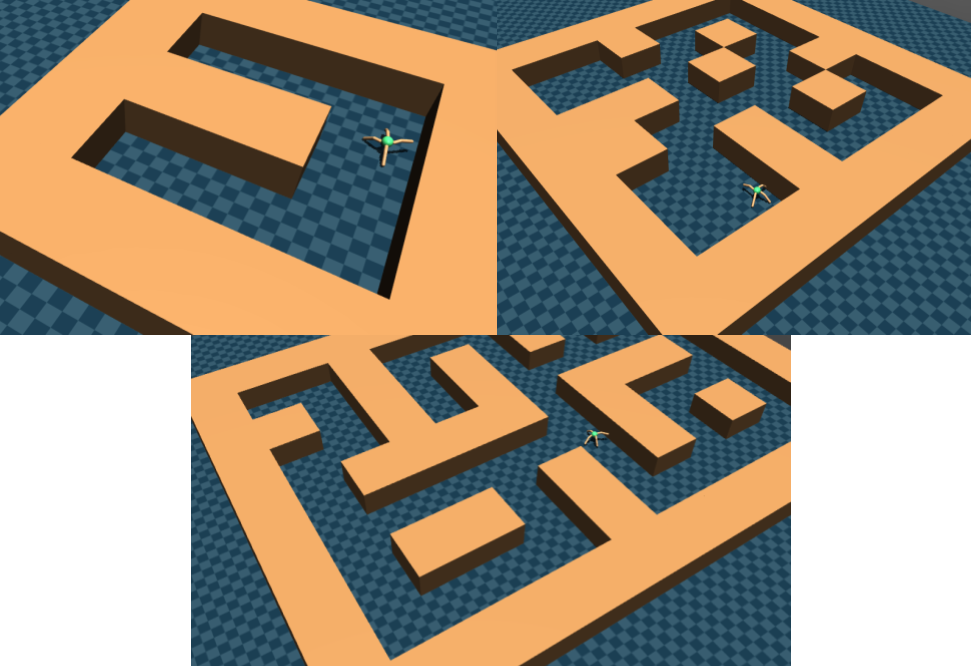
\includegraphics[width=0.17\textwidth]{chapters/cql/images/antmaze_all.png}
%     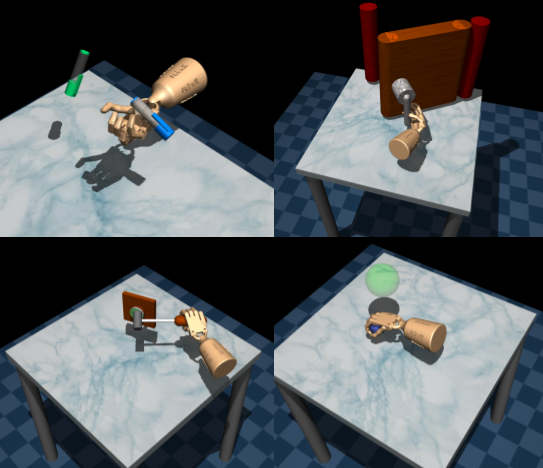
\includegraphics[width=0.97\linewidth]{chapters/cql/images/adroit_all.png}
%   \end{center}
%   \vspace{-21pt}
% \end{wrapfigure}
\textbf{Gym domains.} Results for the gym domains are shown in Table~\ref{table:mujoco}. The results for BEAR, BRAC, SAC, and BC are based on numbers reported by \citet{d4rl}. We find that across the board, on both the datasets generated by a single mediocre policy, marked as ``-medium'' and the datasets generated by mixing together experience from multiple policies (``-medium-replay'' and ``-medium-expert''), that are more likely to be encountered in practical problems, CQL outperforms prior methods.

% While CQL performs similarly to the best performing prior method when the offline dataset is constructed from a single RL policy, it significantly outperforms prior methods with complex data distributions, which are more indicative of real-world offline datasets~\citep{d4rl}.
%%SL.5.11: Well, if we're not going to show any of the AlgeaDICE results, maybe we shouldn't mention it before like this? We could add a sentence to the end of the first paragraph that describes all the prior methods and say something like: We also ran AlgeaDICE~\citep{} using code released by the authors, but were unable to get this method to improve over a random initialization on any of the tasks, as learning was unstable and diverged quickly.
% done
%%SL.5.11: In general, I think it would be best to break up the reported results into groups, and present them more slowly. For example, we could write the above paragraph something like this:
%The final performance of CQL($\mathcal{H}$) and each prior method on the D4RL tasks is shown in Table~\ref{table:something}. The first group of results is based on single-policy datasets for the MuJoCo gym benchmark environments: the ``-random'' and ``-medium'' datasets for HalfCheetah, Walker2D, and Hopper. These datsets are produced by either a random policy, or a medium-reward policy, respectively (see \citet{d4rl} for details). On these single-policy datasets, CQL matches or exceeds the best prior methods, but by a small margin. However, on the datasets that combine multiple policies (``-mixed,'' ``medium-expert,'' ``-random-expert''), prior methods generally perform substantially worse. Such mixed datasets are likely to be more common in real-world applications of offline RL, where training data might come from a variety of sources. CQL outperforms prior methods in these settings, on all three environments, in some cases by as much as 2-4x.
%%SL.5.11: You might want to also group the results in the tables/plots based on these groupings


% & halfcheetah-random & 100.0 & 2.1 & 30.5 & 25.5 & 23.5 & 28.1\\
% & walker2d-random & 100.0 & 1.6 & 4.1 & 6.7 & 0.8 & 0.5\\
% & hopper-random & 100.0 & 9.8 & 11.3 & 9.5 & 11.1 & 12.0\\
% & halfcheetah-medium & 100.0 & 36.1 & -4.3 & 38.6 & 44.0 & 45.5\\
% & walker2d-medium & 100.0 & 6.6 & 0.9 & 33.2 & 72.7 & 81.3\\
% & hopper-medium & 100.0 & 29.0 & 0.8 & 47.6 & 31.2 & 32.3\\
% & halfcheetah-medium-replay & 100.0 & 38.4 & -2.4 & 36.2 & 45.6 & 45.9\\
% & walker2d-medium-replay & 100.0 & 11.3 & 1.9 & 10.8 & -0.3 & 0.9\\
% & hopper-medium-replay & 100.0 & 11.8 & 3.5 & 25.3 & 0.7 & 0.8\\
% & halfcheetah-medium-expert & 100.0 & 35.8 & 1.8 & 51.7 & 43.8 & 45.3\\
% & walker2d-medium-expert & 100.0 & 6.4 & -0.1 & 26.0 & 3.1 & 66.6\\
% & hopper-medium-expert & 100.0 & 111.9 & 1.6 & 4.0 & 1.1 & 0.8\\
% %%%%%%%%%%%%%% TABLE %%%%%%%%%%%%%%%%%%%%%%
% \begin{table*}[h]
% \centering
% \small
% \begin{tabular}{l|r|r|r|r|r|r||r}
% \hline
% \textbf{Task Name} & \textbf{BC} & \textbf{SAC} & \textbf{BCQ} & \textbf{BEAR} & \textbf{BRAC-p} & \textbf{BRAC-v} & \textbf{CQL($\mathcal{H}$)}\\ \hline
% halfcheetah-random & -17.9 & 3502.0 & -2.1 & 2885.6 & 2641.0 & 3207.3 & \textbf{4524.7} \\
% halfcheetah-medium &  4196.4 & -808.6 & 4117.0 & 4508.7 & \textbf{5178.2} & \textbf{5365.3} & \textbf{5281.6} \\
% halfcheetah-mixed &  4492.1 & -581.3 & 3377.2 & 4211.3 & \textbf{5384.7} & \textbf{5413.8} & \textbf{5476.3}\\
% halfcheetah-medium-expert &  4169.4 & -55.7 &  7415.6 & 6132.5 & 5156.0 & 5342.4 & \textbf{9025.0}\\
% halfcheetah-random-expert &  -113.1 & 6298.7 & 7161.3 & 2768.8 & 3465.2 & -9.55 & \textbf{7951.9}\\ 
% \hline
% walker2d-random & 73.0 & 192.0 & 266.9 & 307.6 & 38.4 & 23.9 & \textbf{323.1}\\
% walker2d-medium & 304.8 & 44.2 & 881.7 & 1526.7 & 3341.1 & \textbf{3734.4} & \textbf{3801.4} \\
% walker2d-mixed & 518.6 & 87.8 & 384.6 & 495.3 & -11.5 & 44.5 & \textbf{1391.0} \\
% walker2d-medium-expert & 297.0 & -5.1 & 876.7 & 1193.6 & 141.7 & 3058.9 & \textbf{4348.1} \\
% walker2d-random-expert & 33.5 & 37.1 &  & 88.9 & 12.1 & 124.9 & \textbf{4245.8} \\
% \hline
% hopper-random & 299.4 & 347.7 & 274.7 & 289.5 & \textbf{341.0} & \textbf{370.5} & \textbf{355.2} \\
% hopper-medium & 923.5 & 5.7 & 1186.7 & 1527.9 & 994.8 & 1030.0 & \textbf{2403.1}\\
% hopper-mixed & 364.4 & 93.3 & 491.3 & 802.7 & 2.0 & 5.3 & \textbf{2267.9}\\
% hopper-medium-expert & \textbf{3621.2} & 32.9 & 2146.8 & 109.8 & 16.0 & 5.1 & \textbf{3699.1}\\
% \hline
% % ant-random & & & & & & & 932.4\\
% % ant-medium & & & & & & & 3325.4 \\
% % ant-mixed & & & & & & & 2973.8\\
% % ant-medium-expert & & & & & & & 3400.1 \\
% % ant-random-expert & & & & & & & 2309.3\\
% % \hline
% \end{tabular}
% \caption{{\footnotesize Performance of CQL and prior methods on gym MuJoCo tasks from D4RL. Observe that CQL performs similarly to the best prior method with simple datasets generated from a single RL policy, and greatly outperforms prior methods with mixed datasets.}}
% \label{table:mujoco}
% \normalsize
% \end{table*}
% %%SL.5.11: Maybe show some pictures of these tasks and the adroit and maze tasks, for readers that aren't familiar?
% % Yes I can add these, but i am concerned about too much space utilization
%%%%%%%%%%%%%%%%%%%%%%%%%%%%
% \begin{figure*}
% \centering
% 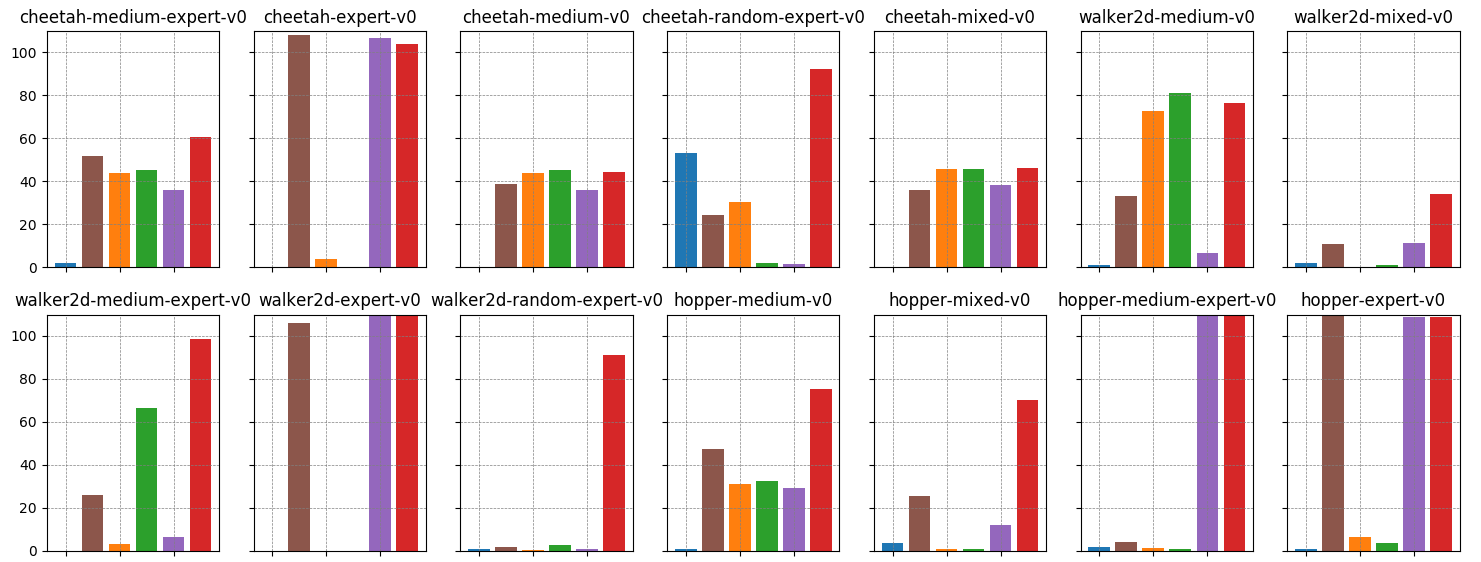
\includegraphics[width=0.99\linewidth]{chapters/cql/images/mujoco_results_v1.png}
% \caption{{\footnotesize Performance of CQL and prior methods on gym MuJoCo tasks from D4RL reported as a normalized score. Observe that CQL performs similarly to the best prior method with simple datasets generated from a single RL policy, and greatly outperforms prior methods with mixed datasets.}}
% \end{figure*}
    % 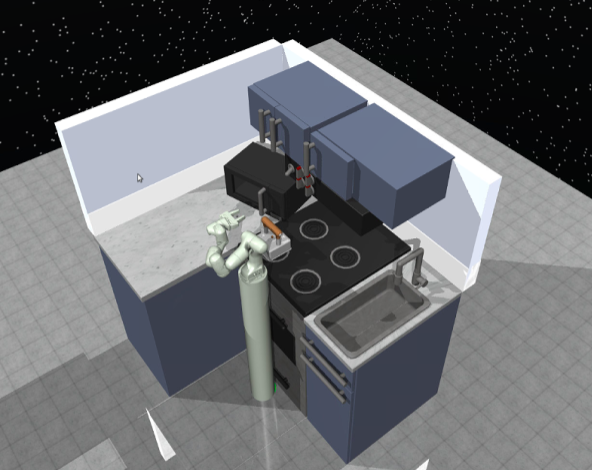
\includegraphics[width=0.9\linewidth]{chapters/cql/images/adept_franka_kitchen.png}

%% adroit tasks
\textbf{Adroit tasks.} The more complex Adroit~\citep{rajeswaran2018dapg} tasks in D4RL require controlling a 24-DoF robotic hand, using limited data from human demonstrations. These tasks are
substantially more difficult than the gym tasks in terms of both the dataset composition and high dimensionality. Prior offline RL methods generally struggle to learn meaningful behaviors on 
these tasks, and the strongest baseline is BC. As shown in Table~\ref{table:adroit_antmaze}, CQL variants are the only methods that improve over BC, attaining scores that are \textbf{2-9x} those of the next best offline RL method. CQL($\rho$) with $\rho = \hat{\policy}^{k-1}$ (the previous policy) outperforms CQL($\mathcal{H}$) on a number of these tasks, due to the higher action dimensionality resulting in higher variance for the CQL($\mathcal{H}$) importance weights. 
% Both variants outperform prior methods.
%%AK.5.23: need to say something about the CQL(rho) variant doing better -- which is due to importance sampling, but we never really talk about importance sampling so far.

\begin{table}[H]
\captionsetup{font=small}
\vspace{-1pt}
\centering
%\scriptsize
\fontsize{8}{8}\selectfont
\resizebox{0.99\textwidth}{!}{
\begin{tabular}{l|l|r|r|r|r|r||r|r}
\hline
\textbf{Domain} & \textbf{Task Name} & \textbf{BC} & \textbf{SAC} & \textbf{BEAR} & \textbf{BRAC-p} & \textbf{BRAC-v} & \textbf{CQL($\mathcal{H}$)} & \textbf{CQL($\rho$)}\\ \hline
% \multirow{3}*{Maze2D}
% & maze2d-umaze &  3.8 & 88.2 & 3.4 & 4.7 & -14.6\\
% & maze2d-medium &  30.3 & 26.1 & 29.0 & 32.4 & 149.0\\
% & maze2d-large &  5.0 & -1.9 & 4.6 & 10.4 & 150.0\\
% \hline
\multirow{6}*{AntMaze}
& antmaze-umaze-v2 & 54.6 & 0.0 & {73.0} & 50.0 & 70.0 & \textbf{94.0} & - \\
& antmaze-umaze-diverse-v2  & 45.6 & 0.0 & 61.0 & 40.0 & 70.0 & {47.3} & - \\
& antmaze-medium-play-v2  & 0.0 & 0.0 & 0.0 & 0.0 & 0.0 & \textbf{62.4} & - \\
& antmaze-medium-diverse-v2  & 0.0 & 0.0 & 8.0 & 0.0 & 0.0 & \textbf{74.3}  & - \\
& antmaze-large-play-v2 & 0.0 & 0.0 & 0.0 & 0.0 & 0.0 & \textbf{34.2} & - \\
& antmaze-large-diverse-v2 & 0.0 & 0.0 & 0.0 & 0.0 & 0.0 & \textbf{40.7} & - \\
\hline
& \textbf{Total (antmazes)} & 100.2 & 0.0 & - & - & - & \textbf{352.9} & -\\
\hline
\multirow{8}*{Adroit}
& pen-human  & 34.4 & 6.3 & -1.0 & 8.1 & 0.6 & 37.5 & \textbf{55.8}\\
& hammer-human & 1.5 & 0.5 & 0.3 & 0.3 & 0.2 & \textbf{4.4} & {2.1}\\
& door-human & 0.5 & 3.9 & -0.3 & -0.3 & -0.3 & \textbf{9.9} & \textbf{9.1} \\
& relocate-human & 0.0 & 0.0 & -0.3 & -0.3 & -0.3 & 0.20 & \textbf{0.35}\\
& pen-cloned  & \textbf{56.9} & 23.5 & 26.5 & 1.6 & -2.5 & 39.2 & 40.3\\
& hammer-cloned & 0.8 & 0.2 & 0.3 & 0.3 & 0.3 & 2.1 & \textbf{5.7} \\
& door-cloned & -0.1 & 0.0 & -0.1 & -0.1 & -0.1 & 0.4 & \textbf{3.5}\\
& relocate-cloned & \textbf{-0.1} & -0.2 & -0.3 & -0.3 & -0.3 & \textbf{-0.1} & \textbf{-0.1}\\
\hline
\multirow{3}*{Kitchen}
& kitchen-complete & 33.8 & 15.0 & 0.0 & 0.0 & 0.0 & \textbf{43.8} & 31.3\\
& kitchen-partial & 33.8 & 0.0 & 13.1 & 0.0 & 0.0 & \textbf{49.8} & \textbf{50.1} \\
& kitchen-undirected & 47.5 & 2.5 & 47.2 & 0.0 & 0.0 & \textbf{51.0} & \textbf{52.4} \\ \hline
\end{tabular}
}
\vspace{0.1cm}
\caption{\label{table:adroit_antmaze}{Normalized scores of all methods on AntMaze, Adroit, and kitchen domains from D4RL, averaged across 4 seeds. On the harder mazes, CQL is the \textit{only} method that attains non-zero returns, and is the only method to outperform simple behavioral cloning on Adroit tasks with human demonstrations.
We observed that the CQL($\rho$) variant, which avoids importance weights, trains more stably, with no sudden fluctuations in policy performance over the course of training, on the higher-dimensional Adroit tasks.}}
\normalsize
\end{table}

\textbf{AntMaze.} 
These tasks require composing parts of suboptimal trajectories to form more optimal policies for reaching goals on a MuJoco Ant robot. 
Prior methods make some progress on the simpler U-maze, but only CQL is able to make meaningful progress  
%% adroit tasks
on the much harder medium and large mazes, outperforming prior methods.
%, achieving nearly \textbf{2-5x} higher return as compared to prior methods.

% \begin{wrapfigure}{r}{0.3\textwidth}
%   \vspace{-25pt}
%   \begin{center}
%   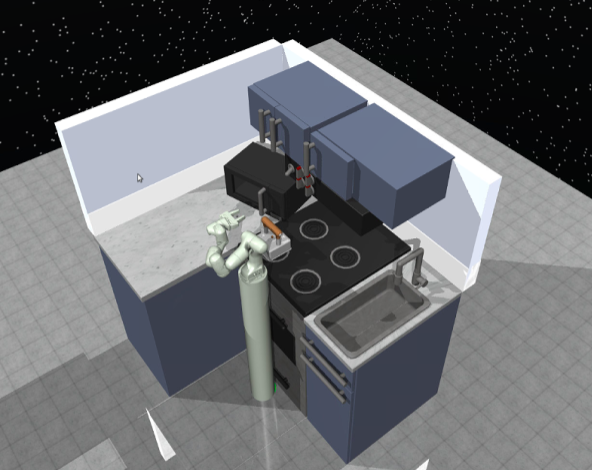
\includegraphics[width=0.99\linewidth]{chapters/cql/images/adept_franka_kitchen.png}
%   \end{center}
%   \vspace{-20pt}
% \end{wrapfigure}
\textbf{Kitchen tasks.} Next, we evaluate CQL on the Franka kitchen domain~\citep{gupta2019relay} from D4RL~\citep{d4rl_repo}.
The goal is to control a 9-DoF robot to manipulate multiple objects (microwave, kettle, etc.) \textit{sequentially}, in a single episode to reach a desired configuration, with only sparse 0-1 completion reward for every object that attains the target configuration. These tasks are especially challenging, since they require composing parts of trajectories, precise long-horizon manipulation, and handling human-provided teleoperation data. As shown in Table~\ref{table:adroit_antmaze}, CQL outperforms prior methods in this setting, and is the only method that outperforms behavioral cloning, attaining over \textbf{40\%} success rate on all tasks.



% \begin{table*}[h]
% \centering
% \small
% \begin{tabular}{l|r|r|r|r|r|r|r|r}
% \hline
% \textbf{Task Name} & \textbf{SAC} & \textbf{BC} & \textbf{SAC-off} & \textbf{BEAR} & \textbf{BRAC-p} & \textbf{BRAC-v} & \textbf{CQL($\mathcal{H}$)} & \textbf{CQL($\rho$)}\\ \hline
% ant-umaze & 0.0 & 0.7 & 0.0 & 0.7 & 0.5 & 0.7 & \textbf{0.74} & \\
% ant-umaze-diverse & 0.0 & 0.6 & 0.0 & 0.6 & 0.4 & 0.7 & \textbf{0.79} & \\
% ant-medium-play & 0.0 & 0.0 & 0.0 & 0.0 & 0.0 & 0.0 & \textbf{0.54 } & \\
% ant-medium-diverse & 0.0 & 0.0 & 0.0 & 0.0 & 0.0 & 0.0 & \textbf{0.53} & \\
% ant-large-play & 0.0 & 0.0 & 0.0 & 0.0 & 0.0 & 0.0 & \textbf{0.20} & \\
% ant-large-diverse & 0.0 & 0.0 & 0.0 & 0.0 & 0.0 & 0.0 & \textbf{0.19} & \\
% \hline
% pen-human & 739.3 & 1121.9 & 284.8 & 66.3 & 339.0 & 114.7 & \textbf{1367.5} & \\
% hammer-human & -248.7 & -82.4 & -214.2 & -242.0 & -239.7 & -243.8 & \textbf{1098.1} & \\
% door-human & -61.8 & -41.7 & 57.2 & -66.4 & -66.5 & -66.4 & \textbf{273.0} & \\
% relocate-human & -13.7 & -5.6 & -4.5 & -18.9 & -19.7 & -19.7 & \textbf{5.7} & \\
% pen-cloned & \\
% hammer-cloned & \\
% door-cloned & \\
% relocate-cloned & \\
% \hline
% mini-kitchen-MKLS & \\
% kitchen-MKLS & \\
% kitchen-MKBL & \\
% \hline
% \end{tabular}
% \caption{{\footnotesize Performance of CQL and prior methods on AntMaze, Adroit and kitchen tasks from D4RL. Observe that CQL outperforms prior methods on the simpler U-shaped maze and is the \textit{only} method that is able to obtain non-zero performance on the harder, medium-sized maze. CQL is the only method that achieves a positive return on adroit tasks with human demonstrations.}}
% \label{table:adroit_antmaze}
% \normalsize
% \end{table*}
% \multirow{12}*{Adroit}
% & pen-human & 739.3 & 1121.9 & 284.8 & 66.3 & 339.0 & 114.7\\
% & pen-cloned & 739.3 & 1791.8 & 797.6 & 885.4 & 143.4 & 22.2\\
% & pen-expert & 739.3 & 2633.7 & 277.4 & 3254.1 & -7.8 & 6.4\\
% & hammer-human & -248.7 & -82.4 & -214.2 & -242.0 & -239.7 & -243.8\\
% & hammer-cloned & -248.7 & -175.1 & -244.1 & -241.1 & -236.7 & -236.9\\
% & hammer-expert & -248.7 & 16140.8 & 3019.5 & 16359.7 & -241.4 & -241.1\\
% & door-human & -61.8 & -41.7 & 57.2 & -66.4 & -66.5 & -66.4\\
% & door-cloned & -61.8 & -60.7 & -56.3 & -60.9 & -58.7 & -59.0\\
% & door-expert & -61.8 & 969.4 & 163.8 & 2980.1 & -66.4 & -66.6\\
% & relocate-human & -13.7 & -5.6 & -4.5 & -18.9 & -19.7 & -19.7\\
% & relocate-cloned & -13.7 & -10.1 & -16.1 & -17.6 & -19.8 & -19.4\\
% & relocate-expert & -13.7 & 4289.3 & -18.2 & 4173.8 & -20.6 & -21.4\\
% \hline
% \multirow{12}*{Gym}
% & halfcheetah-random & 12135.0 & -17.9 & 3502.0 & 2885.6 & 2641.0 & 3207.3\\
% & halfcheetah-medium & 12135.0 & 4196.4 & -808.6 & 4508.7 & 5178.2 & 5365.3\\
% & halfcheetah-mixed & 12135.0 & 4492.1 & -581.3 & 4211.3 & 5384.7 & 5413.8\\
% & halfcheetah-medium-expert & 12135.0 & 4169.4 & -55.7 & 6132.5 & 5156.0 & 5342.4\\
% & walker2d-random & 4592.3 & 73.0 & 192.0 & 307.6 & 38.4 & 23.9\\
% & walker2d-medium & 4592.3 & 304.8 & 44.2 & 1526.7 & 3341.1 & 3734.4\\
% & walker2d-mixed & 4592.3 & 518.6 & 87.8 & 495.3 & -11.5 & 44.5\\
% & walker2d-medium-expert & 4592.3 & 297.0 & -5.1 & 1193.6 & 141.7 & 3058.9\\
% & hopper-random & 3234.3 & 299.4 & 347.7 & 289.5 & 341.0 & 370.5\\
% & hopper-medium & 3234.3 & 923.5 & 5.7 & 1527.9 & 994.8 & 1030.0\\
% & hopper-mixed & 3234.3 & 364.4 & 93.3 & 802.7 & 2.0 & 5.3\\
% & hopper-medium-expert & 3234.3 & 3621.2 & 32.9 & 109.8 & 16.0 & 5.1\\
% \hline

%%SL.5.24: Consider deleting subsection headings in the whole experiments section. They really don't add much, and you can save some space.
%\subsection{Offline Image-Based RL on the Arcade Learning Environment}
\textbf{Offline RL on Atari games\footnote{Results for CQL on more Atari games, with varied dataset compositions can be found in Appendix F of DR3 (Kumar et al. ICLR 2022), available at the following arXiv URL: \url{https://arxiv.org/abs/2112.04716}}.} Lastly, we evaluate a discrete-action Q-learning variant of CQL (Algorithm~\ref{alg:practical_alg}) on offline, image-based Atari games~\citep{bellemare2013arcade}. We compare CQL to REM~\citep{agarwal2019optimistic} and QR-DQN~\citep{dabney2018distributional} on the five Atari tasks (Pong, Breakout, Qbert, Seaquest and Asterix) that are evaluated in detail by \citet{agarwal2019optimistic}, using the dataset released by the authors. 
% We were not able to reproduce the QR-DQN and REM results on Asterix using the official implementation and data from \citet{agarwal2019optimistic}, and no method was able to perform well on the provided data for this task, but we include the scores in Table~\ref{table:atari_reduced_size}.

\begin{figure*}[h]
\vspace{-12pt}
\begin{center}
  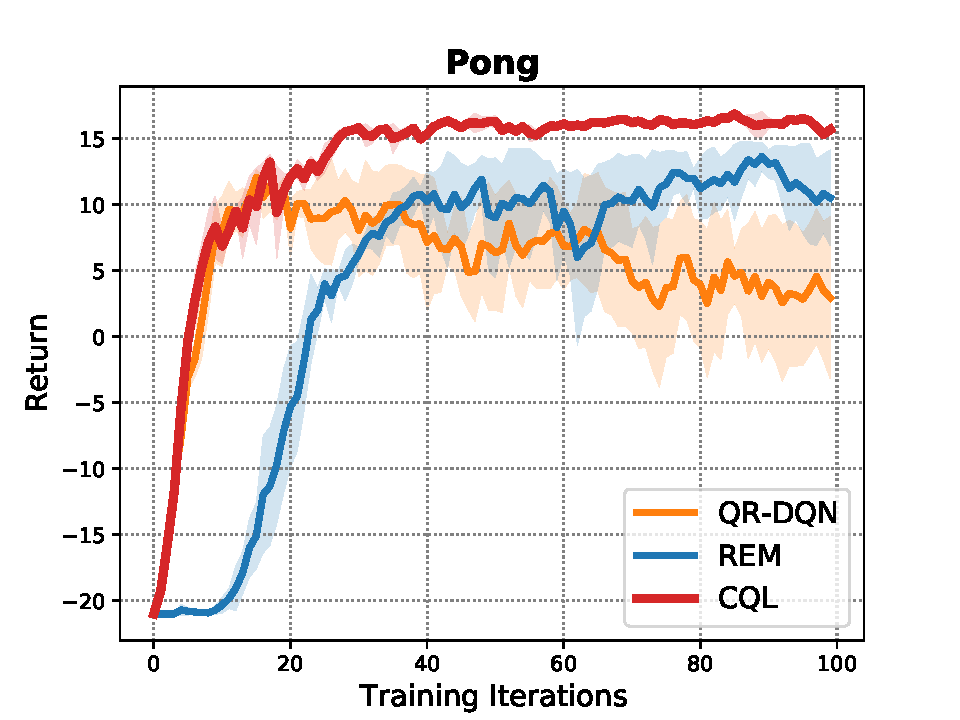
\includegraphics[width=0.23\linewidth]{chapters/cql/images/pong.pdf}  
  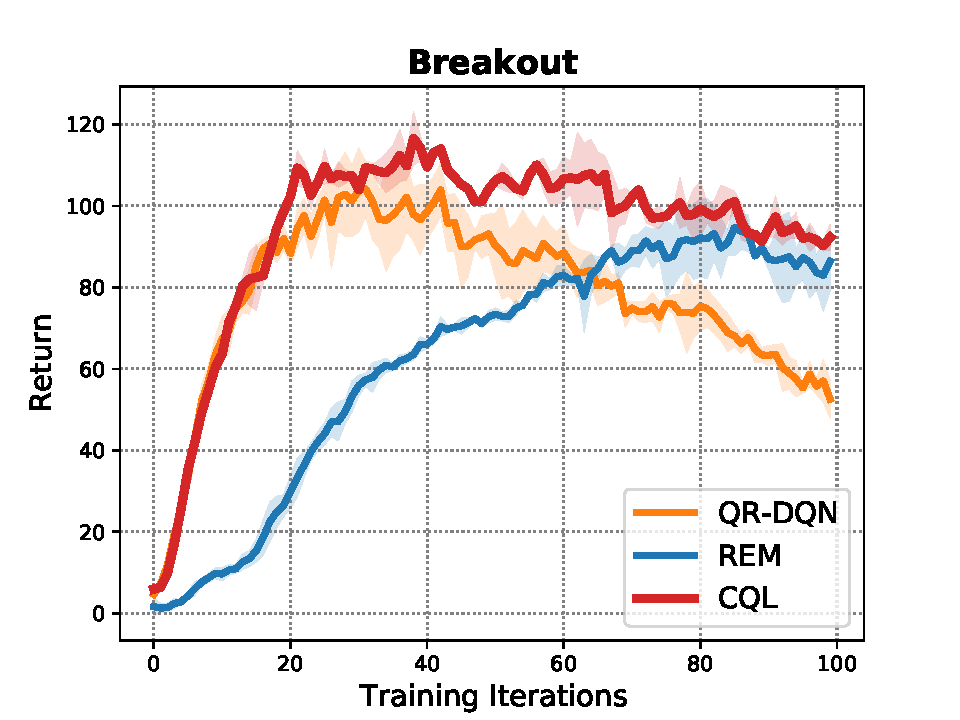
\includegraphics[width=.23\linewidth]{chapters/cql/images/breakout.pdf}  
  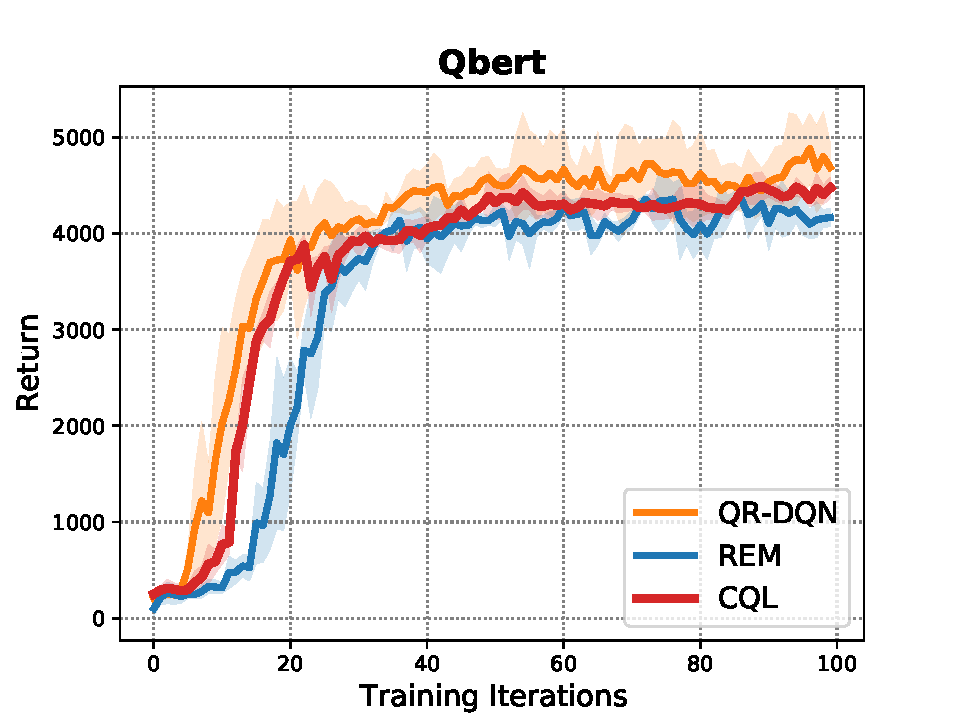
\includegraphics[width=.23\linewidth]{chapters/cql/images/qbert.pdf}  
  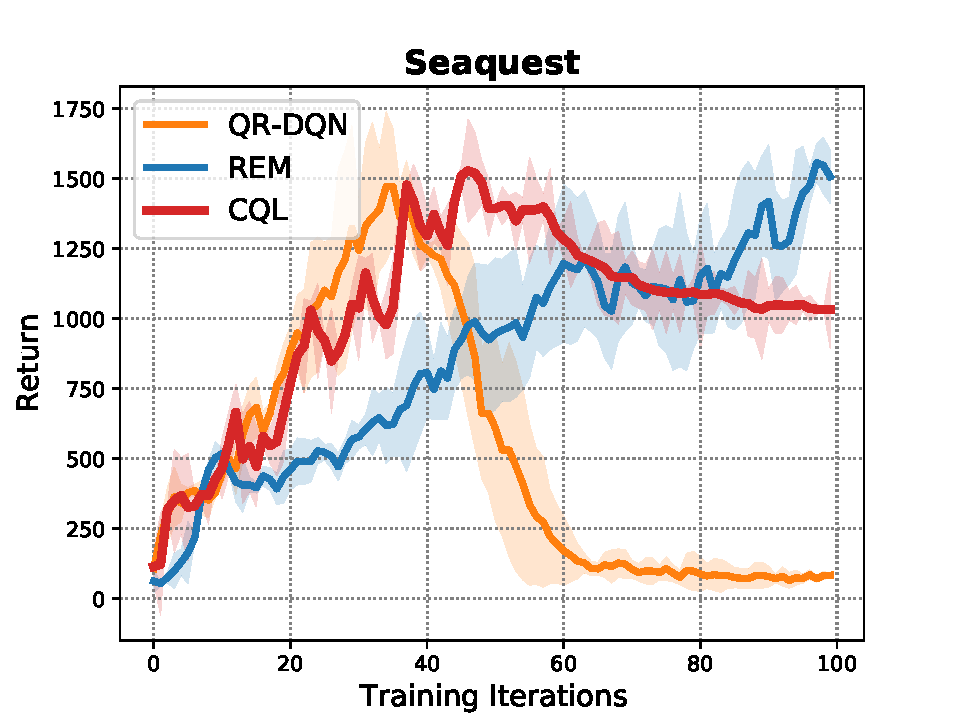
\includegraphics[width=.23\linewidth]{chapters/cql/images/seaquest.pdf}  
\end{center}
\vspace{-4pt}
\caption{\label{fig:cql_20m_atari}{\footnotesize Performance of CQL, QR-DQN and REM as a function of training steps (x-axis) in setting \textbf{(1)} when provided with only the first 20\% of the samples of an online DQN run. Note that CQL is able to learn stably on 3 out of 4 games, and its performance does not degrade as steeply as QR-DQN on Seaquest.}}
\vspace{-10pt}
\end{figure*}
Following the evaluation protocol of \citet{agarwal2019optimistic}, we evaluated on two types of datasets, both of which were generated from the DQN-replay dataset, released by~\citep{agarwal2019optimistic}:
\textbf{(1)} a dataset consisting of the first 20\% of the samples observed by an online DQN agent and 
\textbf{(2)} datasets consisting of only 1\%  and 10\% of all samples observed by an online DQN agent (Figures 6 and 7 in \citep{agarwal2019optimistic}). In setting \textbf{(1)}, shown in Figure~\ref{fig:cql_20m_atari}, CQL generally achieves similar or better performance throughout as QR-DQN and REM. When only using only 1\% or 10\% of the data, in setting \textbf{(2)} (Table~\ref{table:atari_reduced_size}),  CQL substantially outperforms REM and QR-DQN, especially in the harder 1\% condition, achieving \textbf{36x} and \textbf{6x} times the return of the best prior method on Q*bert and Breakout, respectively.

%AK: TODO (aviral): revisit this if we can't get seaquest to work -- Seaquest is almost maxed out, need to decide on what to say here?
\begin{table}
\captionsetup{font=small}
    \centering
    % \vspace{-7pt}
    \fontsize{8}{8}\selectfont
    \resizebox{0.56\textwidth}{!}{\begin{tabular}{l|r|r||r}
    \hline
        \textbf{Task Name} & \textbf{QR-DQN} & \textbf{REM} & \textbf{CQL($\mathcal{H}$)} \\
        \hline
         Pong (1\%) & -13.8 & -6.9 & \textbf{19.3} \\
         Breakout & 7.9 & 11.0 & \textbf{61.1} \\
         Q*bert & 383.6 & 343.4 & \textbf{14012.0} \\
         Seaquest & 672.9 & 499.8 & \textbf{779.4} \\
         Asterix  & 166.3 & 386.5 & \textbf{592.4}\\
         \hline
         \hline
         Pong (10\%) & 15.1 & 8.9 & \textbf{18.5} \\
         Breakout & 151.2 & 86.7 & \textbf{269.3} \\
         Q*bert & 7091.3 & 8624.3 & \textbf{13855.6}\\
         Seaquest & 2984.8 & \textbf{3936.6} & 3674.1 \\
         Asterix & \textbf{189.2} & 75.1 & 156.3 \\
         \hline
    \end{tabular}}
    % \vspace{-4pt}
    \caption{\footnotesize{CQL, REM and QR-DQN in setting \textbf{(1)} with 1\% data (top), and 10\% data (bottom). CQL outperforms prior methods with 1\% data, and usually attains better performance with 10\% data.}}
    \normalsize
    \label{table:atari_reduced_size}
\end{table}
% \let\thefootnote\relax\footnote{{\small *Neither CQL nor any prior method, including REM, attains non-trivial performance on Asterix. When using exactly the same dataset and implementation provided by \citet{agarwal2019optimistic}, we were unable to reproduce the numbers reported in~\citep{agarwal2019optimistic} for QR-DQN and REM. }}

% \begin{table}[h]
% \captionsetup{font=small}
%     \centering
%     \vspace{-10pt}
%     \fontsize{8}{8}\selectfont
%     \begin{tabular}{l|r|r|r|||r|r|r}
%     \hline
%         \textbf{Task Name} & \textbf{QR-DQN} & \textbf{REM} & \textbf{CQL($\mathcal{H}$)}  & \textbf{QR-DQN} & \textbf{REM} & \textbf{CQL($\mathcal{H}$)}  \\
%         \hline
%          Pong & 3.0 & 6.0 & \textbf{19.3} & 16.7 & 16.8 & \textbf{18.5} \\
%          Breakout & 7.8 & 9.2 & \textbf{61.1} & 176.0 & 96.0 & \textbf{269.3} \\
%          Q*bert & 500.0 & 500.0 & \textbf{14012.0}& 11201.8 & 8070.2 & \textbf{13855.6}\\
%          Seaquest & 480.2 & 390.1 & \textbf{779.4} & 3300.0 & \textbf{4290.4} & 3674.1 \\
%          %%SL.5.30: Something is wrong! This footnote doesn't seem to actually show up in the paper!!
%          Asterix\footnote{No method (CQL or prior methods, REM and QR-DQN, were able to attain non-trivial performance on this game using the dataset provided by \citet{agarwal2019optimistic}} & 166.3 & 386.5 & \textbf{592.4} & 189.2 & 75.1 & 156.3 \\
%          \hline
%     \end{tabular}
%     \caption{{CQL, REM and QR-DQN in setting \textbf{(1)} with 1\% data (left), and 10\% data (right). CQL drastically outperforms prior methods with 1\% data, and usually attains better performance with 10\%.}}
%     \normalsize
%     \label{table:atari_reduced_size}
% \footnote{No method (CQL or prior methods, REM and QR-DQN, were able to attain non-trivial performance on this game using the dataset provided by \citet{agarwal2019optimistic}}
% \end{table}

\textbf{Analysis of CQL.} Finally, we perform empirical evaluation to verify that CQL indeed lower-bounds the value function, thus verifying Theorems~\ref{thm:cql_underestimates}, Appendix~\ref{thm:policy_eval_func_approx} empirically. To this end, we estimate the average value of the learned policy predicted by CQL, $\E_{\bs \sim \mathcal{D}}[\hat{V}^k(\bs)]$, and report the difference against the actual discounted return of the policy $\policy^{k}$ in Table~\ref{table:cql_lower_bound}. We also estimate these values for baselines, including the minimum predicted Q-value under an ensemble~\citep{haarnoja,fujimoto2018addressing}
%%SL.5.30: Maybe reference some papers that do this, like TD3 and REM?
of Q-functions with varying ensemble sizes, which is a standard technique to prevent overestimed Q-values~\citep{fujimoto2018addressing,haarnoja,hasselt2010double} and BEAR~\citep{kumar2019stabilizing}, a policy constraint method. The results show that CQL learns a lower bound for all three tasks, whereas the baselines are prone to overestimation. We also evaluate a variant of CQL that uses Equation~\ref{eqn:objective_1}, and observe that the resulting values are lower (that is, underestimate the true values) as compared to CQL($\mathcal{H}$). This provides empirical evidence that CQL($\mathcal{H}$) attains a tighter lower bound than the point-wise bound in Equation~\ref{eqn:objective_1}, as per Theorem~\ref{thm:cql_underestimates}. We also present an empirical analysis to show that Theorem~\ref{thm:gap_amplify}, that CQL is gap-expanding, holds in practice in Appendix~\ref{app:gap_amplify}, and present an ablation study on various design choices used in CQL in Appendix~\ref{app:cql_additional_results}.

\begin{table}[h]
\captionsetup{font=small}
\centering
    \fontsize{8}{8}\selectfont
    \resizebox{0.99\textwidth}{!}{\begin{tabular}{l|r|r||r|r|r|r|r}
    \hline
        \textbf{Task Name} & \textbf{CQL($\mathcal{H})$} & \textbf{CQL (Eqn.~\ref{eqn:objective_1})} & \textbf{Ensemble(2)}  & \textbf{Ens.(4)} & \textbf{Ens.(10)} & \textbf{Ens.(20)} & \textbf{BEAR} \\
        \hline
        %%SL.5.30: bold the best result that is still a bound
        hopper-medium-expert & \textbf{-43.20} & -151.36 & 3.71e6 & 2.93e6 & 0.32e6 & 24.05e3 & 65.93 \\
        hopper-mixed & \textbf{-10.93} & -22.87 & 15.00e6 &  59.93e3 & 8.92e3 & 2.47e3 & 1399.46 \\
        hopper-medium & \textbf{-7.48} & -156.70 & 26.03e12 & 437.57e6 & 1.12e12 & 885e3 & 4.32 \\
        %%SL.5.30: I would recommend using scientific notation (e.g., e6 or $\times 10^6$) instead of "M" or "T"
        \hline
    \end{tabular}}
    \caption{{Difference between predicted policy values and the true policy value for CQL, a variant of CQL that uses Equation~\ref{eqn:objective_1}, the minimum of an ensemble of varying sizes, and BEAR~\citep{kumar2019stabilizing} on three D4RL datasets. CQL is the only method that lower-bounds the actual return (i.e., has negative differences), and CQL($\mathcal{H})$ is much less conservative than CQL (Eqn.~\ref{eqn:objective_1}).}}
    \normalsize
    \vspace{-10pt}
    \label{table:cql_lower_bound}
\end{table}



%%AK.5.23: Commenting out this for now, discussion in the email. Basically we are not doing great here especially with the right way of using the Q-values for computing policy return. It is conservative, but it is too conservative in 4/8 cases (like the method outputs 153.4 as the return, but the actual return is 276). I think that if we believe that the other story is storng enough, we should probably not have it.
% \subsection{Off-Policy Evaluation Experiments}

% %%SL.5.11: Can we start off with a little transition to explain why we're talking about this? E.g., something like: The core of CQL is a Q-function learning method that learns a lower bound on the true Q-function. This lower bound can be used to learn a better policy, or simply to evaluate an existing policy. In this section, we study this latter setting, applying CQL to the off-policy evaluation problem.
% % done
% CQL learns a Q-function such that the expected value of the policy under this learned Q-function lower-bounds the true policy value. In this section, we evaluate the performance of CQL for evaluating the performance of a pre-specified policy using pre-specified offline datasets on three continuous control domains: Hopper, HalfCheetah and Walker2d. In accordance with the setup in prior work~\citep{Zhang2020GenDICE}, our task is to evaluate the return of an expert SAC policy using data generated from a mixture of suboptimal policies. Thus, we use the medium-expert and mixed datasets from \citep{d4rl} that contain a diverse mixture of suboptimal policies as the offline datasets.

% We compare CQL to state-of-the-art prior method, GenDICE~\citep{zhang2019generalized}, in Table ??. Note that CQL learns conservative return estimates, that lower bound the actual discounted return of the target policy, thus empirically validating the theoretical insights discussed in Section~\ref{sec:policy_eval}. In contrast,  (One line about OTHER METHODS once we have numbers) \ak{TODO: put table.}


\vspace{-0.2cm}
\section{Model-Based Conservative Value Function Estimation}
\label{sec:combo_section}
\vspace{-0.2cm}

\begin{figure}[t!]
    \centering
    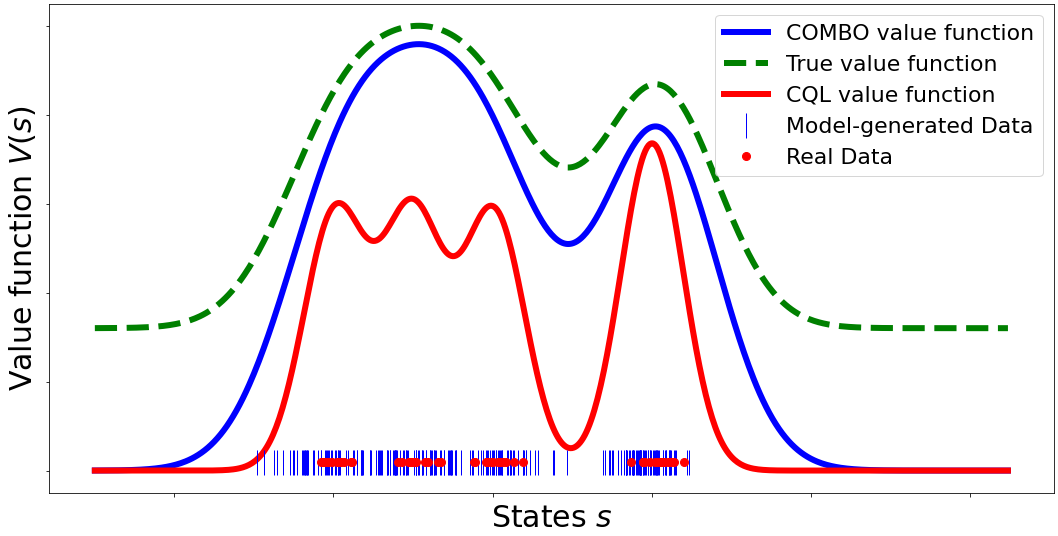
\includegraphics[width=0.5\textwidth]{chapters/combo/teaser_combo.png}
    \vspace*{-0.5cm}
    \caption{\footnotesize{COMBO learns a conservative value function by utilizing both the offline dataset as well as simulated data from the model. Crucially, COMBO does not require uncertainty quantification, and the value function learned by COMBO is a tighter lower-bound of the true value compared to CQL. This enables COMBO to steer the agent towards higher value states compared to CQL, which may steer towards sub-optimal states as illustrated in the figure.}}
    \vspace*{-0.6cm}
    \label{fig:combo_teaser}
\end{figure}

In Section~\ref{sec:cql_section}, we discussed conservative Q-learning, a model-free algorithm that learns conservative value functions on offline datasets. An alternative way to use offline data is to first attempt to estimate the dynamics of the underlying task, followed by training control policies via planning or explicit policy optimization. Empirically, in the standard RL problem setting, model-based RL algorithms have achieved better generalization~\citep{sutton1991dyna,janner2019mbpo}, especially in multi-task settings~\citep{yu2020mopo}. Specifically, one performant recipe for model-based RL is to utilize an estimated or learned dynamics model to generate data for a downstream model-free control pipeline, such as one based on Q-learning~\citep{janner2019mbpo}. 

Despite appealing properties of model-based RL, existing model-based methods still suffer from similar problems in the offline setting: any learned model of the environment dynamics is bound to make erroneous predictions on states or actions that are unlikely to appear within the support of the training dataset, and inevitably, downstream policy optimization will exploit these errors to produce policies that appear performant under the learned model, but fail to act reliably when deployed. To address this issue, existing offline model-based RL algorithms~\cite{kidambi2020morel, yu2020mopo} rely on precise quantifying uncertainty in predictions made by the learned dynamics model. However, as we show in Section~\ref{sec:uq}, obtaining calibrated uncertainty estimates can be extremely difficult, especially for complex datasets with deep network models.  
% A natural next step is to extend this approach to use dynamics models. By generating data, model-based reinforcement learning algorithms can achieve better generalization~\citep{sutton1991dyna,janner2019mbpo} and have demonstrated the ability to solve new tasks using the offline dataset~\cite{yu2020mopo}. 
% Most existing model-based algorithms learn a pessimistic dynamics model, which in turn induces a conservative estimate of the value function. 
% By generating data, model-based algorithms can achieve better generalization and e.g. have demonstrated the ability to solve new tasks using the offline dataset~\cite{yu2020mopo}.
% However, such algorithms rely crucially 
% Furthermore, these methods do not adapt the uncertainty estimates as the policy and value function change over the course of learning.
%%SL.1.31: The significance of this is not entirely clear (but I agree this is a true statement, and it's a nice observation, just that most readers won't get why this is important without more explanation)

To alleviate the need for calibrated uncertainty estimation, in this section, we develop a new model-based offline RL algorithm, building on conservative value estimation paradigm. Our approach, conservative offline model-based policy optimization (COMBO), retains the benefits of model-based algorithms while removing the reliance on uncertainty estimation. COMBO first learns a dynamics model using the offline dataset. Subsequently, it employs an actor-critic method where the value function is learned using both the offline dataset as well as synthetically generated data from the model. Crucially, this value function is trained via a variant of conservative optimization, that penalizes the value function on state-action tuples that are visited by the policy by simulating the learned model, but are not in the support of the offline dataset.
Using the theoretical tools from Section~\ref{sec:cql_section}, we theoretically show that for any policy, the Q-function learned with COMBO is a lower bound of the true Q-function, making it a good surrogate for policy optimization. 
We also theoretically show that the Q-function learned by COMBO represents a tighter lower bound of the true Q-function when the model bias is low compared to prior model-free algorithms like CQL~\cite{kumar2020conservative}.
Thus, as a consequence of optimizing a tighter lower bound, COMBO has the potential to learn higher rewarding policies compared to prior model-free algorithms. This is illustrated in Figure~\ref{fig:combo_teaser}.

Finally, in our experiments, we find that COMBO matches or exceeds the state-of-the-art results in commonly studied benchmark tasks for offline RL. Specifically, COMBO achieves the highest score in $9$ out of $12$ continuous control domains from the D4RL~\cite{fu2020d4rl} benchmark suite, while the next best algorithm achieves the highest score in only $3$ out of the $12$ domains. We also show that COMBO achieves the best performance in tasks that require out-of-distribution generalization and outperforms previous offline model-based RL methods on this image-based robotic manipulation task.%%CF: Need to also mention the generalization results and the vision results!
%%TY.2.3: added a sentence on the generalization and vision results. Rafael, feel free to also add the vision-based locomotion task to the sentence if we are going to include the walker results. 


%% Now adding material from COMBO paper
\subsection{Analysis: Uncertainty Calibration in Offline Model-Based RL}
\label{sec:uq}

\begin{figure}[t]
    \vspace{-0.5cm}
        \centering
        % 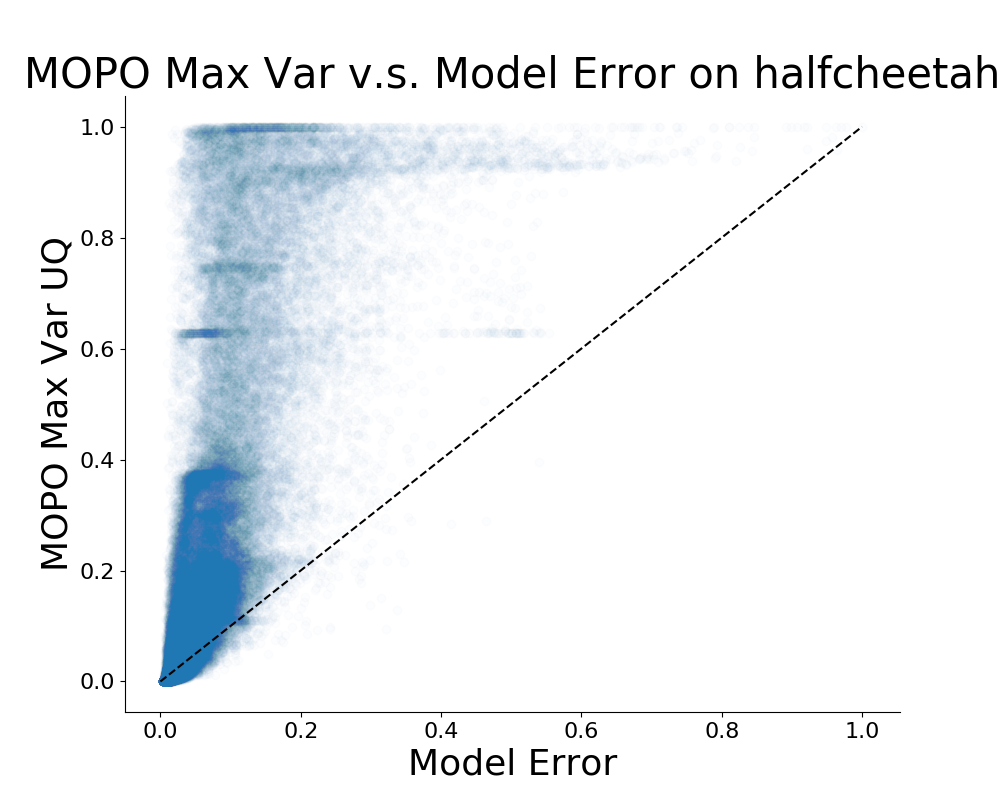
\includegraphics[width=0.47\linewidth]{halfcheetah_medium_corr_var_ood.png}
        % 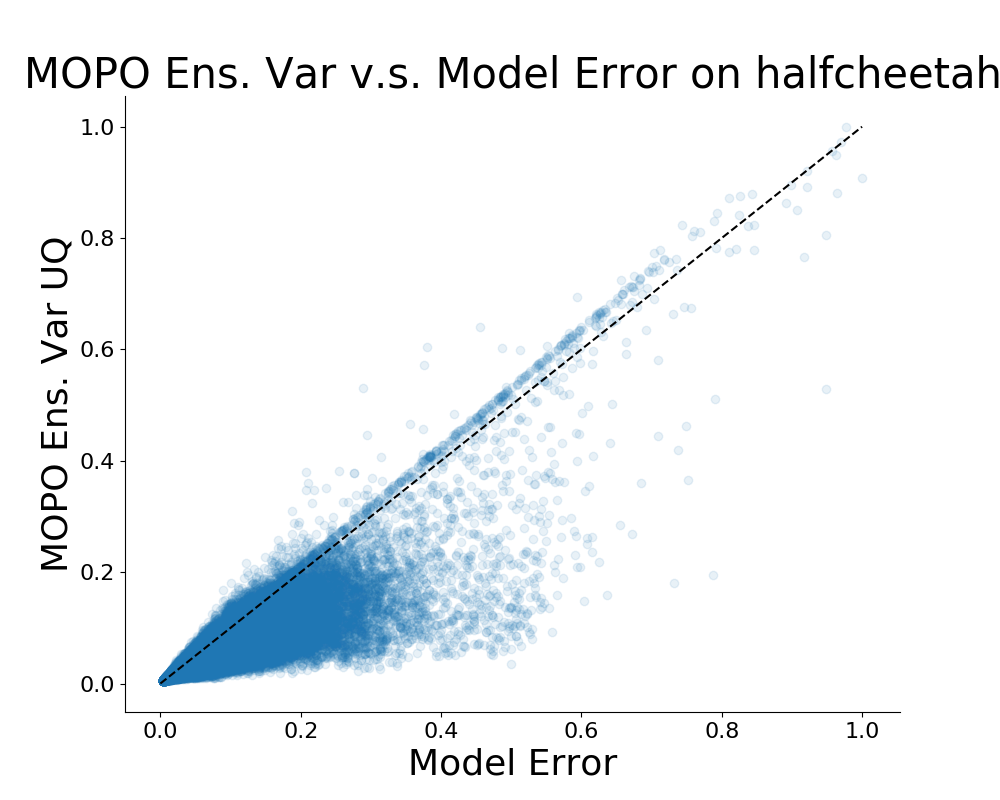
\includegraphics[width=0.47\linewidth]{halfcheetah_medium_corr_lip_ens_ood.png}
        % 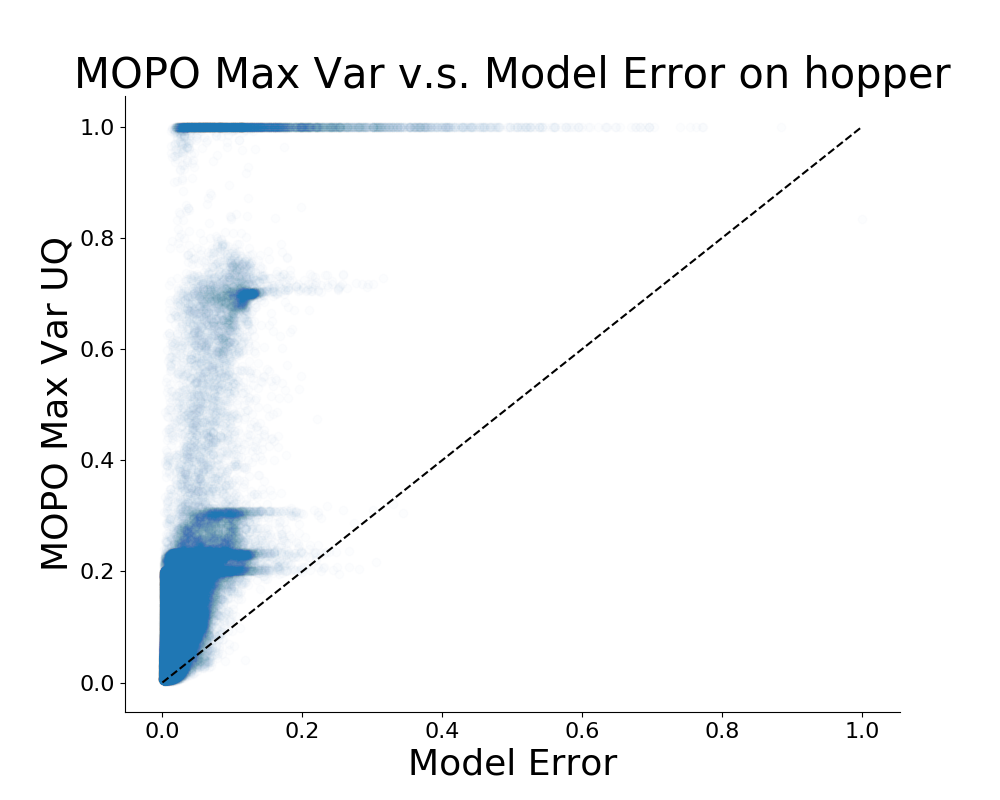
\includegraphics[width=0.47\linewidth]{hopper_medium_corr_var_ood.png}
        % 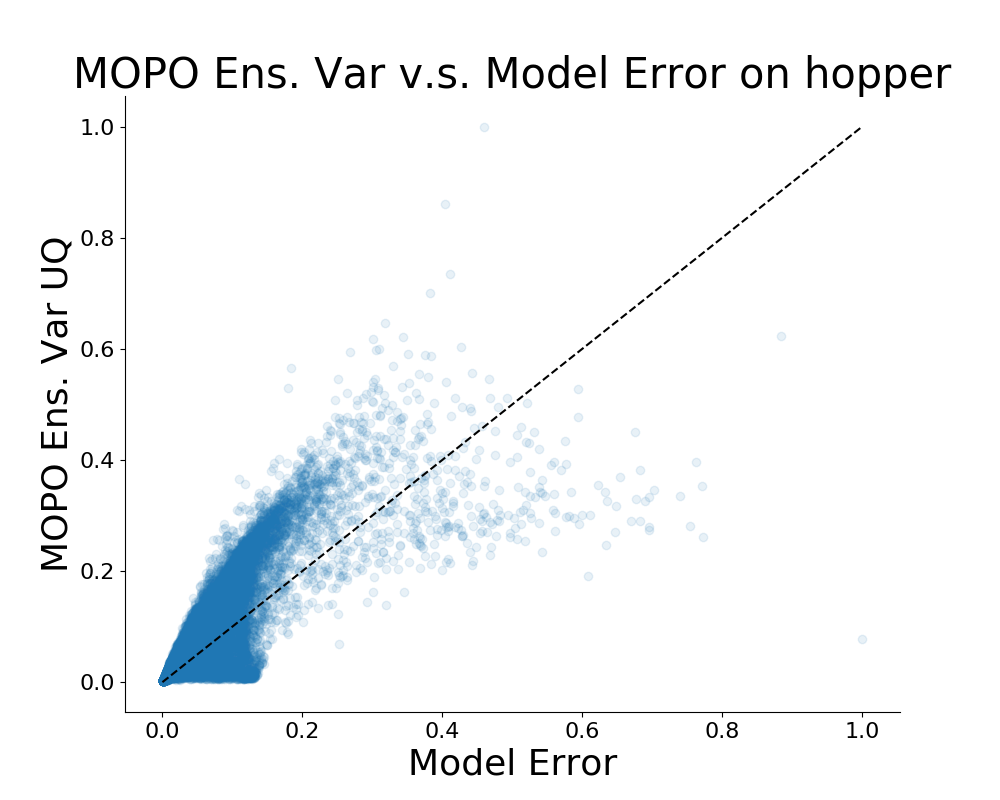
\includegraphics[width=0.47\linewidth]{hopper_medium_corr_lip_ens_ood.png}
        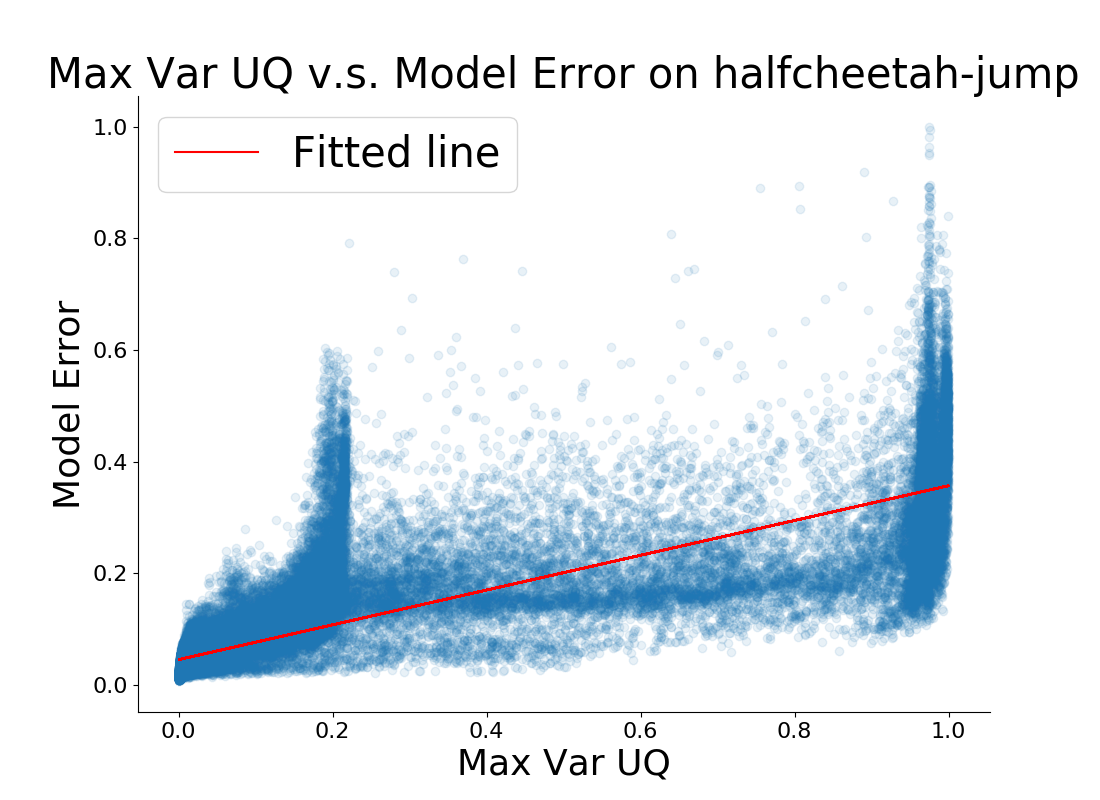
\includegraphics[width=0.45\textwidth]{chapters/combo/halfcheetah_jump_linear_regression_lip_ens_ood.png}
        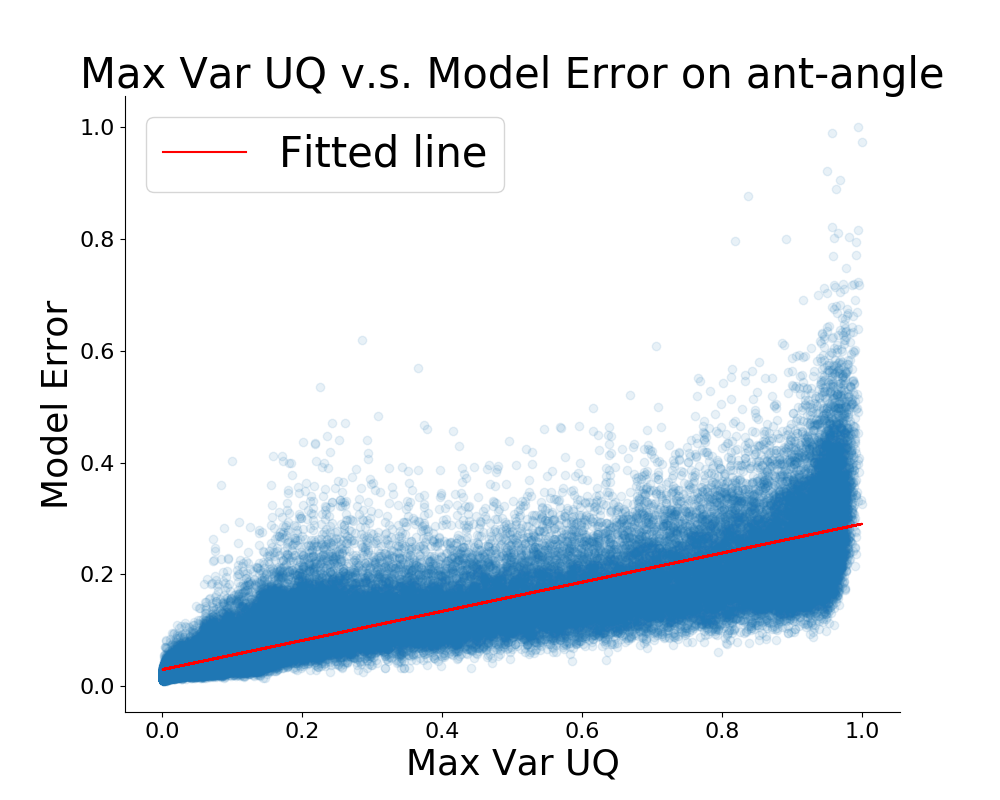
\includegraphics[width=0.41\textwidth]{chapters/combo/ant_angle_linear_regression_lip_ens_ood.png}
        \vspace{-0.2cm}
        \caption{\footnotesize {We visualize the fitted linear regression line between the model error and two uncertainty quantification methods maximum learned variance over the ensemble (denoted as \textbf{Max Var}) on two tasks that test the generalization abilities of offline RL algorithms (\texttt{halfcheetah-jump} and \texttt{ant-angle}). We show that \textbf{Max Var} struggles to predict the true model error. Such visualizations indicates that uncertainty quantification is challenging with deep neural networks and could lead to poor performance in model-based offline RL in settings where out-of-distribution generalization is needed. In the meantime, COMBO addresses this issue by removing the burden of performing uncertainty quantification.}}
        \label{fig:uq}
        \vspace{-0.4cm}
\end{figure}

In this section, we first analyze the efficacy of uncertainty estimation in existing model-based offline RL approaches. Specifically, we perform empirical evaluations to study whether uncertainty quantification with deep neural networks, especially in the setting of dynamics model learning, is challenging and could cause problems with uncertainty-based model-based offline RL methods such as MOReL~\citep{kidambi2020morel} and MOPO~\citep{yu2020mopo}. We pick tasks where the underlying model-based offline RL method is required to produce policies that need to go further away from the data distribution to obtain good performance. In our evaluations, we consider maximum learned variance over the ensemble (denoted as \textbf{Max Var}) $\max_{i=1,\dots,N}\|\Sigma^i_\theta(\bs, \mathbf{a})\|_\text{F}$ (used in MOPO).

We consider two tasks \texttt{halfcheetah-jump} and \texttt{ant-angle} (more details about the task in Appendix ??). We normalize both the model prediction error and the uncertainty estimates to be within scale $[0, 1]$ and performs linear regression that learns the mapping between the uncertainty estimates and the true model error. As shown in Figure~\ref{fig:uq}, on both tasks, \textbf{Max Var} is unable to accurately predict the true model error, suggesting that uncertainty estimation used by offline model-based methods is not accurate and might be the major factor that results in its poor performance. On the other hand, our approach, COMBO, alleviates the need for accurate uncertainty quantification by viewing model-based offline RL from the lens of conservative value function learning.

\subsection{Conservative Offline Model-Based Policy Optimization}
\label{sec:combo}
 
Our goal in this section is to develop a model-based offline RL algorithm that enables optimizing a lower bound on the policy performance, but without requiring uncertainty quantification. We achieve this by extending conservative Q-learning, from the previous section, into the model-based setting. Our algorithm, summarized in Algorithm~\ref{alg:combo}, alternates between a conservative policy evaluation step and a policy improvement step, which we outline below.

{\bf Conservative Policy Evaluation:} Given a policy $\policy$, an offline dataset $\data$, and a learned model of the MDP $\mhat$, the goal in this step is to obtain a conservative estimate of $Q^\policy$. To achieve this, we penalize the Q-values evaluated on data drawn from a particular state-action distribution that is more likely to be out-of-support while pushing up the Q-values on state-action pairs that are trustworthy, which is implemented by repeating the following recursion:

\begin{small}
\begin{align}
    \min_{Q} \beta\left(\E_{\bs, \mathbf{a} \sim \rho(\bs,\mathbf{a})}\!\left[Q(\bs,\mathbf{a})\right]-\E_{\bs, \mathbf{a} \sim \data}\left[Q(\bs,\mathbf{a})\right]\right) + \frac{1}{2}\E_{\bs, \mathbf{a}, \bs' \sim d_f}\left[ \left(Q(\bs, \mathbf{a}) - \widehat{\bellman}^\policy\hat{Q}^k(\bs, \mathbf{a}))\right)^2 \right].
    \label{eq:implicit_update}
\end{align}
\end{small}

Here, $\rho(\bs, \mathbf{a})$ and $d_f$ are sampling distributions that we can choose. Model-based algorithms allow ample flexibility for these choices while providing the ability to control the bias introduced by these choices. For $\rho(\bs, \mathbf{a})$, we make the following choice:
\[
\rho(\bs, \mathbf{a}) =  d^\policy_{\mdphat} (\bs) \pi(\mathbf{a} | \bs),
\]
where $d^\policy_{\mdphat} (\bs)$ is the discounted marginal state distribution when executing $\policy$ in the learned model $\mdphat$. Samples from $d^\policy_{\mdphat} (\bs)$ can be obtained by rolling out $\policy$ in $\mdphat$.
Similarly, $d_f$ is an $f-$interpolation between the offline dataset and rollouts from the model:
\[
d_f^\mu (\bs, \mathbf{a}) := f \ d(\bs, \mathbf{a}) + (1-f) \ d^\mu_{\mdphat} (\bs, \mathbf{a}),
\]
where $f \in [0,1]$ is the ratio of the datapoints drawn from the offline dataset as defined in Section~\ref{sec:prelim_offline_mbrl} and $\mu(\cdot | \bs)$ is the rollout distribution used with the model, which can be modeled as $\policy$ or a uniform distribution. To avoid notation clutter, we also denote $d_f := d_f^\mu$.

Under such choices of $\rho$ and $d_f$, we push down Q-values on state-action tuples from model rollouts and push up Q-values on the real state-action pairs from the offline dataset. When updating Q-values with the Bellman backup, we use a mixture of both the model-generated data and the real data, similar to Dyna~\cite{sutton1991dyna}. 
Note that in comparison to CQL and other model-free algorithms, COMBO learns the Q-function over a richer set of states beyond the states in the offline dataset. 
This is made possible by performing rollouts under the learned dynamics model, denoted by $d^\mu_{\mdphat} (\bs, \mathbf{a})$.
We will show in Section~\ref{sec:theory} that the Q function learned by repeating the recursion in Equation~\ref{eq:implicit_update} provides a lower bound on the true Q function, without the need for explicit uncertainty estimation. Furthermore, we will theoretically study the advantages of using synthetic data from the learned model, and characterize the impacts of model bias.

\begin{algorithm}[t!]
\begin{small}
  \caption{COMBO: Conservative Model Based Offline Policy Optimization}\label{alg:combo}
  \begin{algorithmic}[1]
    \Require Offline dataset $\data$, rollout distribution $\mu(\cdot|\bs)$, learned dynamics model $\widehat{T}_\theta$, initialized policy and critic  $\policy_\phi$ and $Q_\psi$.
    \State Train the probabilistic dynamics model $\widehat{T}_\theta(\bs', r|\bs,\mathbf{a}) = \mathcal{N}(\mu_\theta(\bs, \mathbf{a}), \Sigma_\theta(\bs, \mathbf{a}))$ on $\data$.
    \State Initialize the replay buffer $\data_{\text{model}} \leftarrow \varnothing$.
    \For{$i=1, 2, 3, \cdots,$}
    \State Perform rollouts by drawing samples from $\mu$ and $\widehat{T}_\theta$ starting from states in $\data$. Add model rollouts to $\data_\text{model}$.
    \State Conservatively evaluate the policy by solving eq.~\ref{eq:implicit_update} to obtain $\hat{Q}^{\policy_\phi^i}_\psi$ using data sampled from $\data \cup \data_\text{model}$.
    \State Improve policy under state marginal of $d_f$ by solving eq.~\ref{eq:combo_policy_improvement} to obtain $\policy_\phi^{i+1}$.
    \EndFor
  \end{algorithmic}
\end{small}
\end{algorithm}

{\bf Policy Improvement Using a Conservative Critic:} After learning a conservative critic $\hat{Q}^\policy$, we improve the policy as:
\begin{equation}
\label{eq:combo_policy_improvement}
\policy' \leftarrow \arg \max_{\policy} \ \mathbb{E}_{\bs \sim \rho, \mathbf{a} \sim \policy(\cdot|\bs)} \left[ \hat{Q}^{\policy} (\bs, \mathbf{a}) \right]
\end{equation}
where $\rho(\bs)$ is the state marginal of $\rho(\bs,\mathbf{a})$. When policies are parameterized with neural networks, we approximate the $\arg \max$ with a few steps of gradient descent. In addition, entropy regularization can also be used to prevent the policy from becoming degenerate if required~\cite{haarnoja2018soft}. In Section~\ref{sec:policy_improvement_theory}, we show that the resulting policy is guaranteed to improve over the behavior policy.

\textbf{Practical Implementation Details.} Our practical implementation largely follows MOPO, with the key exception that we perform conservative policy evaluation as outlined in this section, rather than using uncertainty-based reward penalties. Following MOPO, we represent the probabilistic dynamics model using a neural network, with parameters $\theta$, that produces a Gaussian distribution over the next state and reward: $\widehat{T}_\theta(\bs_{t+1}, r| \bs, \mathbf{a}) = \mathcal{N}(\mu_\theta(\bs_t, \mathbf{a}_t), \Sigma_\theta(\bs_t, \mathbf{a}_t))$. The model is trained via maximum likelihood. For training the conservative critic, which is the major distinction between COMBO and MOPO, the fixed constant $\beta$ is tuned with an offline cross-validation scheme for all low-dimensional continuous control tasks and is decided with a limited number of rollouts in the actual environment in the vision-based environments. We set the ratio $f = 0.5$ to have an equal split between model rollouts and data from the offline dataset. For conservative policy evaluation (eq.~\ref{eq:implicit_update}) and policy improvement (eq.~\ref{eq:combo_policy_improvement}), we augment $\rho$ with states sampled from the offline dataset, which shows more stable improvement in practice. Additional details about practical implementation are provided in Appendix~\ref{app:combo_details}.


\subsection{Theoretical Analysis of COMBO}
\label{sec:theory}
In this section, we theoretically analyze COMBO and show that, like CQL, it continues to optimize a lower-bound on the expected return of the learned policy. This lower bound is close to the actual policy performance (modulo sampling error) when the policy's state-action marginal distribution is in support of the state-action marginal of the behavior policy and conservatively estimates the performance of a policy otherwise. By optimizing the policy against this lower bound, COMBO guarantees policy improvement beyond the behavior policy. {Furthermore, we use these insights to discuss cases when COMBO is less conservative compared to model-free CQL}.

\begin{subsubsection}{COMBO Optimizes a Lower Bound}
\label{sec:combo_lower_bound}
We first show that training the Q-function using Equation~\ref{eq:implicit_update} produces a Q-function such that the expected off-policy policy improvement objective~\citep{degris2012off} 
%%AK.1.30: define this in the section on prelims, rather than the expected return, the expected policy improvement objective is E_{s, a \sim d_f}[Q(s, a)], which we optimize in practice and cite a number of papers (silver2014dpg, lillicrap2015ddpg, degris2021offpac).
computed using this learned Q-function lower-bounds its actual value. We will reuse notation for $d_f$ and $d$ from Sections~\ref{sec:prelim} and~\ref{sec:combo}. 
% With a slight abuse of notation, we will assume that $d_f$ and $\data$ denote (empirical) distributions over the state-action space.
%%TY.1.31: it's a bit unclear what D_f is. In Section 4, it is currently defined as the interpolation, but here it seems to refer to an arbitrary state-action distribution.
Assuming that the Q-function is tabular, the Q-function found by approximate dynamic programming in iteration $k$, can be obtained by differentiating Equation~\ref{eq:implicit_update} with respect to $Q^k$ (see App.~\ref{app:proofs} for details):
\begin{equation}
    \hat{Q}^{k+1}(\bs, \mathbf{a}) = (\widehat{\mathcal{B}}^\pi Q^k)(\bs, \mathbf{a}) - \beta \frac{\rho(\bs, \mathbf{a}) - d(\bs, \mathbf{a})}{d_f(\bs, \mathbf{a})}.
\label{eqn:combo_iterate}
\end{equation}
Equation~\ref{eqn:combo_iterate} effectively applies a penalty that depends on the three distributions appearing in the COMBO critic training objective (Equation~\ref{eq:implicit_update}), of which $\rho$ and $d_f$ are free variables that we choose in practice as discussed in Section~\ref{sec:combo}. For a given iteration $k$ of Equation~\ref{eqn:combo_iterate}, we further define the expected penalty under $\rho(\bs, \mathbf{a})$ as: 
\begin{equation}
 \nu(\rho, f) := \E_{\bs, \mathbf{a} \sim \rho(\bs, \mathbf{a})}\left[\frac{\rho(\bs, \mathbf{a}) - d(\bs, \mathbf{a})}{d_f(\bs, \mathbf{a})} \right]\label{eqn:expected_penalty}.
\end{equation}
% Before stating our main result, we will first show that the penalty term in Equation~\ref{eqn:combo_iterate} is positive in expectation. Such a positive penalty is important to combat any overestimation that may arise as a result of using $\bellmanhat$. 

% \begin{lemma}[Interpolation Lemma]
% \label{thm:line_thm}
% For any $f \in [0, 1]$, and any given $\rho(\bs, \mathbf{a}) \in \Delta^{|\states||\actions|}$, let $d_f$ be an f-interpolation of $\rho$ and $\data$, i.e., $d_f(\bs, \mathbf{a}) := f d(\bs, \mathbf{a}) + (1-f) \rho(\bs, \mathbf{a})$. For a given iteration $k$ of Equation~\ref{eqn:combo_iterate}, define the expected penalty under $\rho(\bs, \mathbf{a})$ as: 
% \begin{equation*}
%  \nu(\rho, f) := \E_{\rho}\left[\frac{\rho(\bs, \mathbf{a}) - d(\bs, \mathbf{a})}{d_f(\bs, \mathbf{a})} \right].
% \end{equation*}
% Then $\nu(\rho, f)$ satisfies, (1) $\nu(\rho, f) \geq 0,~~ \forall \rho, f$, (2) $\nu(\rho, f)$ is monotonically increasing in $f$ for a fixed $\rho$, and (3) $\nu(\rho, f) = 0$ iff $\forall~ \bs, \mathbf{a}, ~\rho(\bs, \mathbf{a}) = d(\bs, \mathbf{a}) \text{~or~} f = 0$. 
% \end{lemma}
% The proof can be found in Appendix~\ref{app:proof_lemma}.
% Lemma~\ref{thm:line_thm} characterizes $\rho(\bs, \mathbf{a})$ for which COMBO (Equation~\ref{eq:implicit_update}) induces a conservative penalty. 
% COMBO sets $\rho(\bs) = d^\pi_{\mdphat}(\bs)$ 
% %%SL.1.31: Nitpick: you defined D_f(s,a) before, not D_f(s). While it's easy to guess what D_f(s) is, it is undefined
% and uses $\rho(\mathbf{a}|\bs) = \pi(\mathbf{a}|\bs)$, and hence each step of update (Equation~\ref{eqn:combo_iterate}) penalizes the Q-function making it more conservative. The total amount of conservatism induced in the Q-function, given by $\nu(\rho, f)$, is controlled by the choice of $f$. Based on result (2) in Lemma~\ref{thm:line_thm}, we note that by controlling the amount of real data, $f$, we can control the amount of conservatism: $f=1$ induces the maximum conservatism, and $f=0$ induces no conservatism at all.

% Next, we will show that the asymptotic Q-function learned by COMBO lower-bounds the actual Q-function of any policy $\pi$ with high probability for a large enough $\beta \geq 0$. Let $\mdpbar$ represent the empirical MDP which uses the empirical transition model based on raw data counts. The Bellman backups over the dataset distribution $d_f$ in equation~\ref{eq:implicit_update} can be interpreted as an $f-$interpolation 
% of the backup operator in the empirical MDP (denoted by $\bellman_{\mdpbar}^\pi$) and the backup operator under the learned model $\mdphat$ (denoted by $\bellman_{\mdphat}^\pi$).
% The empirical backup operator suffers from sampling error, but is unbiased in expectation, whereas the model backup operator induces bias but no sampling error.
% We assume that all of these backups enjoy concentration properties with concentration coefficient $C_{r, T, \delta}$, dependent on the desired confidence value $\delta$ (details in Appendix~\ref{app:proof_lower_bound}). This is a standard assumption in literature~\citep{laroche2019safe}.
% Now, we state our main results below.

% \begin{proposition}[Asymptotic lower-bound]
% \label{thm:Q_bound}
% Let $P^\pi$ denote the Hadamard product of the dynamics $P$ and a given policy $\pi$ in the actual MDP and let $S^\pi := (I - \gamma P^\pi)^{-1} c_{S}$, where $c_{S}$ is a suitably chosen positive constant. Let $D$ denote the total-variation divergence between two probability distributions. For any $\pi(\mathbf{a}|\bs)$, the Q-function obtained by recursively applying Equation~\ref{eqn:combo_iterate}, with $\hat{{\bellman}}^\pi = f \bellman_{\mdpbar}^\pi + (1 - f) \bellman_{\mdphat}^\pi$, with probability at least $1 - \delta$, results in $\hat{Q}^\pi$ that satisfies:
% \begin{align*}
%     \forall \bs, \mathbf{a},~ \hat{Q}^\pi(\bs, \mathbf{a}) \leq  Q^\pi(\bs, \mathbf{a}) - \beta \cdot \epsilon_{\text{c}} + f \epsilon_{\text{s}} + (1 - f)\epsilon_{\text{m}},
% \end{align*}
% where vector forms of $\epsilon_{\text{s}}$, $\epsilon_{\text{c}}$ and $\epsilon_{\text{m}}$ are given by:
% %%CF: Is there a reason why you chose this order? It would be more intuititve for me to have the order match the order that they appear in the inequality above.
% \small{
% \begin{align*}
%     \epsilon_{\text{c}} := \left[ \frac{1}{c_S} S^\pi \left[ \frac{\rho - d}{d_f} \right] \right], \epsilon_{\text{m}} := \left[ S^\pi \left[ |R - R_{\mdphat}| \!+\! \frac{ 2 \gamma  R_{\max}}{1 - \gamma} D(P, P_{\mdphat}) \right]  \right],~ \epsilon_{\text{s}} &:= \left[ S^\pi \left[ \frac{C_{r, T, \delta} R_{\max}}{(1 - \gamma) \sqrt{|\data|}} \right] \right].
%     %%CF: Has the distance D been defined?
% \end{align*}
% }
% \end{proposition}
% The proof for Proposition~\ref{thm:Q_bound} can be found in Appendix~\ref{app:proof_lower_bound}. 

Next, we will show that the Q-function learned by COMBO lower-bounds the actual Q-function under the initial state distribution $\mu_0$ and any policy $\pi$. We also show that the asymptotic Q-function learned by COMBO lower-bounds the actual Q-function of any policy $\pi$ with high probability for a large enough $\beta \geq 0$, which we include in Appendix~\ref{app:proof_lower_bound}. Let $\mdpbar$ represent the empirical MDP which uses the empirical transition model based on raw data counts. The Bellman backups over the dataset distribution $d_f$ in equation~\ref{eq:implicit_update} can be interpreted as an $f-$interpolation 
of the backup operator in the empirical MDP (denoted by $\bellman_{\mdpbar}^\pi$) and the backup operator under the learned model $\mdphat$ (denoted by $\bellman_{\mdphat}^\pi$).
The empirical backup operator suffers from sampling error, but is unbiased in expectation, whereas the model backup operator induces bias but no sampling error.
We assume that all of these backups enjoy concentration properties with concentration coefficient $C_{r, T, \delta}$, dependent on the desired confidence value $\delta$ (details in Appendix~\ref{app:proof_lower_bound}). This is a standard assumption in literature~\citep{laroche2019safe}.
Now, we state our main results below.
\begin{theorem}
\label{thm:lower_bound}
For large enough $\beta$, we have
$\E_{\bs \sim \mu_0, \mathbf{a} \sim \policy(\cdot|\bs)}[\hat{Q}^\pi(\bs, \mathbf{a})] \leq \E_{\bs \sim \mu_0, \mathbf{a} \sim \policy(\cdot|\bs)}[Q^\pi(\bs, \mathbf{a})]$, 
where $\mu_0(\bs)$ is the initial state distribution. 
Furthermore, when $\epsilon_{\text{s}}$ is small, such as in the large sample regime, or when the model bias $\epsilon_{\text{m}}$ is small, a small $\beta$ is sufficient to guarantee this condition along with an appropriate choice of $f$.
\end{theorem}
%%SL.5.24: Could we explain a bit more intuitively what the significance of a small beta being sufficient is?

The proof for Proposition~\ref{thm:lower_bound} can be found in Appendix~\ref{app:proof_lower_bound}.
% Corollary~\ref{thm:lower_bound} directly appeals to Proposition~\ref{thm:Q_bound} and Lemma~\ref{thm:line_thm}.
% Proposition~\ref{thm:Q_bound} further implies that for large $\beta$,
%%CF: I think you mean "for large beta" or "for non-zero beta" here?
% deviating away from the behavior policy is expected to lead to smaller values.
Finally, while \citet{kumar2020conservative} also analyze how regularized value function training can provide lower bounds on the value function at each state in the dataset~\citep{kumar2020conservative} (Proposition 3.1-3.2), \textit{our result shows that COMBO is less conservative in that it does not underestimate the value function at every state in the dataset like CQL (Remark~\ref{remak:tighter_lower_bound})} and might even overestimate these values. Instead COMBO penalizes Q-values at states generated via model rollouts from $\rho(\bs, \mathbf{a})$. While it is challenging to argue that that either COMBO or CQL attains the tightest possible lower-bound on return, in our final result of this section, we discuss a sufficient condition for the COMBO lower-bound to be tighter than CQL. 

\begin{tcolorbox}[colback=blue!6!white,colframe=black,boxsep=0pt,top=3pt,bottom=5pt]
\begin{theorem}[CQL vs COMBO]
%%CF.5.25: can we give a name to this? (like was done for 4.1)
\label{prop:less_conservative}
Let $\Delta^\pi_{\text{COMBO}} := \E_{\bs, \mathbf{a} \sim d_{\mdpbar}(\bs), \pi(\mathbf{a}|\bs)}\left[ \hat{Q}^\pi(\bs, \mathbf{a}) \right]$ and $\Delta^\pi_{\text{CQL}} := \E_{\bs, \mathbf{a} \sim d_{\mdpbar}(\bs), \pi(\mathbf{a}|\bs)}\left[ \hat{Q}^\pi_\text{CQL}(\bs, \mathbf{a}) \right]$ denote the average values on the dataset under the Q-functions learned by COMBO and CQL respectively. 
%%CF.5.25: put notation outside of the Proposition statement?
Then, $\Delta^\pi_{\text{COMBO}} \geq \Delta^\pi_\text{CQL}$, if:
\begin{equation*}
    \E_{\bs, \mathbf{a} \sim \rho(\bs,\mathbf{a})}\left[ \frac{\pi(\mathbf{a}|\bs)}{\behavior(\mathbf{a}|\bs)} \right] - \E_{\bs, \mathbf{a} \sim d_{\mdpbar}(\bs), \pi(\mathbf{a}|\bs)}\left[ \frac{\pi(\mathbf{a}|\bs)}{\behavior(\mathbf{a}|\bs)} \right] \leq 0.~~~~~~~~~~~(*)
    % \sum_{\bs, \mathbf{a}} \left(\rho(\bs) - d_{\mdpbar}(\bs)\right) \frac{\pi^2(\mathbf{a}|\bs)}{\behavior(\mathbf{a}|\bs)} \leq 0.~~~~~~~~~~~(*)
\end{equation*}
\end{theorem}
\end{tcolorbox}
Proposition~\ref{prop:less_conservative} indicates that COMBO will be less conservative than CQL when the action probabilities under learned policy $\pi(\mathbf{a}|\bs)$ and the probabilities under the behavior policy $\pi_\beta(\mathbf{a}|\bs)$ are closer together on state-action tuples drawn from $\rho(\bs, \mathbf{a})$ (i.e., sampled from the model using the policy $\pi(\mathbf{a}|\bs)$), than they are on states from the dataset and actions from the policy, $d_{\mdpbar}(\bs)\pi(\mathbf{a}|\bs)$.
%%SL.5.24: The above sentences are easy to misunderstand. Can we rephrase like this: when the action probabilities under learned policy $\pi(\mathbf{a}|\bs)$ and the probabilities under the behavior policy $\pi_\beta(\mathbf{a}|\bs)$ are closer together on state-action tuples drawn from $\rho(\bs, \mathbf{a})$ (i.e., sampled from the model using the policy $\pi(\mathbf{a}|\bs)$), than they are on states from the dataset and actions from the policy, $d_{\mdpbar}(\bs)\pi(\mathbf{a}|\bs)$. [that said, I'm not sure this intuition is quite right...]
COMBO's objective (Equation~\ref{eq:implicit_update}) only penalizes Q-values under $\rho(\bs, \mathbf{a})$, which, in practice, are expected to primarily consist of out-of-distribution states generated from model rollouts, and does not penalize the Q-value at states drawn from $d_{\mdpbar}(\bs)$. As a result, the expression $(*)$ is likely to be negative, making COMBO less conservative than CQL.
%%CF.5.25:  It would be really good to talk about what this means in combination with prop 4.1. In isolation, this result is of course not meaningful on its own. (i.e. lower-bound plus often less conservative means often closer to the actual Q-value. (unless I am misunderstanding something here)

%%SL.5.24: I'm not sure I follow this logic -- why should we expect it to be negative?
% COMBO does not underestimate the value function at every state in the dataset like \citet{kumar2020conservative}, but only lower-bounds the expected value function under the initial state distribution as discussed in Corollary~\ref{thm:lower_bound}. We elaborate on how COMBO is less conservative as it attains tighter lower bounds in Remark~\ref{remak:tighter_lower_bound} (Appendix~\ref{app:proof_lower_bound}).

\subsubsection{Model-Based Safe Policy Improvement}

\label{sec:policy_improvement_theory}
Now that we have shown various aspects of the lower-bound on the Q-function induced by COMBO, we provide policy improvement guarantees for the COMBO algorithm. Formally, Proposition~\ref{thm:policy_improvement} discuss safe improvement guarantees over the behavior policy. building on prior work~\citep{petrik2016safe,laroche2019safe,kumar2020conservative}. 

\begin{tcolorbox}[colback=blue!6!white,colframe=black,boxsep=0pt,top=3pt,bottom=5pt]
\begin{theorem}[$\zeta$-safe policy improvement]
\label{thm:policy_improvement}
Let $\hat{\pi}_{\text{out}}(\mathbf{a}|\bs)$ be the policy obtained by COMBO. Then, the policy $\hat{\pi}_{\text{out}}(\mathbf{a}|\bs)$ is a $\zeta$-safe policy improvement over ${\behavior}$ in the actual MDP $\mdp$, i.e., $J(\hat{\pi}_{\text{out}}, \mdp) \geq J({\behavior}, \mdp) - \zeta$, with probability at least $1 - \delta$, where $\zeta$ is given by,
\small{
\begin{align*}
    \mathcal{O}\left(\frac{\gamma f}{(1 - \gamma)^2}\right) ~&\underbrace{\E_{\bs \sim d^{\hat{\pi}_{\text{out}}}_{\mdp}}\left[ \sqrt{\frac{|\actions|}{|\data(\bs)|} \mathrm{D}_{\text{CQL}}(\hat{\pi}_{\text{out}}, \behavior)} \right]}_{:=~ \text{(1)}}\\
    &+ \mathcal{O}\left(\frac{\gamma (1 - f)}{(1 - \gamma)^2}\right) \underbrace{ \mathrm{D_{TV}}(\mdpbar, \mdphat)}_{:=~ \text{(2)}} - \underbrace{\beta \frac{\nu(\rho^\pi, f) - \nu(\rho^\beta, f)}{(1 - \gamma)}}_{:=~ \text{(3)}}.
\end{align*}
}
\end{theorem}
\end{tcolorbox}

The complete statement (with constants and terms that grow smaller than quadratic in the horizon) and proof for Proposition~\ref{thm:policy_improvement} is provided in Appendix~\ref{app:proof_policy_improvement}. $D_{\text{CQL}}$ denotes a notion of probabilistic distance between policies~\citep{kumar2020conservative} which we discuss further in Appendix~\ref{app:proof_policy_improvement}. The expression for $\zeta$ in Proposition~\ref{thm:policy_improvement} consists of three terms: term (1)~captures the decrease in the policy performance due to limited data, and decays as the size of $\mathcal{D}$ increases. The second term (2)~captures the suboptimality induced by the bias in the learned model. Finally, as we show in Appendix~\ref{app:proof_policy_improvement}, the third term (3)~is equivalent to the improvement in policy performance as a result of running COMBO in the empirical and model MDPs. Since the learned model is trained on the dataset $\data$ with transitions generated from the behavior policy $\behavior$, the marginal distribution $\rho^\beta(\bs, \mathbf{a})$ is expected to be closer to $d(\bs, \mathbf{a})$ for $\behavior$ as compared to the counterpart for the learned policy, $\rho^\pi$. Thus, term (3) is expected to be positive in practice, and in such cases, an appropriate (large) choice of $\beta$ will make term (3) large enough to counteract terms (1) and (2) that reduce policy performance. We discuss this elaborately in Appendix~\ref{app:proof_policy_improvement} (Remark~\ref{remark:remark1}). 

Further note that in contrast to Proposition 3.6 in \citet{kumar2020conservative}, note that our result indicates the sampling error (term (1)) is reduced (multiplied by a fraction $f$) when a near-accurate model is used to augment data for training the Q-function, \neurips{and similarity, it can avoid the bias of model-based methods by relying more on the model-free component. This allows COMBO to attain the best-of-both model-free and model-based methods, via a suitable choice of the fraction $f$.}

% \textcolor{red}{[if the above stuff makes sense -- it is just setting model error and Q-function sampling error in a way so as to optimize for a non-zero f -- I can formally write it down. However the assumption is a bit adhoc -- it is unclear why model-bias is large when sampling error ir small, but we will have to assume this.]}


To summarize, through an appropriate choice of $f$, Proposition~\ref{thm:policy_improvement} guarantees safe improvement over the behavior policy without requiring access to an oracle uncertainty estimation algorithm.
% Proposition~\ref{thm:policy_improvement} only depends on an appropriate choice single, scalar $f \in [0, 1]$, which can be controlled in practice and gets rid of the strict requirement of oracle access to a uniformly-accurate uncertainty metric.   
%%CF: Can we put this in the opposite order to match the order in the previous sentences?
\end{subsection}


\vspace{-0.2cm}
\subsection{Experimental Evaluation of COMBO}
\label{sec:combo_exp}
\vspace{-0.2cm}

In our experiments, we aim to answer the follow questions: \textbf{(1)} Can COMBO generalize better than previous offline model-free and model-based approaches in a setting that requires generalization to tasks that are different from what the behavior policy solves? \textbf{(2)} How does COMBO compare with prior work in tasks with high-dimensional image observations?, \textbf{(3)} How does COMBO compare to prior offline model-free and model-based methods in standard offline RL benchmarks?

To answer those questions, we compare COMBO to several prior methods. In the domains with compact state spaces, we compare with recent model-free algorithms like BEAR~\citep{kumar2019stabilizing}, BRAC~\citep{wu2019behavior}, and the CQL~\citep{kumar2020conservative} algorithm presented in the previous section; as well as MOPO~\citep{yu2020mopo} {and MOReL~\citep{kidambi2020morel} which are two recent model-based algorithms}. In addition, we also compare with an offline version of SAC~\citep{haarnoja2018soft} (denoted as SAC-off), and behavioral cloning (BC). In high-dimensional image-based domains, which we use to answer question (3), we compare to LOMPO~\citep{Rafailov2020LOMPO}, which is a latent space offline model-based RL method that handles image inputs, latent space MBPO (denoted LMBPO), similar to \citet{janner2019trust} which uses the model to generate additional synthetic data, the fully offline version of SLAC \citep{lee2019SLAC} (denoted SLAC-off), which only uses a variational model for state representation purposes, and CQL from image inputs. To our knowledge, CQL, MOPO, and LOMPO are representative of state-of-the-art model-free and model-based offline RL methods. Hence we choose them as comparisons to COMBO. For more details of our experimental set-up, comparisons, and hyperparameters, see Appendix~\ref{app:details}.

\vspace{-0.1cm}
\subsubsection{Results on tasks that require generalization}
\label{sec:generalization_exps}
\vspace{-0.2cm}

\begin{table}
\centering
\scriptsize
\resizebox{0.99\textwidth}{!}{\begin{tabular}{l|r|r|r|r|r|r}
\toprule 
\textbf{Environment} & \stackanchor{\textbf{Batch}}{\textbf{Mean}} & \stackanchor{\textbf{Batch}}{\textbf{Max}} & \stackanchor{\textbf{COMBO}} {\textbf{(Ours)}} & \textbf{MOPO} & {\textbf{MOReL}} & \textbf{CQL}\\ \midrule
halfcheetah-jump & -1022.6 & 1808.6 & \textbf{5392.7} & 4016.6 & {3228.7} & 741.1\\
ant-angle & 866.7 & 2311.9 & \textbf{2764.8} & 2530.9 & {2660.3} & 2473.4\\
sawyer-door-close & 5\% & 100\% & \textbf{100}\% & 65.8\% & 42.9\% & 36.7\%\\
\bottomrule
\end{tabular}}
\vspace{-0.2cm}
\caption{
\footnotesize Average returns of \texttt{halfcheetah-jump} and \texttt{ant-angle} and average success rate of \texttt{sawyer-door-close} that require out-of-distribution generalization. All results are averaged over 3 random seeds. We include the mean and max undiscounted return / success rate of the episodes in the batch data (under Batch Mean and Batch Max, respectively) for comparison.
}
\vspace{-0.3cm}
\label{tbl:generalize}
\normalsize
\end{table}

To answer question (1), we use the two environments \texttt{halfcheetah-jump} and \texttt{ant-angle} constructed in \citet{yu2020mopo}, which requires the agent to solve a task that is different from what the behavior policy solved. In both environments, the offline dataset is collected by policies trained with the original reward functions of \texttt{halfcheetah} and \texttt{ant}, which reward the halfcheetah and the ant to run as fast as possible. The behavior policies are trained with SAC with 1M steps and we take the full replay buffer as the offline dataset. Following \citet{yu2020mopo}, we relabel the rewards in the offline datasets to reward the halfcheetah to jump as high as possible and the ant to run to the top corner with a 30 degree angle as fast as possible. Following the same manner, we construct a third task \texttt{sawyer-door-close} based on the environment in \citet{yu2020meta, Rafailov2020LOMPO}. In this task, we collect the offline data with SAC policies trained with a sparse reward function that only gives a reward of 1 when the door is \textit{opened} by the sawyer robot and 0 otherwise. The offline dataset is similar to the ``medium-expert`` dataset in the D4RL benchmark since we mix equal amounts of data collected by a fully-trained SAC policy and a partially-trained SAC policy. We relabel the reward such that it is 1 when the door is \textit{closed} and 0 otherwise. Therefore, in these datasets, the offline RL methods must generalize beyond behaviors in the offline data in order to learn the intended behaviors. We visualize \texttt{sawyer-door-close} on the right in Figure~\ref{fig:visual} in Appendix~\ref{app:image_details}.

We present the results on the three tasks in Table~\ref{tbl:generalize}. {COMBO significantly outperforms MOPO, MOReL and CQL, two representative model-based methods and one representative model-free methods respectively}, in the \texttt{halfcheetah-jump} and \texttt{sawyer-door-close} tasks, and {achieves an approximately 8\%, 4\% and 12\% improvement over MOPO, MOReL and CQL respectively on the \texttt{ant-angle} task}. {These results validate that COMBO achieves better generalization results in practice by behaving less conservatively than prior model-free offline methods (compare to CQL, which doesn't improve much) and more robustly than prior model-based offline methods (compare to MOReL and MOPO).}

% \subsubsection{Empirical analysis on uncertainty estimation in offline model-based RL}
% \label{sec:uq}

% \begin{figure}
%     \vspace{-0.5cm}
%         \centering
%         % 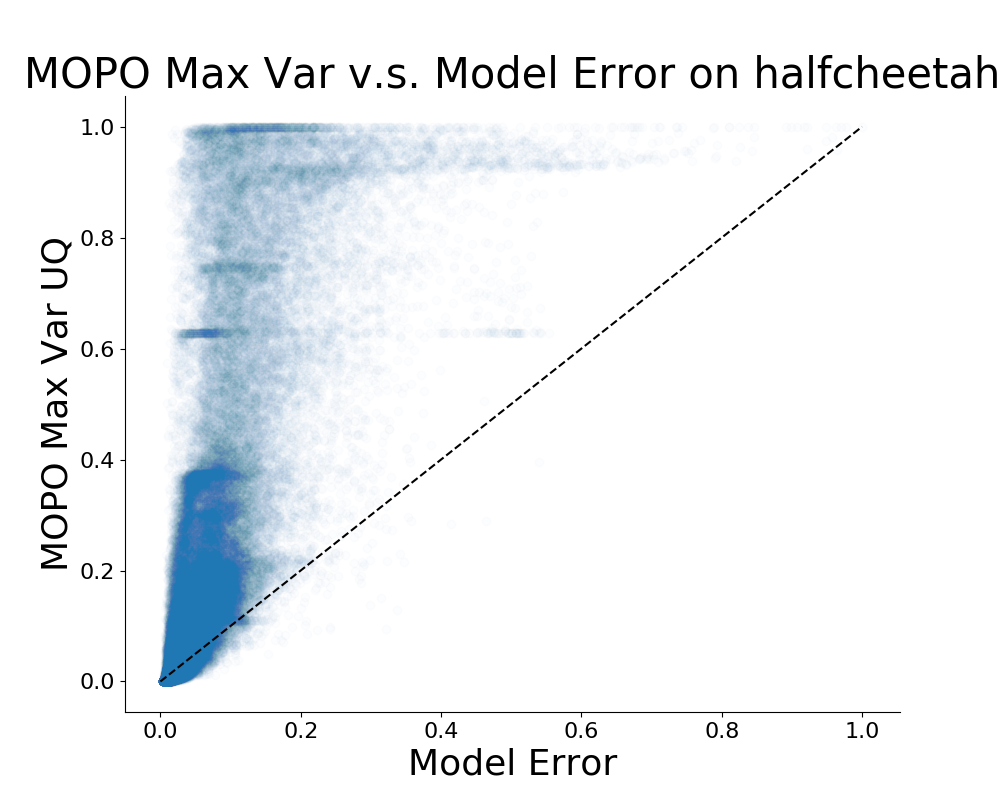
\includegraphics[width=0.47\linewidth]{halfcheetah_medium_corr_var_ood.png}
%         % 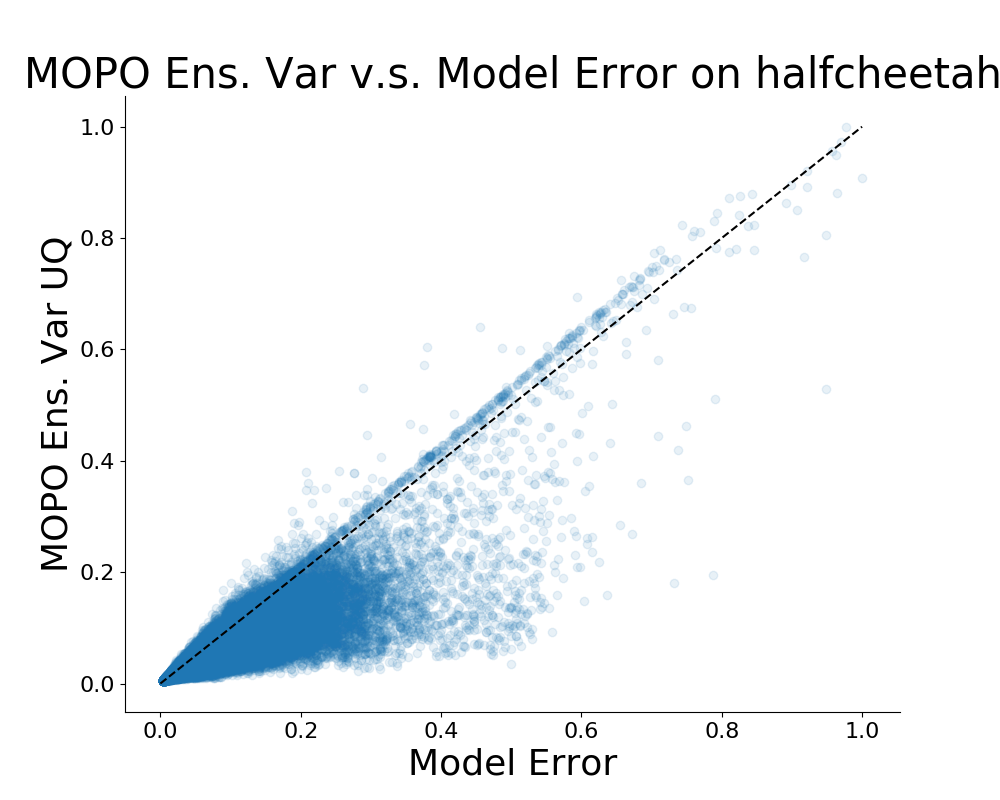
\includegraphics[width=0.47\linewidth]{halfcheetah_medium_corr_lip_ens_ood.png}
%         % 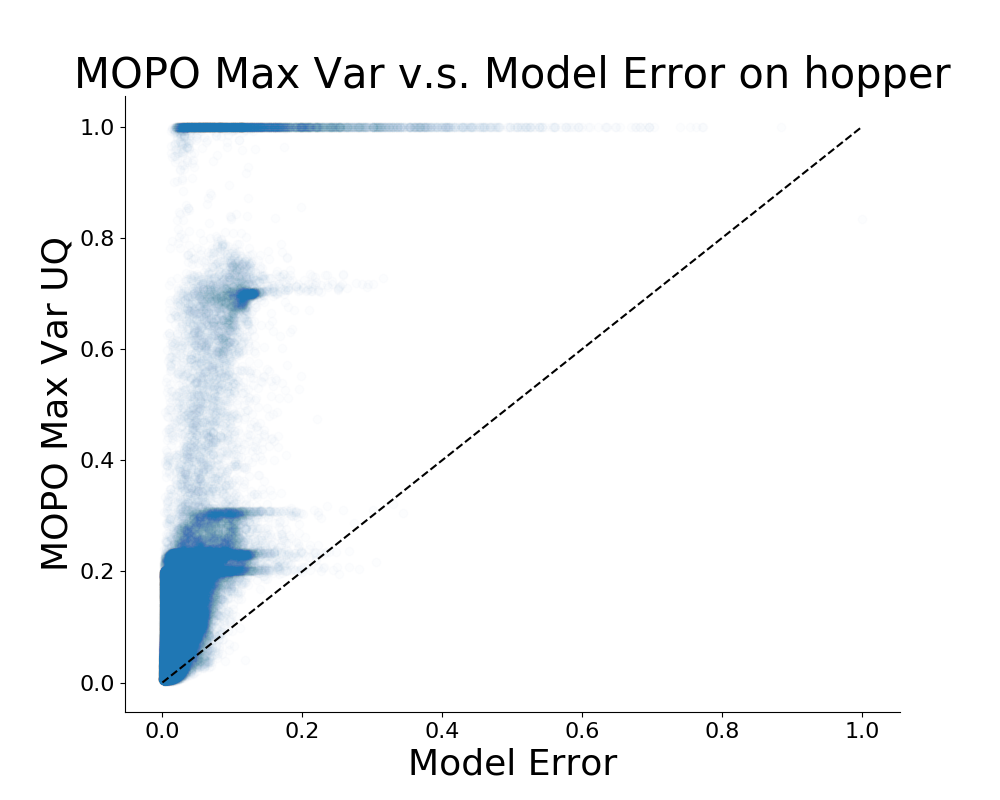
\includegraphics[width=0.47\linewidth]{hopper_medium_corr_var_ood.png}
%         % 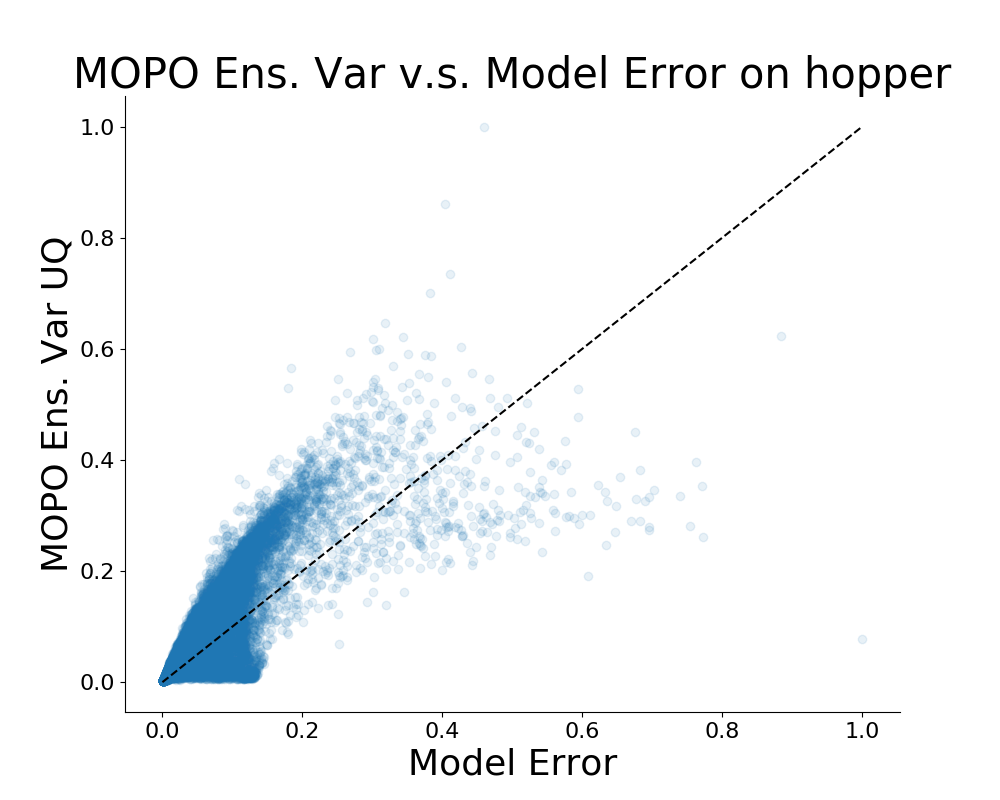
\includegraphics[width=0.47\linewidth]{hopper_medium_corr_lip_ens_ood.png}
%         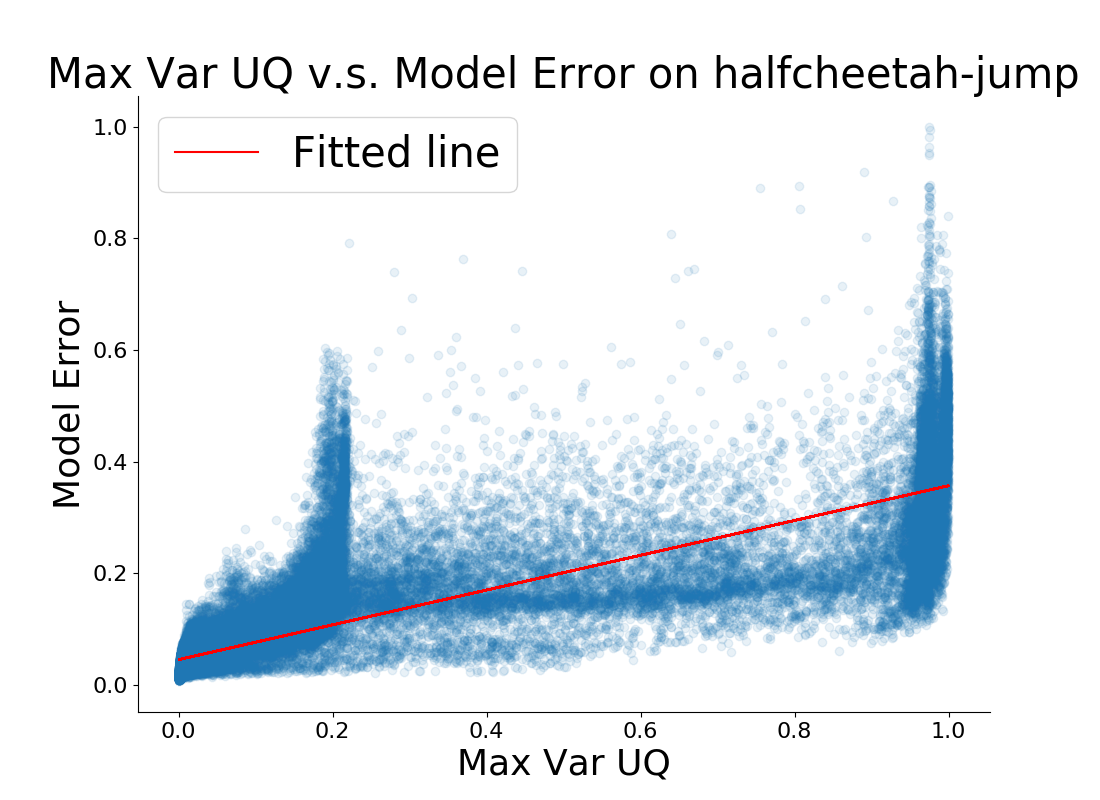
\includegraphics[width=0.45\textwidth]{chapters/combo/halfcheetah_jump_linear_regression_lip_ens_ood.png}
%         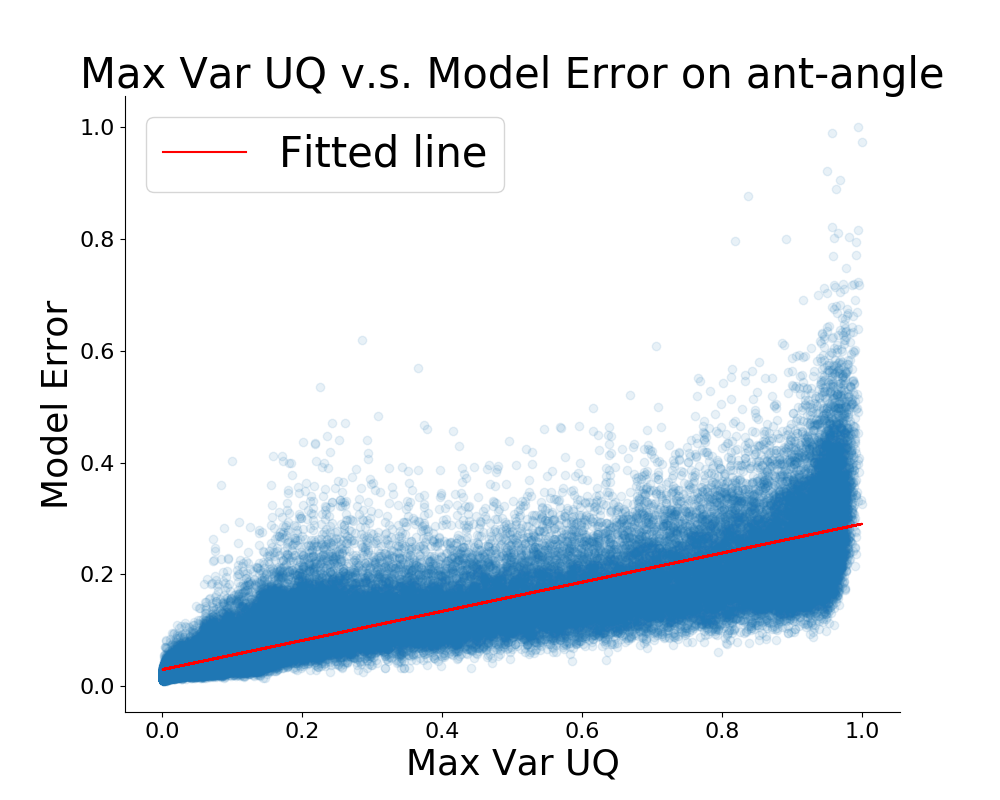
\includegraphics[width=0.41\textwidth]{chapters/combo/ant_angle_linear_regression_lip_ens_ood.png}
%         \vspace{-0.2cm}
%         \caption{\footnotesize {We visualize the fitted linear regression line between the model error and two uncertainty quantification methods maximum learned variance over the ensemble (denoted as \textbf{Max Var}) on two tasks that test the generalization abilities of offline RL algorithms (\texttt{halfcheetah-jump} and \texttt{ant-angle}). We show that \textbf{Max Var} struggles to predict the true model error. Such visualizations indicates that uncertainty quantification is challenging with deep neural networks and could lead to poor performance in model-based offline RL in settings where out-of-distribution generalization is needed. In the meantime, COMBO addresses this issue by removing the burden of performing uncertainty quantification.}}
%         \label{fig:uq}
%         \vspace{-0.4cm}
% \end{figure}

% {To further understand why COMBO outperforms prior model-based methods in tasks that require generalization, we argue that one of the main reasons could be that uncertainty estimation is hard in these tasks where the agent is required to go further away from the data distribution. To test this intuition, we perform empirical evaluations to study whether uncertainty quantification with deep neural networks, especially in the setting of dynamics model learning, is challenging and could cause problems with uncertainty-based model-based offline RL methods such as MOReL~\citep{kidambi2020morel} and MOPO~\citep{yu2020mopo}. In our evaluations, we consider maximum learned variance over the ensemble (denoted as \textbf{Max Var}) $\max_{i=1,\dots,N}\|\Sigma^i_\theta(\bs, \mathbf{a})\|_\text{F}$ (used in MOPO).

% We consider two tasks \texttt{halfcheetah-jump} and \texttt{ant-angle}. We normalize both the model error and the uncertainty estimates to be within scale $[0, 1]$ and performs linear regression that learns the mapping between the uncertainty estimates and the true model error. As shown in Figure~\ref{fig:uq}, on both tasks, \textbf{Max Var} is unable to accurately predict the true model error, suggesting that uncertainty estimation used by offline model-based methods is not accurate and might be the major factor that results in its poor performance. Meanwhile, COMBO circumvents challenging uncertainty quantification problem and achieves better performances on those tasks, indicating the effectiveness of the method.}

\vspace{-0.2cm}
\subsubsection{Results on Image-Based Tasks}
\vspace{-0.2cm}
To answer question (2), we evaluate COMBO on two image-based tasks: the standard walker (\texttt{walker-walk}) task from the the DM Control suite \cite{tassa2018deepmind} and a visual door opening environment with a Sawyer robotic arm (\texttt{sawyer-door}) as used in Section~\ref{sec:generalization_exps}. For the walker task we construct 4 datasets: medium-replay (M-R), medium (M), medium-expert (M-E), and expert, similar to \citet{fu2020d4rl}, each consisting of 200 trajectories. For \texttt{sawyer-door} task we use only the medium-expert and the expert datasets, due to the sparse reward -- the agent is rewarded only when it successfully opens the door. Both environments are visulized in Figure~\ref{fig:visual} in Appendix~\ref{app:image_details}. To extend COMBO to the image-based setting, we follow \citet{Rafailov2020LOMPO} and train a recurrent variational model using the offline data and use train COMBO in the latent space of this model.

\begin{table}
\vspace{-0.2cm}
\centering
\scriptsize
\resizebox{0.75\textwidth}{!}{\begin{tabular}{l|l|r|r|r|r|r}
\toprule
\textbf{\!\!\!Dataset\!\!} & \textbf{Environment} & \vtop{\hbox{\bf \strut COMBO (Ours)}}  & \textbf{LOMPO}& \textbf{LMBPO}& \vtop{\hbox{\bf \strut SLAC-Off}} & \textbf{CQL}\\ \midrule
\!\!\!M-R           & walker\_walk & \textbf{69.2}  & 66.9 & 59.8  & 45.1 & 15.6          \\
\!\!\!M             & walker\_walk & 57.7  & 60.2 & \textbf{61.7}  & 41.5 & 38.9          \\
\!\!\!M-E           & walker\_walk & 76.4  & \textbf{78.9} & 47.3  & 34.9 & 36.3          \\
\!\!\!expert        & walker\_walk & \textbf{61.1}  & 55.6 & 13.2  & 12.6 & 43.3          \\
\!\!\!M-E\!\!\!     & sawyer-door &\textbf{100.0\%} & \textbf{100.0\%}& 0.0\%  & 0.0\% & 0.0\% \\
\!\!\!expert\!\!\!        & sawyer-door &\textbf{96.7\%}  & 0.0\%           & 0.0\% & 0.0\%  & 0.0\% \\
\bottomrule
\end{tabular}}
\vspace{-0.2cm}
\caption{\footnotesize Results for vision experiments. %
For the Walker task each number is the normalized score proposed in \cite{fu2020d4rl} of the policy at the last iteration of training, averaged over 3 random seeds. For the Sawyer task, we report success rates over the last 100 evaluation runs of training. For the dataset, M refers to medium, M-R refers to medium-replay, and M-E refers to medium expert.}
\label{tbl:vision}
\normalsize
\vspace{-0.5cm}
\end{table}

We present results in Table~\ref{tbl:vision}. On the \texttt{walker-walk} task, COMBO performs in line with LOMPO and previous methods. On the more challenging Sawyer task, COMBO matches LOMPO and achieves 100\% success rate on the medium-expert dataset, and substantially outperforms all other methods on the narrow expert dataset, achieving an average success rate of 96.7\%, when all other model-based and model-free methods fail. 
%%CF: Need to describe the walker results
%%RR: Added a sentence, perhaps shouldn't focus on it too much - pefromance is comparable to LOMPO?


\vspace{-0.2cm}
\subsubsection{Results on the D4RL Tasks}
\label{sec:d4rl_exps}
\vspace{-0.2cm}

{Finally, to answer the question (3)}, we evaluate COMBO on the OpenAI Gym~\citep{brockman2016openai} domains in the D4RL benchmark~\citep{fu2020d4rl}\footnote{Note that these results are on the older ``v0'' versions of the D4RL tasks, which are different from ``v2'' versions. Methods attain significantly different performance numbers on v2 compared to v0.}, which contains three environments (halfcheetah, hopper, and walker2d) and four dataset types (random, medium, medium-replay, and medium-expert). We include the results in Table~\ref{tbl:d4rl}. The numbers of BC, SAC-off, BEAR, BRAC-P and BRAC-v are taken from the D4RL paper, while the results for MOPO, {MOReL} and CQL are based on their respective papers~\citep{yu2020mopo,kumar2020conservative}. 
{COMBO achieves the best performance in 9 out of 12 settings and comparable result in 1 out of the remaining 3 settings (hopper medium-replay).}
% COMBO achieves the best performance in 9 out of 12 settings while attaining similar performance to the best-performing method in the remaining 3 settings. 
As noted by \citet{yu2020mopo} and \citet{Rafailov2020LOMPO}, model-based offline methods are generally more performant on datasets that are collected by a wide range of policies and have diverse state-action distributions (random, medium-replay datasets)
%%CF: This disputes the results because CQL does better on medium-expert than MOPO.
%%TY.2.3: I moved medium-expert to datasets with narrow distributions since it's collected by a mixture of just 2 distributions.
while model-free approaches do better on datasets with narrow distributions (medium, medium-expert datasets). However, in these results, {COMBO generally performs well across dataset types compared to existing model-free and model-based approaches, suggesting that COMBO is robust to different datasets.} 
% \question{Such results can be explained by COMBO being less conservative compared to prior model-free offline methods and enjoying lower worst-case suboptimality when the learned model is inaccurate compared to previous model-based offline approaches as shown in Section~\ref{sec:theory}.} 
% COMBO also does not rely on the heuristics of uncertainty estimation as in prior model-based offline RL methods, which also potentially leads to COMBO's superior performance in various dataset types since uncertainty estimation is particularly challenging in settings where the learned model is not precise. We also empirically show that the heuristics of uncertainty estimation used in prior model-based offline RL methods are inaccurate on the medium datasets in D4RL in Appendix~\ref{app:uq}
%%CF.5.25: need to update this if you do end up putting the UQ results in the main text.
% and might be the major reason of the poor results of prior model-based approaches on those datasets, which further corroborates the importance of removing uncertainty estimation in model-based offline RL.
%%CF: Can you provide a little bit more info on *why*? i.e. something about how it is able to be more or less conservative.


\begin{table*}[t!]
\centering
\vspace*{0.1cm}
\small
\resizebox{\textwidth}{!}{\begin{tabular}{l|l|r|r|r|r|r|r|r|r|r}
\toprule
\textbf{\!\!\!Dataset type\!\!} & \textbf{Environment} & \textbf{BC} & \textbf{COMBO (ours)}& \textbf{MOPO} & {\textbf{MOReL}} & \textbf{CQL} & \textbf{SAC-off} & \textbf{BEAR} & \textbf{BRAC-p} & \textbf{BRAC-v}\\ \midrule
\!\!\!random & halfcheetah & 2.1 & \textbf{38.8} & 35.4 & 25.6 & 35.4 & 30.5 & 25.1 & 24.1 & 31.2 \\
\!\!\!random & hopper & 1.6 & 17.9 & 11.7 & \textbf{53.6} & 10.8 & 11.3 & 11.4 & 11.0 & 12.2 \\
\!\!\!random & walker2d & 9.8 & 7.0 & 13.6 & \textbf{37.3}  & 7.0 & 4.1 & 7.3 & -0.2 & 1.9 \\
\!\!\!medium & halfcheetah & 36.1 & \textbf{54.2} & 42.3 & 42.1  & 44.4 & -4.3 & 41.7 & 43.8 & 46.3 \\
\!\!\!medium & hopper & 29.0 & \textbf{97.2} & 28.0 & 95.4  & 86.6 & 0.8 & 52.1 & 32.7 & 31.1 \\
\!\!\!medium & walker2d & 6.6 & \textbf{81.9} & 17.8 & 77.8  & 74.5 & 0.9 & 59.1 & 77.5 & 81.1 \\
\!\!\!medium-replay & halfcheetah & 38.4  & \textbf{55.1} & 53.1 & 40.2 & 46.2 & -2.4 & 38.6 & 45.4 & 47.7 \\
\!\!\!medium-replay & hopper & 11.8 & 89.5 & 67.5 & \textbf{93.6}  & 48.6 & 3.5 & 33.7 & 0.6 & 0.6 \\
\!\!\!medium-replay & walker2d & 11.3 & \textbf{56.0} & 39.0 & 49.8  & 32.6 & 1.9 & 19.2 & -0.3 & 0.9 \\
\!\!\!med-expert\!\!\! & halfcheetah & 35.8 & \textbf{90.0} & 63.3 & 53.3  & 62.4 & 1.8 & 53.4 & 44.2 & 41.9 \\
\!\!\!med-expert\!\!\! & hopper & 111.9  & \textbf{111.1} & 23.7 & 108.7  & 111.0 & 1.6 & 96.3 & 1.9 & 0.8 \\
\!\!\!med-expert\!\!\! & walker2d & 6.4 & \textbf{103.3} & 44.6 & 95.6  & 98.7 & -0.1 & 40.1 & 76.9 & 81.6\\
\bottomrule
\end{tabular}}
% \vspace{0.1cm}
\vspace*{-0.3cm}
\caption{\footnotesize Results on v0-D4RL datasets. %
Each number is the normalized score proposed in \cite{fu2020d4rl} of the policy at the last iteration of training, averaged over 3 random seeds. We take the results of MOPO, {MOReL} and CQL from their original papers and results of other model-free methods from \citep{fu2020d4rl}.
We include the performance of behavior cloning (\textbf{BC}) from offline datasets for comparison. We bold the highest score across all methods.
}
\label{tbl:d4rl}
\normalsize
\vspace{-0.6cm}
\end{table*}









\vspace{-0.2cm}
\section{Discussion and Limitations}
\vspace{-0.2cm}
% summary
In this chapter, we presented an algorithmic framework for estimating value functions in offline RL that lower bound the true policy value function. Optimizing the policy against such as a lower bound value function results in policies that provably improve over the behavioral policy, from the perspective of robust or safe policy improvement. Learning this sort of a conservative value function removes the need to use policy constraints, thereby alleviating the need to estimate the support of the behavioral policy in high-dimensional action spaces. Empirically, we demonstrate that our practical approaches, CQL and COMBO outperform prior offline RL methods on a wide range of offline RL benchmark tasks, including complex control tasks and tasks with raw image observations. Externally of work covered in this thesis, CQL has been utilized in several real-world applications: \textbf{(1)} for optimizing decisions in notification systems~\citep{prabhakar2022multi}, and \textbf{(2)} for identifying dead end in patient treatment in healthcare~\citep{killian2023risk}.  

Although conservative approaches have been applied in various downstream applications, there are still several unresolved questions that need to be addressed. Firstly, like any machine learning method, the performance of offline RL methods heavily relies on the values assigned to specific hyperparameters. These include the choice of the model architecture used to represent the Q-function and, more importantly, the hyperparameter $\alpha$ in CQL (and $\beta$ in COMBO), which governs the strength of the conservatism regularizer. In general, finding a universal recipe for tuning these hyperparameters is a challenging task. However, it is possible to develop strategies to select these hyperparameters under certain assumptions and conditions specific to the underlying offline RL problem. For instance, our follow-up work presents an empirical approach to tuning this hyperparameter in the context of robotic applications~\citep{kumar2021workflow}.

From a theoretical standpoint, while we show that conservative methods learn lower bounds on the Q-function in tabular, linear, and a subset of non-linear function approximation cases, a rigorous theoretical analysis of CQL with deep neural nets is yet to be conducted. As we discuss in Chapter~\ref{chapter:scaling}, the implicit regularization effects of non-linear neural net models may interact poorly with value-based RL, and understanding its consequences for conservative methods remains an open question.

% Even though conservative approaches have been utilized in several downstream applications, there are several remaining questions that need to be tackled. First, similarly to any form of machine learning, the performance of offline RL methods crucially depends on the values assigned to several hyperparameters such as the model architecture used to represent the Q-function, and, perhaps more importantly, the hyperparameter $\alpha$ in CQL (and $\beta$ in COMBO, respectively), which controls the strength of the conservatism regularizer. In general, developing a single recipe for tuning these hyperparameters is intractable in the worst case. Nonetheless, it is possible to develop strategies to enable selecting these hyperparameters under certain assumptions and conditions on the underlying offline RL problem. We present an empirical approach to tuning this hyperparameter in the context of robotic applications in Chapter ?? and in \citet{kumar2022workflow}.      

% Theoretically, while we are able to prove that conservative methods learns lower bounds on the Q-function in the tabular, linear, and a subset of non-linear function approximation cases, a rigorous theoretical analysis of CQL with deep neural nets, is left for future work. As we will discuss in Chapter ??, the implicit regularization effects of non-linear function approximators may interface poorly with value-based RL and understanding its consequences for conservative methods is an open area. 
% Additionally, offline RL methods are liable to suffer from overfitting in the same way as standard supervised methods, so another important challenge for future work is to devise simple and effective early stopping methods, analogous to validation error in supervised learning.


%%AK: fix this to include both CQL and COMBO paper people
\section*{Acknowledgements and Funding}
We thank Mohammad Norouzi, Oleh Rybkin, Anton Raichuk, Avi Singh, Vitchyr Pong and anonymous reviewers from the Robotic AI and Learning Lab at UC Berkeley and NeurIPS for their feedback on an earlier version of this paper. We thank Rishabh Agarwal for help with the Atari QR-DQN/REM codebase and for sharing baseline results. This research was funded by the DARPA Assured Autonomy program, and compute support from Google and Amazon.


\end{document}
